\documentclass[]{book}
\usepackage[hmargin=2.5cm]{geometry}
\usepackage{polski}
\usepackage[utf8]{inputenc}
\usepackage{graphicx, tabularx}
\usepackage[format=plain,
labelfont={bf,it},
textfont=it]{caption}
\usepackage{float}
\usepackage{tikz}
\usetikzlibrary{calc, shadings, shadows, shapes.arrows}
\usepackage{makecell}
\usepackage{array,ragged2e}
\usepackage{amsmath}
\usepackage{listings}
\usepackage{adjustbox} 
\usepackage{ucs}
\usepackage{musixtex}
\usepackage{pagenote} 
\usepackage{wasysym}
\usepackage[linguistics]{forest}
\usepackage{harmony}
\usepackage[toc,page]{appendix}
\usepackage{textcomp}


\lstset{
	inputencoding=utf8x,
	extendedchars=\true,
  literate={ą}{{\k{a}}}1
{Ą}{{\k{A}}}1
{ę}{{\k{e}}}1
{Ę}{{\k{E}}}1
{ó}{{\'o}}1
{Ó}{{\'O}}1
{ś}{{\'s}}1
{Ś}{{\'S}}1
{ł}{{\l{}}}1
{Ł}{{\L{}}}1
{ż}{{\.z}}1
{Ż}{{\.Z}}1
{ź}{{\'z}}1
{Ź}{{\'Z}}1
{ć}{{\'c}}1
{Ć}{{\'C}}1
{ń}{{\'n}}1
{Ń}{{\'N}}1
}
\usepackage{ulem}
\usepackage{musicography}
\usepackage{amssymb}
\usepackage{amsfonts}
\usepackage{amsthm}
\usepackage{listings,chngcntr}
\lstset
{ %Formatting for code in appendix
	language=Python,
	basicstyle=\footnotesize,
	numbers=left,
	stepnumber=1,
	showstringspaces=false,
	tabsize=1,
	breaklines=true,
	breakatwhitespace=false,
	xleftmargin=1cm
}
\theoremstyle{definition}
\newtheorem{przyklad}{Przykład}[section]
\newtheorem{definicja}{Definicja}[section]
\newtheorem{pojecie}{Pojęcie}[section]
\newtheorem{twierdzenie}{Twierdzenie}[section]
\newtheorem{defi}{Definicja}[section]
\newtheorem{ex}{Przykład}[section]
\newtheorem{fact}{Fakt}
\newtheorem{prof}{Dowód}
\title{}
\date{}
\author{}
\usetikzlibrary{positioning,automata}

\newcommand*{\xml}[1]{\texttt{<#1>}}
\usepackage{chngcntr}
\counterwithout{pagenote}{chapter}

\renewcommand*{\notedivision}{\section*{\notesname}}
\renewcommand*{\pagenotesubhead}[1]{}

\renewcommand\notenumintext[1]{{\large[#1]}}
\renewcommand\notenuminnotes[1]{\newline{\large[#1]\space}}

\renewcommand{\notesname}{Przypisy}

\makepagenote 
\begin{document}

\begin{titlepage}
	
	\begin{flushright}
		Załącznik nr 4 do zarządzenia Nr 45 \\
		Rektora UMK z dnia 18 kwietnia 2016 r.
	\end{flushright}
	 
	
	\begin{center}
		{\huge Uniwersytet Mikołaja Kopernika\\} {\huge Wydział Matematyki i Informatyki\\}  \vspace{2.1cm} {\Large Łukasz Ogan\\}
	{\Large nr albumu: 260196\\}
		\vspace{2cm}
		{\Large Praca magisterska\\}
		{\Large na kierunku informatyka\\}
		\vspace{2cm} {\Huge Algorytmiczne metody generowania muzyki\\}
	\end{center}
	\hfill
	\begin{minipage}{6cm}
		\vspace{12mm}
		{Opiekun pracy dyplomowej\\
			dr Andrzej Kurpiel\\
			\\}
	\end{minipage}
	\vspace{3.5cm}
	\begin{center}
		{Toruń 2018\\}
	\end{center}
	\vspace{1.2cm}

\end{titlepage}	 

\tableofcontents


\chapter*{Wstęp}


    O algorytmicznym komponowaniu muzyki myślano na długo przed powstaniem szybkich komputerów. Jako pionierów generowania sztucznej muzyki uważa się Hillera i Isaacsona \pagenote{Hiller, Lejaren Arthur, and Leonard M.
	Isaacson. Experimental Music; Composition
	with an electronic computer. Greenwood
	Publishing Group Inc., 1979}. Obaj autorzy jako pierwsi w 1957 roku użyli komputera Uniwersytetu w Illinois do wygenerowania kompozycji dla kwartetu smyczkowego. Kolejnym ważnym krokiem w historii był rok 1991, w którym Horner i Goldberg opracowali algorytm genetyczny do generowania muzyki \pagenote{Horner, Andrew, and David E. Goldberg.
	”Genetic algorithms and computer-assisted
	music composition.” (1991): 337-441}. Wcześniej, w 1981 roku David Cope rozpoczął pracę nad algorytmiczną kompozycją. Połączył łańcuchy Markowa z gramatykami i elementami kombinatoryki. Stworzył pół automatyczny system, który nazwał "Experiments in Musical Intelligence". David Cope w swoich pracach cytuje Xenakisa i Lejarena Hillera jako swoje inspiracje. Łańcuchy Markowa mogą jedynie generować podsekwensje, które pochodzą z utworów, na podstawie których łańcuch stworzył macierz przejścia. Inne podejście do problematyki oferują Rekurencyjne Sieci Neuronowe (RNN) wychodzą poza te ograniczenia. W 1989 roku odbyły się pierwsze próby generowania muzyki za pomocą rekurencyjnych sieci neuronowych. Badania zostały opracowane przez Petera M. Dodda, Michaela C. Mozera\pagenote{\texttt{http://www.cs.colorado.edu/mozer/Research/Selected \space Publications/reprints/Mozer1994.pdf}}  i kliku innych naukowców. W roku 2002 dokonano przełomu przechodząc ze standardowych komórek rekurencyjnej sieci neuronowej do komórej pamięci długotrwałej - LSTM \textit{(Long Short Term Memory)}. Takie podejście wykorzystał Doug Eck do improwizacji bluesa w oparciu o krótkie nagranie\pagenote{\texttt{http://people.idsia.ch/~juergen/blues/IDSIA-07-02.pdf}}. Aktualnie Doug Eck kieruje zespołem projektu Magenta w Google Brain. Projekt Magenta wykorzystuje zastosowania sieci LSTM do generowania fraz perkusyjnych, melodii oraz do generowania muzyki polifonicznej.   

	Celem pracy magisterskiej jest przeanalizowanie dostępnych metod za pomocą których można wygenerować frazy muzyczne. Analizie zostaną poddane: łańcuchy Markowa, gramatyki oraz sztuczne sieci neuronowe. W każdym przypadku przedstawiono konieczne elementy teorii matematycznych, na których oparte są konkretne przykłady generowania fraz muzycznych.
	
	Celem praktycznym pracy jest prezentacja interesujących przykładów zastosowania powyższych metod wraz ze szczegółową ich analizą oraz krytyką. Głównym celem praktycznym jest stworzenie własnego projektu, który wykorzysta rekurencyjne sieci neuronowe do wygenerowania nowej melodii na podstawie zadanego zbioru danych (zbiór plików MIDI). 
	
	Praca złożona jest z czterech rozdziałów. Pierwszy rozdział omawia łańcuchy Markowa z uwzględnieniem ukrytych łańcuchów Markowa. Przedstawione zostały zastosowania łańcuchów oraz praktyczne ich wykorzystanie przy generowaniu muzyki na podstawie analizy plików MIDI. Ukryte łańcuchy Markowa zostały przedstawione w kontekście generowania akordów jazzowych.
	
	Drugi rozdział "Gramatyki" omawia teorię języków i gramatyk formalnych ze szczególnym uwzględnieniem języków regularnych i bezkontekstowych. W rozdziale tym przedstawiono szereg aplikacji, które wykorzystują gramatyki bezkontekstowe przy generowaniu prostych melodii. 
	
	Rozdział trzeci "Sieci neuronowe" zawiera szczegółowe omówienie wielu elementów teorii sztucznych sieci neuronowych. W rozdziale zostały przedstawione najważniejsze rodzaje sieci neuronowych. Opisane zostały zasady działania rekurencyjnych sieci neuronowych oraz sieci \textit{Long Short Term Memory}. 
	
	
	Rozdział czwarty  zawiera praktyczne przykłady wykorzystania sztucznych sieci neuronowych na polu generowania muzyki. Są to w większości rozbudowane projekty, które służą do generowania muzyki.	Rozdział ten opisuje własny projekt praktyczny. Projekt zawiera konstrukcje modelu rozbudowanej sieci neuronowej, której celem jest wygenerowanie melodii na podstawie zadanego zbioru danych.
	
	Do pracy pracy dołączono DVD-ROM, na którym znajduje się:
	\begin{itemize}
		\item Źródła pracy w języku LaTeX
		\item Plik PDF pracy
		\item Kody źródłowe do poszczególnych rozdziałów
		\item Pliki MIDI
	\end{itemize}
\chapter{Łańcuchy Markowa}

\section{Podstawowe pojęcia i definicje}
W tym podrozdziale dokonamy przeglądu kliku podstawowych definicji z teorii prawdopodobieństwa, które będą potrzebne przy rozważaniach opisanych w kolejnych częściach rozdziału pierwszego.

\subsection{Przestrzeń i funkcja mierzalna}

\begin{definicja}
	$\sigma$-algebrą podzbiorów zbioru $\Omega$ nazywamy rodzinę $\mathcal{F} \subset	2^{\Omega}$ spełniającą następujące warunki.
	\begin{itemize}
		\item $\emptyset, \Omega \in \mathcal{F}$.
		\item Jeżeli $ \mathcal{A} \in \mathcal{F}$, to również $\mathcal{A^{C}} \in \mathcal{F}$.
		\item Jeżeli $ \mathcal{A}_{1} , \mathcal{A}_{2} , ..., \in F$, to $\bigcap_{j=1}^{\infty} A_{j} \in \mathcal{F}$	
	\end{itemize}
\end{definicja}

\begin{przyklad}
	Przykłady $\sigma$-algebr:
	\begin{itemize}
		\item Rodzina wszystkich podzbiorów zbioru $\Omega$ tworzy $\sigma$-algebrę: $\mathcal{F} = 2^{\Omega}$,
		\item Rodzina $\mathcal{F}$ złożona z $\{\emptyset, \Omega \}$ tworzy $\sigma$-algebrę,
		\item Niech $\mathcal{R} = \{ A_{1}, A_{2}, ..., A_{n} \}$ skończone rozbicie przestrzeni $\Omega$, tj. $\Omega = \bigcup\limits_{j=1}^{n} A_{i}$ i zbiory $A_{j}$ są parami rozłączne: $A_{i} \cap A_{j} = \emptyset$, jeśli $i \neq j$. Wtedy $\mathcal{F}$ złożona z sum rozłącznych elementów rozbicia $\mathcal{R}$ jest $\sigma$-algebrą.		
	\end{itemize}
\end{przyklad}


\begin{definicja}
	Przestrzenią mierzalną nazywamy parę $(\Omega, \mathcal{F})$, gdzie $\Omega$ jest niepustym zbiorem, a $\mathcal{F}$ jest $\sigma$-algebrą podzbiorów zbioru $\Omega$.
\end{definicja}

\begin{przyklad}
	Niech $ \Omega $ będzie niepustym zbiorem. Następujące pary $(\Omega, \mathcal{F})$ stanowią przykłady przestrzeni mierzalnych:
	\begin{itemize}
	
		\item $(\Omega, 2^{\Omega})$ - tworzy $\sigma$-algebrę
		\item $(\Omega, \{ \emptyset, \Omega\})$ - tworzy $\sigma$-algebrę
		\item $(\Omega, \{ \emptyset, \Omega, A, \Omega \backslash A \})$ dla dowolnego $ A \subseteq \Omega$ - tworzy $\sigma$-algebrę

	\end{itemize}
	
\end{przyklad}

\begin{przyklad}
	Rodzina wszystkich podzbiorów zbioru $\Omega$ jest $\sigma$-algebrą w $\Omega$
\end{przyklad}

Symbolem $\mathbb{R}^{1}$ oznaczmy zbiór liczb rzeczywistych dodatnich.
\begin{definicja}
	Funkcję $f:  (\Omega, \mathcal{F}) \to \mathbb{R}^{1}$ nazywamy mierzalną, jeśli dla każdego $a \in \mathbb{R}^{1}$
\end{definicja}
{\centering
	$\{f \le a\} = \{ \omega; f(\omega) \le a \} \in \mathcal{F}. $\par
}

\begin{definicja}
	Podzbiory borelowskie $\mathbb{R}^{1}$ to elementy $\sigma$-algebry generowanej przez podzbiory otwarte (równoważnie: domknięte) zbioru $\mathbb{R}^{1}$.  $\sigma$-algebrę zbiorów borelowskich oznaczamy symbolem $\mathcal{B}^{1}$.																
\end{definicja}

\begin{przyklad}
Z definicji wiemy, że każdy zbiór otwarty jest zbiorem borelowskim, a także zbiór domknięty, jako uzupełnienie zbioru otwartego. Zbiorami borelowskimi są również zbiory 1-punktowe. Zbiór liczb wymiernych $Q \subset R$ jest borelowski jako przeliczalna suma zbiorów 1-punktowych, zatem liczby niewymierne $ R \setminus Q$ także stanowią zbiór borelowski.
\end{przyklad}

\subsection{Zmienna losowa}

\begin{definicja}
	Przestrzenią probabilistyczną nazywamy trójkę  $(\Omega, \mathcal{F}, \mathcal{P})$, gdzie
	\begin{itemize}
		\item $\Omega$ jest zbiorem "zdarzeń elementarnych" (elementy $\omega$ zbioru $\Omega$ nazywamy $\textit{zdarzeniami elementarnymi}$).
		\item $\mathcal{F}$ jest $\sigma$-algebrą podzbiorów zbioru $\Omega$. Elementy $\mathcal{F}$ nazywane są $\textit{zdarzeniami}$.
		\item $P: \mathcal{F} \rightarrow \lbrack 0, 1 \rbrack$ jest prawdopodobieństwem na $(\Omega, \mathcal{F})$.
	\end{itemize}
\end{definicja}

\begin{przyklad}
	Aby obliczyć szansę dowolnego zdarzenia $A$ trzeba określić liczbę zdarzeń sprzyjających oraz liczbę wszystkich możliwych zdarzeń. Do obliczenia prawdopodobieństwa korzysta się z wzoru:
	\begin{center}
		$ P (A) = \frac{\#A}{\#\Omega} = \frac{ ilosc \ elemetów \ w \ zbiorze \ A }{ilosc \ elemetów \ w \ zbiorze \ \Omega} $
	\end{center}
	gdzie:
	\begin{itemize}
		\item $\#A$ to liczba zdarzeń sprzyjających
		\item $\#\Omega$ to liczba wszystkich możliwych zdarzeń
	\end{itemize}
	Rozważmy przykład, w którym można zastosować powyższe rozważania. 
	Należy obliczyć prawdopodobieństwo, że w rzucie kostką wypadnie liczba oczek mniejsza od 5. \\
	Dane:
	\begin{itemize}
		\item zdarzeniem losowym jest rzut kostką
		\item $\Omega$ - zbiór wszystkich możliwych zdarzeń. $\Omega = \{1, 2, 3, 4, 5, 6\}$.
		\item $A$ - zbiór wyników, których liczba oczek jest mniejsza od 5. $A = \{1, 2, 3, 4\}$.
		\item $\#\Omega = 6$ - zbiór $\Omega$ liczy 6 elementów
		\item $\#A = 4$ - zbiór $A$ liczy 4 elementy
	\end{itemize}
	Zatem prawdopodobieństwo zdarzenia $A$ jest liczone według wzoru:
	\begin{center}
		$P(A) = \frac{A}{\Omega} = \frac{4}{6} = \frac{2}{3}$
	\end{center}
	
\end{przyklad}

\begin{definicja}
	Zmienną losową na przestrzeni $(\Omega, \mathcal{F}, \mathcal{P})$ nazywamy funkcję $X:  (\Omega, \mathcal{F}) \to \mathbb{R}^{1}$ o własności 
	\begin{center}
		$\mathnormal{ X^{-1} \left(  -\infty, u \rbrack
			\right) \in \mathcal{F}, u \in \mathbb{R}^{1}}$.
	\end{center}
\end{definicja}

\begin{przyklad}
	Niech $\Omega$ będzie zbiorem wszystkich możliwych wyników przy pojedynczym rzucie dwiema kostkami do gry. Zbiór $\Omega$ składa się z 36 możliwych wyników i oznaczmy go: $\Omega = \{ (i,j); 1 \le i,j \le 6 \} $. Rozważmy funkcję $X: \Omega \rightarrow \mathbb{R}^{1}$. Określoną wzorem:
 
		$$\forall_{(i,j) \in \Omega }\; \space \space X(i,j)=i+j $$
 	
	 Symbolem $\mathcal{F}$ oznaczmy wszystkie podzbiory zbioru $\Omega$. Wówczas trójka $(\Omega, \mathcal{F}, \mathcal{P})$ gdzie $P: \mathcal{F} \rightarrow \lbrack 0, 1 \rbrack$ określona wzorem:
	 \begin{center}
	 		$ P (A) = \frac{\#A}{36} $
	 \end{center}
	 jest przestrzenią probabilistyczną, a funkcja $X$ jest zmienną losową.
	  
\end{przyklad}

\begin{przyklad}
	Rozważmy przestrzeń $(\Omega, \mathcal{F}, \mathcal{P})$ w której:
	\begin{itemize}
		\item $\Omega$  - jest niepustym zbiorem,
		\item $P: \mathcal{F} \rightarrow \lbrack 0, 1 \rbrack$ jest prawdopodobieństwem na $(\Omega, \mathcal{F})$
		\item $P(\emptyset) = 0$
		\item $P(\Omega) = 1$
		\item $P(A) = p$ dla $0 \le p \le 1$ \\ \newline
		Wówczas:
		\item $P(\Omega \setminus A) = 1-p$
	\end{itemize}
\end{przyklad}



\section{Cechy Łańcuchów Markowa}

Procesem Markowa to ciąg zmiennych losowych (ciąg zdarzeń), w którym prawdopodobieństwo każdego zdarzenia zależy jedynie od wyniku poprzedniego. Procesem stochastycznym nazywamy proces, w którym teoria prawdopodobieństwa używana jest do modelowania losowych zjawisk. Łańcuch Markowa to proces Markowa, który zdefiniowany jest na dyskretnej przestrzeni stanów, jest to jeden z procesów stochastycznych.

\begin{definicja}
	
	Łańcuchem Markowa o zbiorze stanów ${S}$ $\mathbb{R}$\ nazywamy ciąg zmiennych losowych $X_{0}$, $X_{1}$, $X_{2}$,... taki, że: \\
	 $$\mathnormal{P \left( X_{n} = x_{n}|X_{n-1} = x_{n-1} \wedge X_{n-2} = x_{n-2}
		\wedge ... \wedge X_{0} = x_{0} \right) = P \left( X_{n} = x_{n}|X_{n-1} = x_{n-1}\right)  = p_{x_{n-1}}, x_{n}}$$ 
	dla każdego $\mathnormal{n > }$ 0 i ciągu stanów $\mathnormal{x_{0}, x_{1}, ..., x_{n}} \in {S}$.
	
\end{definicja} 

Dziedzina zmiennych losowych nazywana jest przestrzenią stanów. Pojedynczy stan opisywany jest przez ${X_{t}}$ w chwili $t$. Stany w Łańcuchu Markowa wzajemnie od siebie zależą, możemy powiedzieć, że zmienna ${X_{t}}$ zależy tylko od zmiennej ${X_{t-1}}$. Nie oznacza to, że ${X_{t}}$ jest niezależna od $\mathnormal{X_{0}, X_{1}, ..., x_{t-2}}$  
 
\begin{definicja}
	Macierzą przejścia w jednym kroku łańcucha Markowa nazywamy macierz $\mathnormal{M = (p_{i,j})_{i,j \in S}}$. Wiersze macierzy przejścia łańcucha Markowa sumują się do 1, czyli $\sum_{j} p_{i,j} = 1 $.
\end{definicja}

Liczby $p_{i,j}$, które występują  w definicji Łańcucha Markowa to prawdopodobieństwa przejścia w jednym kroku. Jeżeli w danej chwili Łańcuch Markowa jest w stanie $i$, to z prawdopodobieństwem $p_{i,j}$ znajdzie się w następnej chwili w stanie $j$ .

\[
M=
\begin{bmatrix}
	p_{0,0}(t) & p_{0,1}(t) & p_{0,2}(t) & \dots  & p_{0,j}(t) \\
	p_{1,0}(t) & p_{1,1}(t) & p_{1,2}(t) & \dots  & p_{1,j}(t) \\
	\vdots & \vdots & \vdots & \ddots & \vdots \\
	p_{i,j}(t) & x_{i,j}(t) & p_{i,j}(t) & \dots  & p_{i,j}(t)
\end{bmatrix}
\]

$$ \text{Macierz przejścia}$$


\begin{przyklad}
	Dany jest zbiór stanów $S = \{A, B\}$, w tej przestrzeni stanów można zdefiniować 4 możliwe przejścia. Macierz przejścia $M$ wygląda następująco:
	\[
	M =
	\begin{bmatrix}
	0.3 & 0.7 \\
	0.4 & 0.6	
	\end{bmatrix}
	\]
Liczba 0.4 z pierwszej kolumny drugiego wiersza mówi, że istnieje czterdziesto procentowe prawdopodobieństwo, że ze stanu $A$ dojdziemy do stanu $B$. Następnie, ze stanu $B$ istnieje sześćdziesięcio procentowe prawdopodobieństwo, że zostanie osiągnięty z powrotem stan $B$.
Macierzy $M$ odpowiada automat z przejściami przedstawiony poniżej. 	

\begin{center}
	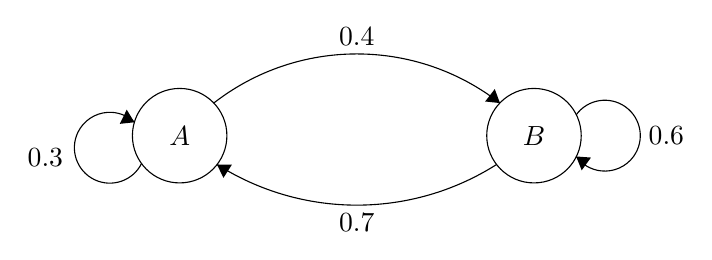
\begin{tikzpicture}[scale=0.2]
	\tikzstyle{every node}+=[inner sep=0pt]
	\draw [black] (19.6,-21) circle (3);
	\draw (19.6,-21) node {$A$};
	\draw [black] (42.1,-21) circle (3);
	\draw (42.1,-21) node {$B$};
	\draw [black] (21.764,-18.93) arc (127.91446:52.08554:14.786);
	\fill [black] (39.94,-18.93) -- (39.61,-18.04) -- (39,-18.83);
	\draw (30.85,-15.31) node [above] {$0.4$};
	\draw [black] (39.727,-22.829) arc (-57.55971:-122.44029:16.549);
	\fill [black] (21.97,-22.83) -- (22.38,-23.68) -- (22.92,-22.84);
	\draw (30.85,-25.91) node [below] {$0.7$};
	\draw [black] (44.78,-19.677) arc (144:-144:2.25);
	\draw (49.35,-21) node [right] {$0.6$};
	\fill [black] (44.78,-22.32) -- (45.13,-23.2) -- (45.72,-22.39);
	\draw [black] (17.184,-22.759) arc (-26.20682:-314.20682:2.25);
	\draw (12.23,-22.39) node [left] {$0.3$};
	\fill [black] (16.73,-20.15) -- (16.24,-19.35) -- (15.8,-20.25);

	\end{tikzpicture}
\end{center}
	
	
\end{przyklad}

Inną równoważną definicją jest trójka $ \langle Q,\pi, p \rangle$, którą definiuje się w sposób następujący:

\begin{definicja}
	Łańcuchem Markowa nazywamy trójkę $ \langle Q,\pi, p \rangle$, gdzie:
	\begin{itemize}
		\item $Q$ jest przestrzenią stanów,
		\item $p: Q \times Q \rightarrow \lbrack 0, 1 \rbrack$ - prawdopodobieństwo osiągnięcia stanu w momencie przejścia,
		\item $\pi: Q \rightarrow \lbrack 0, 1 \rbrack$ - prawdopodobieństwo osiągnięcia stanu inicjalizującego. 
	\end{itemize}
	
	Ponadto muszą zachodzić warunki:
	\begin{itemize}
		\item dla $q_{i} \in Q$, $\sum_{q_{j} \in Q} a(q_{i}, q_{j}) = 1$,
		\item $\sum_{q \in Q} \pi(q) = 1.$
	\end{itemize}	
\end{definicja}

\begin{przyklad}
	Student raz w tygodni bierze udział w zajęciach z rachunku prawdopodobieństwa. Na każde zajęcia przychodzi przygotowany bądź nie. Jeśli w danym tygodniu jest przygotowany, to w następnym jest przygotowany z prawdopodobieństwem 0.7. Jeśli natomiast w danym tygodniu nie jest przygotowany, to w następnym jest przygotowany z prawdopodobieństwem 0.2. Interesujące są pytania na odpowiedzi:
	
	\begin{enumerate}
		\item Jeśli student jest w tym tygodniu nieprzygotowany, to ile tygodni musimy średnio czekać aż będzie przygotowany?
		\item Na dłuższą metę, jak często student jest przygotowany?
	\end{enumerate}
	
	Wyróżniamy tutaj dwa stany: 1 - student jest przygotowany, oraz 2 - student nie jest przygotowany. Na podstawie danych można skonstruować macierz przejścia:\newline
	\[
	M = 
	\begin{bmatrix}
		0.7 & 0.3 \\
		0.2 & 0.8 
	\end{bmatrix}\\
	\]
	Dane: zbiór stanów $S \subseteq \mathcal{R}$, $S = \{0,1\} $. Prawdopodobieństwa zdarzeń przedstawiają się w sposób następujący: \\ \\ 
	$P(X_{t_{2}} = 0 | X_{t_{2}} = 1) = 0.3 = p_{1,0}$ \\
	$P(X_{t_{2}} = 1 | X_{t_{2}} = 1) = 0.7 = p_{1,1}$ \\
	$P(X_{t_{2}} = 1 | X_{t_{2}} = 0) = 0.2 = p_{0,1}$ \\
	$P(X_{t_{2}} = 0 | X_{t_{2}} = 0) = 0.8 = p_{0,0}$ \\
		
	Wiersze macierzy $M$ zgodnie z definicją macierzy przejścia sumują się do 1. 
	Przypuśćmy, że znany jest rozkład zmiennej $\mathnormal{X_{t}}$ czyli prawdopodobieństwo tego, że w chwili $\mathnormal{t}$ znajdujemy się w poszczególnych stanach. Trzeba znaleźć rozkład zmiennej $\mathnormal{X_{t+1}}$ oraz ogólniej rozkład zmiennej $\mathnormal{X_{t+s}}$. Taki rozkład można łatwo znaleźć korzystając z macierzy $\mathnormal{M}$. \\
	Ze wzoru na prawdopodobieństwo całkowite wynika:
	\begin{center}
		$P(X_{t+1} = a) = \sum_{b \in \mathcal{S}} P(X_{t} = b)P(X_{t+1} = a | X_{t} = b) = \sum_{b \in \mathcal{S}} \pi(t)_{b} M_{b,a}$
	\end{center}
	Mówiąc prościej, mamy tutaj do czynienia z mnożeniem macierzy przez wektor, co można zapisać: $\pi(t) \cdot M = \pi(t+1)$
	
\end{przyklad}

\begin{przyklad}
Firmy ubezpieczeniowe wykorzystują łańcuchy Markowa do obliczenia ile rzeczywiście pieniędzy pobierają od swoich klientów. Przykładowym modelem, na którym można to zbadać jest model podsumowujący stan zdrowia człowieka w cyklu miesięcznym.\\

Dane: zbiór stanów $S \subseteq \mathcal{R}$, $S = \{1, 2, 3\} $. gdzie $1$ - oznacza osobę zdrową, $2$ - oznacza osobę chorą, $3$ - oznacza śmierć. Prawdopodobieństwa zdarzeń przedstawiają się w następujący sposób. \\ \\ 
$P(X_{n} = 1 | X_{n} = 2) = 0.3 = p_{2,1}$ \\
$P(X_{n} = 1 | X_{n} = 1) = 0.6 = p_{1,1}$ \\
$P(X_{n} = 2 | X_{n} = 1) = 0.8 = p_{1,2}$ \\
$P(X_{n} = 2 | X_{n} = 2) = 0.1 = p_{2,2}$ \\

Prawdopodobieństwa można zobrazować w postaci automatu z przejściami:

\begin{center}
	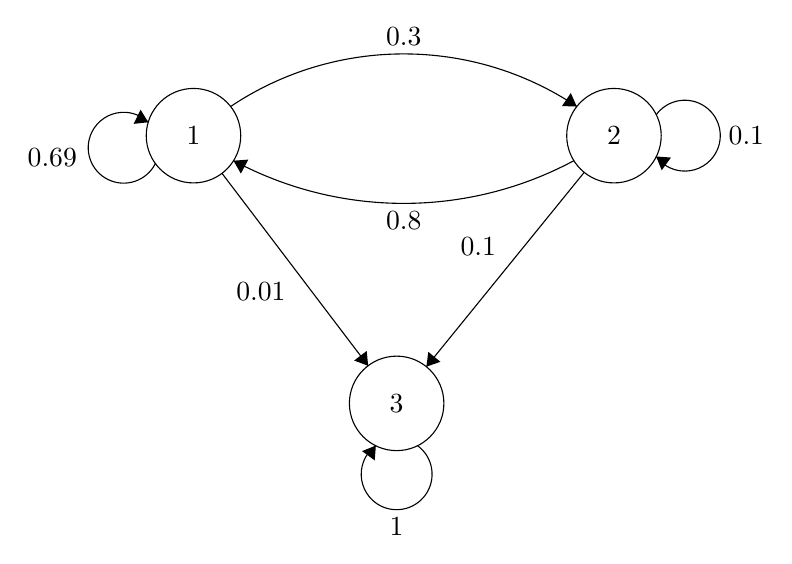
\begin{tikzpicture}[scale=0.2]
	\tikzstyle{every node}+=[inner sep=0pt]
	\draw [black] (19.9,-21.2) circle (3);
	\draw (19.9,-21.2) node {$1$};
	\draw [black] (46.6,-21.2) circle (3);
	\draw (46.6,-21.2) node {$2$};
	\draw [black] (32.8,-38.2) circle (3);
	\draw (32.8,-38.2) node {$3$};
	\draw [black] (22.257,-19.348) arc (123.80513:56.19487:19.759);
	\fill [black] (44.24,-19.35) -- (43.86,-18.49) -- (43.3,-19.32);
	\draw (33.25,-15.51) node [above] {$0.3$};
	\draw [black] (44.057,-22.787) arc (-61.79923:-118.20077:22.868);
	\fill [black] (22.44,-22.79) -- (22.91,-23.61) -- (23.38,-22.72);
	\draw (33.25,-26) node [below] {$0.8$};
	\draw [black] (49.28,-19.877) arc (144:-144:2.25);
	\draw (53.85,-21.2) node [right] {$0.1$};
	\fill [black] (49.28,-22.52) -- (49.63,-23.4) -- (50.22,-22.59);
	\draw [black] (17.484,-22.959) arc (-26.20682:-314.20682:2.25);
	\draw (12.53,-22.59) node [left] {$0.69$};
	\fill [black] (17.03,-20.35) -- (16.54,-19.55) -- (16.1,-20.45);
	\draw [black] (21.71,-23.59) -- (30.99,-35.81);
	\fill [black] (30.99,-35.81) -- (30.9,-34.87) -- (30.1,-35.48);
	\draw (25.78,-31.1) node [left] {$0.01$};
	\draw [black] (44.71,-23.53) -- (34.69,-35.87);
	\fill [black] (34.69,-35.87) -- (35.58,-35.56) -- (34.81,-34.93);
	\draw (39.14,-28.27) node [left] {$0.1$};
	\draw [black] (34.123,-40.88) arc (54:-234:2.25);
	\draw (32.8,-45.45) node [below] {$1$};
	\fill [black] (31.48,-40.88) -- (30.6,-41.23) -- (31.41,-41.82);
	\end{tikzpicture}
\end{center}

Brakujące prawdopodobieństwa zostały wyliczone biorąc pod uwagę własność macierzy przejścia, w której wiersze sumują się do 1. \\
$p_{1,1} = 1 - p_{1,2} - p_{1,3}$ oraz $p_{2,2} = 1 - p_{2,1} - p_{2,3}$. Na podstawie powyższego łańcuchy Markowa można próbować odpowiedzieć na pytania:

\begin{itemize}
	\item Jaka jest długość życia obecnie zdrowej osoby?
	\item Jaka jest długość życia obecnie chorej osoby?
\end{itemize}

\end{przyklad}


\begin{przyklad}
 
	Niech dane będą dwie zmienne losowe $X_{0}, X_{1}$, gdzie $X_{0}$ oznaczać będzie pogodę słoneczną, a $X_{1}$ oznaczać będzie pogodę pochmurną. Dla ułatwienia wprowadźmy oznaczenia: $X_{0} - S$, $X_{1} - C$. Następnie przypiszmy prawdopodobieństwo wystąpienia pogody słonecznej równe $\frac{1}{2}$ oraz prawdopodobieństwo wystąpienia pogody pochmurnej równe $\frac{1}{2}$. Następnym krokiem będzie wygenerowanie losowej pogody na 356, gdzie taki rozkład można zaprezentować za pomocą symboli np. $S,S,C,C,S,S,S,C,S,C,S,C, ..., n$. Mając rozkład w postaci symboli można go zobrazować w postaci wykresu.
 
	
	\begin{figure}[H]
		\centering
		\includegraphics[width=0.7\linewidth]{wykres_pogoda}
		\caption[ ]{Wykres prawdopodobieństwa}
		\label{fig:wykrespogoda}
	\end{figure}
	Powyższa ilustracja obrazuje działanie modelu, pogoda każdego dnia jest niezależna od poprzednich dni, pobierana jest również z tego samego rozkładu. W następnym kroku wykorzystamy łańcuch Markowa i macierz przejścia aby uzależnić dany stan od poprzedniego. Łańcuch Markowa rozpocznie się w określonym stanie, a następnie pozostanie w tym samym stanie lub przejdzie do innego stanu na podstawie macierzy prawdopodobieństw:
	
	\[
	P = 
	\begin{bmatrix}
	0.7 & 0.3 \\
	0.2 & 0.8 
	\end{bmatrix}\\
	\]
	
	Z macierzy możemy odczytać, że prawdopodobieństwo zajścia dnia słonecznego pod warunkiem, że poprzedniego dnia był słoneczny dzień wynosi 0.7

\begin{figure}[H]
\begin{center}
	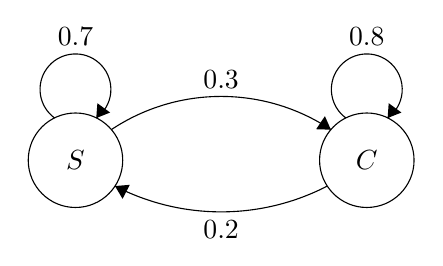
\begin{tikzpicture}[scale=0.2]
	\tikzstyle{every node}+=[inner sep=0pt]
	\draw [black] (23,-25.8) circle (3);
	\draw (23,-25.8) node {$S$};
	\draw [black] (41.5,-25.8) circle (3);
	\draw (41.5,-25.8) node {$C$};
	\draw [black] (21.677,-23.12) arc (234:-54:2.25);
	\draw (23,-18.55) node [above] {$0.7$};
	\fill [black] (24.32,-23.12) -- (25.2,-22.77) -- (24.39,-22.18);
	\draw [black] (40.177,-23.12) arc (234:-54:2.25);
	\draw (41.5,-18.55) node [above] {$0.8$};
	\fill [black] (42.82,-23.12) -- (43.7,-22.77) -- (42.89,-22.18);
	\draw [black] (25.276,-23.857) arc (123.65827:56.34173:12.583);
	\fill [black] (39.22,-23.86) -- (38.84,-23) -- (38.28,-23.83);
	\draw (32.25,-21.25) node [above] {$0.3$};
	\draw [black] (38.994,-27.439) arc (-62.66466:-117.33534:14.686);
	\fill [black] (25.51,-27.44) -- (25.99,-28.25) -- (26.45,-27.36);
	\draw (32.25,-29.58) node [below] {$0.2$};
	\end{tikzpicture}
	\caption{Graf prawdopodobieństw równoważny z macierzą przejść}
\end{center}
\end{figure}

Należy stworzyć zmienną losową dla każdego rzędu macierzy przejścia, zmienna losowa odpowiada prawdopodobieństwom przejść od stanu do stanu. 

\begin{figure}[H]
	\centering
	\includegraphics[width=0.7\linewidth]{pogoda_markov}
	\caption{Wykres prawdopodobieństwa po zastosowaniu łańcucha Markowa}
	\label{fig:pogodamarkov}
\end{figure}

Jak widać na ilustracji powyżej, po zastosowaniu łańcucha Markowa z zadaną macierzą przejścia wykres wygląda trochę inaczej. Za pomocą macierzy jesteśmy w stanie kontrolować długości danego stanu. Poniżej znajduje się pełen listing kodu programu, który realizuje powyższe rozważania.


\lstinputlisting[language=Python]{markov_chain_var_ex.py}


\end{przyklad}


\subsection{Pojęcia i własności łańcuchów}
	
	W teorii prawdopodobieństwa oraz statystyce rozważa się inne modele matematyczne, które bazują na probabilistyce i są trochę bardziej rozbudowane niż klasyczny łańcuch Markowa. Należy tutaj wymienić takie modele jak: łańcuchy Markowa wyższego rzędu, ukryte modele Markowa, łańcuchy Markowa mieszanego rzędu, łańcuchy Markowa wyższego rzędu, probabilistyczne skończone automaty. Poniżej zostaną przedstawione niektóre z nich.
	

	Rozpoczniemy od opisu ukrytych modeli Markowa. Ukryte modele Markowa (HMM, ang. hidden Markov models) są rozszerzeniem standardowej definicji łańcucha Markowa. Używane są głównie do modelowania związku między ukrytymi, a obserwowanymi sekwencjami. Ukrytym modelem Markowa jest łańcuch Markowa z dyskretnym rozkładem prawdopodobieństwa w każdym stanie. Dyskretne rozkłady prawdopodobieństwa definiują prawdopodobieństwa emisji określonego symbolu alfabetu w danym stanie. 

\begin{definicja}
	Ukrytym modelem Markowa nazywamy piątkę $ \langle \sum, Q, a, b, \pi  \rangle$ gdzie:
	\begin{itemize}
		\item $\sum$ jest skończonym alfabetem widocznych symboli,
		\item $Q$ jest skończonym zbiorem ukrytych stanów,
		\item $a: Q \times Q \rightarrow \lbrack 0, 1 \rbrack$ - prawdopodobieństwo osiągnięcia stanu pomiędzy stanami ukrytymi,
		\item $b: Q \times \sum \rightarrow \lbrack 0, 1 \rbrack$ - prawdopodobieństwo emisji określonego symbolu alfabetu w danym ukrytym stanie,
		\item $\pi: Q \rightarrow \lbrack 0, 1 \rbrack$ - początkowe prawdopodobieństwo ukrytych stanów.
	\end{itemize}
	Ponadto muszą zachodzić warunki:
	\begin{itemize}
		\item dla $q_{i} \in Q$, $\sum_{q_{j} \in Q} a(q_{i}, q_{j}) = 1$,
		\item $\sum_{q \in Q} \pi(q) = 1.$
	\end{itemize}	
	
	Oznaczmy sekwencję obserwacji i stanu ukrytego przez $X = X_{1}, ..., X_{n}$ i $s = s_{1}, ..., s_{n}$, gdzie $X_{i} \in \sum$ oraz $s_{i} \in Q$. W tym przypadku używamy następującej notacji:
	\begin{center}
		$\pi(q_{i}) = P(s_{1} = q_{i})$ \\
		$a(q_{i},q_{j}) = P(s_{t} = q_{j} | s_{t-1} = q_{i})$ \\
		$b(q_{j},X_{t}) = P(X_{t} | s_{t} = q_{j})$
	\end{center}  
	$P(x)$ jest prawdopodobieństwem zdarzenia, natomiast $P(x | y)$ jest prawdopodobieństwem zdarzenia $x$ pod warunkiem $y$.
\end{definicja}

\begin{przyklad}
	Klasycznym przykładem ukrytego łańcucha Markowa jest nieuczciwe kasyno do gry, które ma dwa rodzaje kości: uczciwą kostkę do gry (z prawdopodobieństwem $\frac{1}{6}$ wyrzuca się każda z sześciu możliwych wartości) oraz nieuczciwą kostkę (dla której prawdopodobieństwo wyrzucenia szóstki wynosi $\frac{1}{2}$, a dla pozostałych liczb $\frac{1}{10}$). Mamy do dyspozycji dwa stany: F (uczciwa kostka) i L (nieuczciwa kostka). Układ może zmieniać swój stan z pewnym prawdopodobieństwem, ale my stanu nie możemy zaobserwować (np. krupier zmienia kostki pod stołem). Jedynie widzimy ciąg liczb będących wynikiem rzutów kostką. To, którą kostką rzucamy zależy tylko i wyłącznie od stanu ukrytego łańcucha Markowa. Macierz przejścia zdefiniujemy następująco:
	\[
		P = 
		\begin{bmatrix}
		0.9 & 0.1 \\
		0.45 & 0.55 
		\end{bmatrix}\\
	\]
	gdzie $p_{F,F}=0.90$, $p_{L,L}=0.55$, $p_{F,L}=0.10$, $p_{L,F}=0.45$. Średni czas nieprzerwanego rzucania kostką uczciwą jest równy $\frac{1}{1-0.9} = 10$ okresów, a kostką fałszywą $ \frac{1}{0.55} = 2$. Chodź nie wiemy, którą kostką rzucamy to mamy o tym jednak jakąś informacje. Obserwujemy bowiem ciąg liczb będących wynikiem rzutów kostką. Macierz emisji dla tego przykładu wygląda następująco:
	
	\[
	\prod = 
	\begin{bmatrix}
	\frac{1}{6} & \frac{1}{6} & \frac{1}{6} & \frac{1}{6} & \frac{1}{6} & \frac{1}{6} \\
	\frac{1}{10} & \frac{1}{10} & \frac{1}{10} & \frac{1}{10} & \frac{1}{10} & \frac{1}{2} &
	\end{bmatrix}\\
	\]
		 
\end{przyklad}

\begin{przyklad}
	Ukryty łańcuch Markowa można również wykorzystać w muzyce do generowania akordów na podstawie progresji II V I. Progresja II V I jako następstwo akordów, jest wykorzystywana w szerokim zakresie gatunków muzycznych oraz jest podstawą harmonii jazzowej. W przykładzie będziemy rozważać progresje II V I dla akordów tonacji C-dur. Poszczególne akordy będą stanami w łańcuchu Markowa. Stany ukryte będą odpowiedzialne za typ akordu (minor7, major7, dominant7).
	
 \begin{figure}[H]
 	\centering
 	\includegraphics[width=0.7\linewidth]{akordy}
 	\caption{Podstawowe rodzaje akordów dla gamy C-dur}
 	\label{fig:akordy}
 \end{figure}

	W pierwszym kroku należy zdefiniować macierz przejścia dla stanów łańcucha Markowa. W przykładzie będą wykorzystane trzy stany, które będą odpowiadały nutą D, G, C - progresja II V I.
	
	\[
	P = 
	\begin{bmatrix}
	0.4 & 0.4 & 0.2 \\
	0.1 & 0.1 & 0.8 \\
	0.0 & 0.3 & 0.7 
	\end{bmatrix}\\
	\]
 
	Następnie musi zostać stworzona macierz emisji dla stanów ukrytych. Warstwa ukryta będzie odpowiedzialna za rodzaj akordu. Do dyspozycji będą trzy rodzaje akordów: minor7, major7, dominant7.
	
	\[
	M = 
	\begin{bmatrix}
	0.4 & 0.0 & 0.4 \\
	0.3 & 0.3 & 0.3 \\
	0.2 & 0.8 & 0.0 
	\end{bmatrix}\\
	\]
	 
	Dla danego stanu z macierzy $P$ będzie wybierany dany stan z macierzy $M$ z uwzględnieniem reguł łańcucha Markowa. Praktycznie zostanie to zrealizowane z użyciem języka Python. Pakiet o nazwie $hmmlearn$ zwolni nas z implementowania logiki Ukrytego Modelu Markowa, a za pomocą pakietu $music21$ będzie można wygenerować akordy na pięciolinii. 
	
	\begin{lstlisting}[caption={Ukryty Model Markowa z użyciem Pythona},captionpos=b]
 import numpy as np
 from hmmlearn import hmm
 from music21 import *
 
 environment.set("musescoreDirectPNGPath",     "/usr/bin/musescore")
 environment.set("musicxmlPath",     "/usr/bin/musescore")
 environment.set("midiPath",     "/usr/bin/lilypond")
 
 conv = converter.subConverters.ConverterLilypond()
 
 
 transmat = np.array([[0.4, 0.4, 0.2],
 [0.1, 0.1, 0.8],
 [0.0, 0.3, 0.7]])
 
 start_prob = np.array([1.0, 0.0, 0.0])
 
 emission_probs = np.array([[0.4, 0.0, 0.4],
 [0.3, 0.3, 0.3],
 [0.2, 0.8, 0.0]])
 
 chord_model = hmm.MultinomialHMM(n_components=2)
 
 chord_model.startprob_ = start_prob
 
 chord_model.transmat_ = transmat
 chord_model.emissionprob_ = emission_probs
 X, Z = chord_model.sample(10)
 
 state2name = {}
 state2name[0] = 'D'
 state2name[1] = 'G'
 state2name[2] = 'C'
 chords = [state2name[state] for state in Z]
 
 obj2name = {}
 obj2name[0] = 'min7'
 obj2name[1] = 'maj7'
 obj2name[2] = '7'
 
 observations = [obj2name[item] for sublist in X for item in sublist]
 chords = [''.join(chord) for chord in zip(chords, observations)]
 
 
 # create some chords for II, V, I
 d7 = chord.Chord(['D4', 'F4', 'A4', 'C5'])
 dmin7 = chord.Chord(['D4', 'F-4', 'A4', 'C5'])
 dmaj7 = chord.Chord(['D4', 'F#4', 'A4', 'C#5'])
 
 c7 = d7.transpose(-2)
 cmin7 = dmin7.transpose(-2)
 cmaj7 = dmaj7.transpose(-2)
 
 g7 = d7.transpose(5)
 gmin7 = dmin7.transpose(5)
 gmaj7 = dmaj7.transpose(5)
 print(g7.pitches)
 
 stream1 = stream.Stream()
 stream1.repeatAppend(dmin7, 1)
 stream1.repeatAppend(g7, 1)
 stream1.repeatAppend(cmaj7, 1)
 stream1.repeatAppend(cmaj7, 1)
 print(stream1)
 
 name2chord = {}
 name2chord['C7'] = c7
 name2chord['Cmin7'] = cmin7
 name2chord['Cmaj7'] = cmaj7
 
 name2chord['D7'] = d7
 name2chord['Dmin7'] = dmin7
 name2chord['Dmaj7'] = dmaj7
 
 name2chord['G7'] = g7
 name2chord['Gmin7'] = gmin7
 name2chord['Gmaj7'] = gmaj7
 hmm_chords = stream.Stream()
 
 for c in chords:
 	hmm_chords.repeatAppend(name2chord[c], 1)
 
 hmm_chords.show()
	\end{lstlisting}
	W przykładzie użyto 10 iteracji. Wynikiem działania programu jest sekwencja akordów przedstawiona poniżej:
	
	\begin{figure}[H]
		\centering
		\includegraphics[width=0.7\linewidth]{hmm_music_notes}
		\caption{Wygenerowane akordy z użyciem ukrytego modelu Markowa}
		\label{fig:hmmmusicnotes}
	\end{figure}
	
	
	
\end{przyklad}

Powyższy kod został wzbogacony o interfejs użytkownika, w którym można definiować wartości macierzy prawdopodobieństw i emisji.

\begin{figure}[H]
	\centering
	\includegraphics[width=0.7\linewidth]{hidden_markov_python}
	\caption{Interfejs aplikacji, która wykorzystuje ukryte modele Markowa do generowania akordów}
	\label{fig:hiddenmarkovpython}
\end{figure}


\begin{figure}[H]
	\centering
	\includegraphics[width=0.7\linewidth]{hidden_markov_python_result}
	\caption{Wygenerowane akordy na podstawie zadanych macierzy}
	\label{fig:hiddenmarkovpythonresult}
\end{figure}

W programie wykorzystano bibliotekę music21, która posłużyła do zapisu nutowego oraz zapisu nut do pliku. Algorytm ukrytego modelu Markowa pochodzi z biblioteki hmmlearn.

Możemy powiedzieć, że standardowe Łańcuchy Markowa maja pamięć długości 1 ponieważ n-ty stan zależy tylko i wyłącznie od stanu poprzedniego. Przeciwieństwo stanowią Łańcuchy Markowa wyższego rzędu (ang. Higher Order Markov Chains), które mają pamięć większą niż jeden. 

\begin{definicja}
	Łańcuch Markowa N-tego rzędu definiujemy w następujący sposób:
	\begin{center}
		
		$P(q_{t} | q_{t-1}, q_{t-2}, ..., q_{1}) = P(q_{t} | q_{t-1}, ..., q_{t-min(t-1, N)})$
		
	\end{center}
	Jeżeli $t \leq N$ to $q_{t}$ jest stanem startowym oraz nadmierne stany $q_{t}$ gdzie $t \le 0$ są reprezentowane przez puste słowo $\lambda$. W przypadku Łańcucha Markowa N-tego rzędu będziemy używać zapisu $a(q_{t-N}, ..., q_{t-1}, q_{t})$ zamiast $a(q_{t-1}, q_{t})$ aby wskazać prawdopodobieństwa przejścia. 
\end{definicja}


\subsection{Zastosowania Łańcuchów Markowa}

Łańcuchy Markowa mają bardzo szerokie zastosowanie, możemy tutaj wskazać takie dyscypliny nauki jak: fizyka, genetyka, meteorologia, gospodarka. Przydatność łańcuchów Markowa uwidacznia się w przypadku, gdy nie można przyjąć założenia o niezależności zdarzeń i zmiennych losowych. Do zalet prognozowania na podstawie łańcuchów Markowa można zaliczyć:
\begin{itemize}
	\item możliwość predykcji w przypadku, gdy nie są znane przyczyny występowania badanego zjawiska lub gdy jest ich zbyt wiele,
	\item możliwość konstruowania prognoz dla zjawisk mierzalnych i niemierzalnych,
	\item możliwość budowy prognoz krótko, średnio, oraz długoterminowych,
	\item możliwość prognozowania strukturalnych zjawisk ekonomicznych o wzajemnie zależnych w czasie elementach składowych
\end{itemize}
	
	Jednym z ciekawszych zastosowań łańcuchów Markowa jest użycie ich w popularnym algorytmie wyszukiwarki \textbf{Google - PageRank}. Algorytm można interpretować jako znajdowanie ustalonego stanu z łańcucha Markowa. W tym przypadku łańcuch Markowa jest modelem procesu poruszania się użytkownika po zbiorze wszystkich stron www. Każda strona jest stanem, a powiązania między stronami są prawdopodobieństwami. Niezależnie od tego na jakiej stronie się znajdujemy szansa na znalezienie się na innej stronie X określone jest stałym prawdopodobieństwem. Formalnie: jeżeli $N$ jest liczbą wszystkich znanych stron internetowych oraz strona $i$ posiada $k_{i}$ linków prowadzących do niej wówczas można ustalić prawdopodobieństwo przejścia $\frac{\alpha}{k_{i}} + \frac{1-\alpha}{N}$ dla wszystkich stron, które są połączone z daną stronę i $\frac{1-\alpha}{N}$, które nie są połączone, gdzie $\alpha$ jest stałą równą 0.85\pagenote{\texttt{http://citeseerx.ist.psu.edu/viewdoc/summary?doi=10.1.1.31.1768}}. Łańcuch Markowa pozwala również na analizę zachowania użytkownika podczas nawigacji na stronie internetowej. Na podstawie takiej analizy można np. spersonalizować nawigację pod danego użytkownika. 
 
	Większość popularnych klawiatur na systemy Android umożliwia szybsze pisanie wiadomości poprzez \textbf{podpowiadanie następnych słów} na podstawie poprzednich. Słowa, które piszemy są analizowane i włączane do prawdopodobieństwa w łańcuchu Markowa. Czasami aplikacje proszą o możliwość dostępu np. do emaili aby na ich podstawie zbudować bazę prawdopodobieństw. Mając bazę prawdopodobieństw, czyli w tym wypadku łańcuch Markowa, aplikacje wykorzystują model probabilistyczny n-gram, który jest wykorzystywany do pobierania kolejnego elementu z sekwencji łańcucha Markowa. 
  	
	Ukryte modele Markowa mają swoje zastosowanie w systemach do \textbf{automatycznego rozpoznawania mowy}. Za ich pomocą tworzy się modele akustyczne, które odpowiadają danemu wyrazowi. Najbardziej popularnym algorytmem, który jest wykorzystywany przy rozpoznawaniu mowy jest algorytm Bauma-Welcha. Systemy do rozpoznawania mowy możemy podzielić na dwa rodzaje: systemy rozpoznawania mowy ciągłej oraz systemy rozpoznawania wystąpień izolowanych słów. Główną ideą ukrytych modeli Markowa jest traktowanie sygnału mowy jako sekwencji wektorów obserwacji, które z jednej strony stanowią ciąg uczący w procesie uczenia, podczas gdy tworzony jest model akustyczny mówcy, a z drugiej strony są wyjściem modeli w tworzonym procesie weryfikacji \pagenote{\texttt{http://www.kms.polsl.pl/mi/pelne\_9/31.pdf}}. 

	Łańcuchy Markowa stosuje się również do \textbf{generowania sekwencji liczb losowych} w celu dokładnego odzwierciedlenia bardzo skomplikowanych rozkładów prawdopodobieństw. Metoda, która wykorzystuje łańcuch Markowa do generowania sekwencji liczb nosi nazwę Łańcuch Markowa Monte Carlo. W ostatnich latach wymieniona wcześniej metoda zrewolucjonizowała metody wnioskowania bayesowskiego, pozwalając na symulacje szerokiego zakresu rozkładów w odcinku bocznym i ich parametrów. 

	Łańcuchy Markowa mają również swoje zastosowanie w \textbf{ modelowaniu biologicznym} szczególnie w procesach populacyjnych. Stan łańcucha Markowa w procesie populacyjnym jest analogiczny do liczby osobników w danej populacji (0, 1, 2, 3, ..., n) zmiany stanu są analogiczne do dodawania lub usuwania osób z danej populacji. Jednym z takich przykładów jest macierz Lesli, która opisuje dynamikę populacji wielu gatunków. Innym przykładem jest modelowanie kształtu komórek w dzielących się segmentach komórek nabłonka. Łańcuchy Markowa są również wykorzystywane w symulacjach funkcji mózgu takich jak symulacja kory nowe, która jest odpowiedzialna za odbieranie i przetwarzanie wrażeń zmysłowych, planowanie i wykonywanie ruchów dowolnych oraz procesy poznawcze (pamięć, myślenie, funkcje językowe). 

	Łańcuchy Markowa są używane w celu \textbf{przetwarzania informacji}. Teoria informacji, która wprowadza pojęcie entropii wykorzystuje łańcuchy Markowa w celu efektywnej kompresji danych za pomocą technik kodowania entropijnego - kodowanie arytmetyczne. Przykładem algorytmy do kompresji danych jest bezstratny algorytm LZMA\pagenote{\texttt{https://en.wikipedia.org/wiki/Lempel-Ziv-Markov\_chain\_algorithm}}, który łączy łańcuchy Markowa z kompresją Lempel-Ziv\pagenote{\texttt{https://en.wikipedia.org/wiki/LZ77\_and\_LZ78}} aby osiągnąć bardzo wysokie współczynniki kompresji. Jako prekursora teorii informacji uważa się Clauda Shannona i jego dzieło z 1948 roku "A Mathematical Theory of Communication". Ukryte Modele Markowa, które mają swoją podstawę w Łańcuchach Markowa są ważnym narzędziem w sieciach telefonicznych. Dużą rolę odgrywa tutaj algorytm Viterbiego, który jest wykorzystywany do korekcji błędów.

	Łańcuchy Markowa wykorzystywane są również w \textbf{finansach i ekonomii}. Za ich pomocą modeluje się różne zjawiska, między innymi ceny aktywów i krachy rynkowe. Dynamiczna makroekonomia w dużym stopniu wykorzystuje łańcuchy Markowa. Przykładam jest wykorzystanie łańcuchów Markowa do egzogenicznego modelowania cen kapitału własnego w ogólnym ustawieniu równowagi. Innym przykładem jest sporządzenie przez agencje ratingowe rocznych tabeli prawdopodobieństw przejścia dla obligacji o różnych ratingach kredytowych. 
	
	Łańcuchy Markowa są szeroko stosowane w \textbf{termodynamice i mechanice statystycznej}. Prawdopodobieństwa są używane do reprezentowania nieznanych lub niezmodyfikowanych szczegółów systemu, jeśli można założyć, że dynamika jest niezmienna w czasie i nie należy brać pod uwagę odpowiedniej historii, która nie została jeszcze uwzględniona w opisie stanu. Łańcuchy Markowa są również wykorzystywane praktycznie do symulacji sieci chromodynamiki kwantowej, która to ma za zadanie opisanie oddziaływań silnych (kwantowa teoria pola).
	


\subsection{Łańcuchy Markowa w muzyce}

Pierwszą osobą, która użyła łańcuchów Markowa do kompozycji muzyki był kompozytor rumuńsko - francuskiego pochodzenia Iannis Xenakis. Muzyk w 1958 roku użył łańcuchów Markowa w kompozycji Analogique$\pagenote{\texttt{https://www.youtube.com/watch?v=mXIJO-af\_u8}}$. Swoją pracę opisał w książce "Formalized Music: Thought and Mathematics in Composition $\pagenote{Iannis Xenakis. \textit{Formalized Music Thought and mathematics in composition}, Pendragon Press, 1992}



Utwór muzyczny jest reprezentowany przez sekwencję zdarzeń, które są obiektami muzycznymi. Każdy obiekt muzyczny czyli nuta posiada dwie wartości: częstotliwość dźwięku, która reprezentowana jest przez literkę nuty oraz długość trwania. Linearna budowa utworu muzycznego pozwala na wyodrębnienie struktury fraz i polifonii. Biorąc pod uwagę statystyczny model w kontekście utworu muzycznego, możemy przypisać prawdopodobieństwo wystąpienia danej nuty w sekwencji. Dlatego też łańcuchy Markowa mają swoje zastosowanie w dziedzinie jaką jest algorytmiczne komponowanie muzyki. Można tutaj wymienić przykłady programowania odwołując się do programów CSound, Max, SuperCollider.

Istnieje wiele formatów, które umożliwiają zapis utworu muzycznego w formacie cyfrowym, który umożliwia jego odtworzenie na komputerze. Możemy wymieć tu powszechnie używane formaty plików takie jak mp3, flac czy wav. Jednak za pomocą tych formatów nie jesteśmy w prosty sposób wyodrębnić poszczególnych nut utworu muzycznego. W tym celu można się posłużyć innym sposobem zapisu muzyki. Formaty MIDI oraz MusicXML pozwalają zapisać utwór muzyczny nuta po nucie, dzięki temu też istnieje możliwość odczytania pełnego zapisu nutowego danego utworu zapisanego w jednym z tych formatów. 

Standard MIDI (Musical Instrument Interface) został opracowany z myślą o komunikacji elektronicznych instrumentów muzycznych. Plik MIDI może się składać z wielu ścieżek, z których każda odpowiada brzmieniu określonego instrumentu. Należy mieć na uwadze, że pliki MIDI nie są plikami muzycznymi tak jak np. popularny format MP3 czy FLAC. W plikach MIDI znajdują się tylko instrukcje mówiące o tym jak dana nuta ma być zagrana. Następnie z wykorzystaniem samplera można odczytać taki plik co spowoduje w konsekwencji odegranie pewnego kawałka muzyki, który to jest reprezentowany przez dane tekstowe. Format MIDI może przechowywać tylko ograniczoną ilość informacji, nie można w nim zawrzeć chociażby słów utworu. Informacje o dźwięku zapisywane są w postaci tak zwanych zdarzeń. Przykładowe dwa zdarzenia MIDI zostały zaprezentowane w tabeli poniżej.
\begin{table}[H]
	$$\begin{tabular}{|c|c|c|c|c|}
	\hline 
	\textbf{typ zdarzenia} & \textbf{time} & \textbf{channel} & \textbf{note} & \textbf{velocity} \\ 
	\hline 
	note\_on & 0 & 0 & 67 & 127 \\ 
	\hline 
	note\_off & 400 & 0 & 67 & 0 \\ 
	\hline 
	\end{tabular} $$
	\caption{Dwa zdarzenia MIDI}
	
\end{table}


Natomiast odczyt zdarzenia wygląda następująco:

\begin{lstlisting}[caption={Odczyt pliku MIDI},captionpos=b]
Track 0: 
note_on channel=0 note=60 velocity=127 time=192
note_off channel=0 note=60 velocity=64 time=192
<meta message end_of_track time=0>
\end{lstlisting}

Aby skonstruować prosty plik MIDI, którego zadaniem będzie zapisanie trzech nut: C, E, G posłużymy się językiem Python i pakietem mido. 

\begin{lstlisting}[caption={Skrypt w Pythonie realizujący zapis określonych nut do pliku MIDI},captionpos=b]
	import mido
	filename="outfile.mid"
	def note_to_message(note):
		return [
		mido.Message('note_on', note=note, velocity=127, time=192),
		mido.Message('note_off', note=note, velocity=64, time=192)
		]
	def read_midi(filename):
		mid = mido.MidiFile(filename)
		for i, track in enumerate(mid.tracks):
			print 'Track {}: {}'.format(i, track.name)
			for message in track:
				print message
	with mido.midifiles.MidiFile() as midi:
		track = mido.MidiTrack()
		notes = [60, 64, 67]
		for i in notes:
			track.extend(note_to_message(i))
			midi.tracks.append(track)
		midi.save(filename)
\end{lstlisting}

Następnie strukturę stworzonego pliku można odczytać za pomocą funkcji read\_midi. Jej wynik jest zaprezentowany poniżej:

\begin{lstlisting}
	Track 0: 
	note_on channel=0 note=60 velocity=127 time=192
	note_off channel=0 note=60 velocity=64 time=192
	note_on channel=0 note=64 velocity=127 time=192
	note_off channel=0 note=64 velocity=64 time=192
	note_on channel=0 note=67 velocity=127 time=192
	note_off channel=0 note=67 velocity=64 time=192
	<meta message end_of_track time=0>
\end{lstlisting}

Jedno zdarzenie jest reprezentowane przez cztery zmienne: time, channel, note, velocity. Zmienna time określa czas danego zdarzenia. Channel wskazuje jeden z 16 kanałów (0-15) do którego dane zdarzenie ma należeć. Poszczególne nuty nie są reprezentowane w postaci symboli A, H, G tylko w postaci liczb z zakresu od 0 do 127. Tabela poniżej przedstawia reprezentacje wszystkich możliwych nut w postaci liczbowej.
\begin{figure}[H]
	\centering
	\includegraphics[width=0.7\linewidth]{nutymidi.jpg}
	\caption{Reprezentacja nut w formacie MIDI}
	\label{fig:fwxnbxgh4afzwe7}
\end{figure}

Nawiązując do powyżej tabeli, która reprezentuje dwa zdarzenia MIDI numery 67 oznaczają nutę G4. Kolejna zmienna o nazwie velocity przyjmuje wartości z zakresu (0-127). Jej zadaniem jest określenie siły danego dźwięku, inaczej mówiąc im mniejsza wartość zmiennej velocity tym dźwięk jest bardziej cichy. Pliki MIDI zawierają wszystkie istotne dane muzyczne, możliwe jest więc określenie prawdopodobieństwa przejścia z jednej nuty na drugą poprzez odpowiednią analizę pliku.

Innym dostępym formatem służącym do zapisu informacji o utworze muzycznym jest standard MusicXML$\pagenote{\texttt{http://www.musicxml.com/}}$. Jest to znacznikowy format prezentacji graficznej notacji muzycznej, który oparty jest na wzorcach dokumentowych DTD$\pagenote{\texttt{https://en.wikipedia.org/wiki/Document\_type\_definition}}$. Aby zrozumieć notację zapisu MusicXML wystarczy podstawowa znajomość języka XML, który jest dość powszechnie wykorzystywany. Format MusicXML jest wspierany przez ponad 230 programów służących do zapisu notacji muzycznej takich jak Finale\pagenote{\texttt{https://www.finalemusic.com/}}, Sibelius\pagenote{\texttt{http://www.avid.com/sibelius}} czy MusicScore\pagenote{\texttt{https://musescore.org/pl}}. Poniżej zostanie przedstawiona przykładowa struktura pliku MusicXML.

\begin{lstlisting}
<?xml version="1.0" encoding="UTF-8"?>
<!DOCTYPE score-partwise PUBLIC "-//Recordare//DTD MusicXML 3.1 Partwise//EN"
 "http://www.musicxml.org/dtds/partwise.dtd">
<score-partwise>
	<identification>
		<rights></rights>
		<encoding>
		<software></software>
		<encoding-date></encoding-date>
		</encoding>
	</identification>
	<part-list>
		<score-part id='P1'>
			<part-name>Track 1</part-name>
		</score-part>
	</part-list>
	<part id="P1">
		<measure number='1'>
			<atrributes>atrybut miary</atrributes>
			<note>
				<pitch>
					<step>C</step>
					<octave>4</octave>
				</pitch>
				<duration>96</duration>
				<type>whole</type>
			</note>
		</measure>
	</part>
</score-partwise>
\end{lstlisting}

Pierwsze trzy linijki definiują standard dokumentu XML. Plik partwise.dtd definiuje reprezentacje nut, plik timewise.dtd definiuje długości trwania nut. Następnie występuje główny tag o nazwie \xml{score-partwise}, którego dzieckiem jest tag \xml{identyfication}, którego zadaniem jest przechowywanie meta informacji o pliku. Tag \xml{score-part} reprezentuje ścieżkę utworu. Przykład powyżej posiada jedną ścieżkę, która jest opisana w tagu \xml{measure}. Poszczególna ścieżka posiada takie atrybuty jak tempo, rozmiar, tonację, metrum, klucz.


Bardzo ciekawym zastosowaniem łańcucha Markowa jest wykorzystanie go do generowania muzyki.
Weźmy dla przykładu dwie melodie (c,d,e,c,d,c,d,e,c,d) oraz (d,e,d,e,c,d,c,d,e,d). Podane melodie tworzą przestrzeń stanów $Q=\{c,d,e\}$. Macierz prawdopodobieństw jest obliczana według wzoru:

$$ a(q_{i},q_{j}) = \frac{\#(q_{i} \rightarrow q_{j})}{ \sum_{q_{k} \in Q} \#(q_{i} \rightarrow q_{k})} $$

gdzie $\#(q_{i} \rightarrow q_{j})$ jest ilością możliwych przejść ze stanu $q_{i}$ do stanu $q_{j}$. Macierz prawdopodobieństw wygląda następująco:
\[
a =
\begin{bmatrix}
a(c,c) & a(c,d) & a(c,e) \\
a(d,c) & a(d,d) & a(d,e) \\
a(e,c) & a(e,d) & a(e,e)
\end{bmatrix}
=
\begin{bmatrix}

0 & 1 & 0 \\
\frac{2}{7} & 0 & \frac{5}{7} \\
\frac{4}{5} & \frac{1}{5} & 0 

\end{bmatrix}
\] 

oraz:
$$ \pi = \Big( \pi(c), \pi(d), \pi(e) \Big) = \Big( \frac{1}{2}, \frac{1}{2}, 0 \Big) $$
Graf prawdopodobieństw dla powyższej macierzy przedstawia się w sposób następujący:
\begin{figure}[H]
\begin{center}
	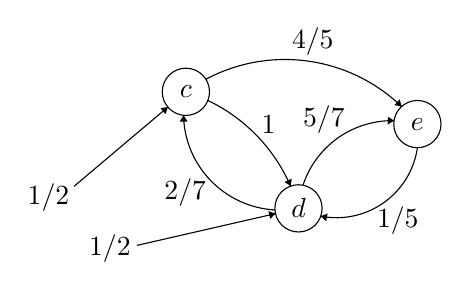
\begin{tikzpicture}[scale=0.1]
	\tikzstyle{every node}+=[inner sep=0pt]
	\draw [black] (29.7,-27.8) circle (3);
	\draw (29.7,-27.8) node {$c$};
	\draw [black] (59.1,-31.9) circle (3);
	\draw (59.1,-31.9) node {$e$};
	\draw [black] (44,-42.6) circle (3);
	\draw (44,-42.6) node {$d$};
	\draw [black] (32.239,-26.207) arc (118.06789:46.05406:21.343);
	\fill [black] (57.09,-29.67) -- (56.86,-28.76) -- (56.17,-29.48);
	\draw (45.82,-23.24) node [above] {$4/5$};
	\draw [black] (44.571,-39.663) arc (161.78715:88.85633:11.928);
	\fill [black] (56.14,-31.47) -- (55.35,-30.95) -- (55.33,-31.95);
	\draw (47.22,-33.16) node [above] {$5/7$};
	\draw [black] (59.105,-34.89) arc (-8.19129:-101.16523:10.381);
	\fill [black] (46.82,-43.6) -- (47.51,-44.24) -- (47.7,-43.26);
	\draw (56.61,-42.38) node [below] {$1/5$};
	\draw [black] (32.489,-28.898) arc (64.52751:23.50375:21.581);
	\fill [black] (43,-39.77) -- (43.14,-38.84) -- (42.22,-39.24);
	\draw (39.26,-31.91) node [right] {$1$};
	\draw [black] (41.014,-42.801) arc (-93.13852:-178.83021:12.293);
	\fill [black] (29.4,-30.78) -- (28.91,-31.59) -- (29.91,-31.57);
	\draw (32.32,-40.54) node [left] {$2/7$};
	\draw [black] (15.5,-39.8) -- (27.41,-29.74);
	\draw (14.95,-41.24) node [left] {$1/2$};
	\fill [black] (27.41,-29.74) -- (26.47,-29.87) -- (27.12,-30.63);
	\draw [black] (23.5,-47.3) -- (41.08,-43.27);
	\draw (22.75,-47.7) node [left] {$1/2$};
	\fill [black] (41.08,-43.27) -- (40.18,-42.96) -- (40.41,-43.94);
	\end{tikzpicture}
	\caption{Graf prawdopodobieństw równoważny z macierzą przejść}
\end{center}
\end{figure}
\subsection{Przykłady}

Alvin Lin w artykule pod tytułem: "Generating Musik Using Markov Chains"\pagenote{\texttt{https://medium.com/@omgimanerd/generating-music-using-markov-chains-40c3f3f46405}} opisał proces generowania muzyki z wykorzystaniem łańcucha Markowa na podstawie pliku MIDI. Wyniki jego rozważań można zobaczyć w praktyce uruchamiając przygotowane przez niego skrypty\pagenote{\texttt{https://github.com/omgimanerd/markov-music/}} napisane w języku Python. Rozważmy fragment utworu Dla Elizy kompozycji Ludwiga Van Beethovena, który zamieszczony jest poniżej. Na podstawie tego fragmentu będziemy chcieli wygenerować nowy fragment. Poniższy schemat nutowy zapisywany jest do pliku MIDI.

\begin{figure}[H]
	\centering
	\includegraphics[width=0.7\linewidth]{przyklad_markov}
	\caption{Przykład melodii na podstawie której zostanie wygenerowana nowa.}
	\label{fig:przykladmarkov}
\end{figure}

Poniżej dokonano analizy pliku MIDI pod kontem poprawności. Jak widać poniżej plik MIDI zaczyna się z charakterystycznymi dla swojego formatu początkowymi nagłówkami.

\begin{figure}[H]
	\centering
	\includegraphics[width=0.5\linewidth]{analiza_midi}
	\caption{Fragment pliku MIDI po dokonaniu analizy}
	\label{fig:analizamidi}
\end{figure}

W dalszej części widać już poszczególne wartości nut razem z czasem oraz głośnością. 

\begin{figure}[H]
	\centering
	\includegraphics[width=0.5\linewidth]{nuty}
	\caption{Wartości nut}
	\label{fig:nuty}
\end{figure}


Do zbudowania łańcucha Markowa potrzebne będą informacje zawarte w liniach zaczynających się od $\mathnormal{note\_on}$ informacje tam zawarte mówią o numerze nuty i czasie. Należy więc z pliku MIDI wyodrębnić wszystkie dane zawierające wartość $\mathnormal{note\_on}$.


Dla każdej nuty, która gra z inną  w tym samym czasie zaokrąglany jest jej czas do najbliższych 250 milisekund. Zostało to przedstawione na grafie poniżej. 

\begin{figure}[H]
	\centering
	\includegraphics[width=0.5\linewidth]{graf_nuty}
	\caption{Nuty przedstawione w formie grafu skierowanego}
	\label{fig:grafnuty}
\end{figure}

Reprezentacją takiego grafu może być macierz sąsiedztwa. Między węzłami poszczególna nuta przechodzi w kolejną nutę. Dla uproszczenia uwzględniony został tylko czas trwania danej nuty i liczba przypadków w których została zmieniona na inną nutę. Macierz sąsiedztwa dla powyższego grafu przedstawia się w sposób następujący:

\begin{lstlisting}[caption={Macierz przejść},captionpos=b]
C (500 ms) | D (250 ms) | F# (250 ms) | A (750 ms)
C       0            2            1             1
D       2            0            0             2
F#      1            0            0             1
A       1            1            0             1
\end{lstlisting}

Ilustracja poniżej przedstawia macierz sąsiedztwa dla fragmentu utworu "Dla Elizy"

\begin{figure}[H]
	\centering
	\includegraphics[width=0.7\linewidth]{macierz_dla_elizy}
	\caption{Macierz sąsiedztwa dla fragmentu utworu "Dla Elizy"}
	\label{fig:macierzdlaelizy}
\end{figure}

Numery komórek reprezentują nuty i czas trwania nuty do której nastąpiło przejście. Numery wierszy oznaczają nuty, z który odbyło się przejście. Każda pozycja w macierzy reprezentuje liczbę przypadków, gdy dana nuta została przeniesiona do innej. Do wygenerowania nowego utworu wybierana jest losowa nuta, następnie jest ona odnajdywana w macierzy. Kolejno z grupy wszystkich wyprowadzeń losowana jest następna nuta, jednak priorytet ma tutaj częstość przejść. Do wygenerowania nowych melodii posłużono się 50 iteracjami.

\begin{figure}[H]
	\centering
	\includegraphics[width=0.7\linewidth]{przykad_1}
	\caption{Wyniki - przykład 1}
	\label{fig:przykad1}
\end{figure}

\begin{figure}[H]
	\centering
	\includegraphics[width=0.7\linewidth]{przyklad_2}
	\caption{Wyniki - przykład 2}
	\label{fig:przyklad2}
\end{figure}

Niestety, ale melodie nie są przyjazne dla ucha. Chociaż, nie są też abstrakcyjne. Widocznie widać, że brakuje tutaj formy.  

Trochę inne, ale bardzo podobne podejście zaprezentował Justin Bozonier w artykule "Algorithm of the Week: Generate Music Algorithmically"\pagenote{\texttt{https://dzone.com/articles/algorithm-week-generate-music}}. W przykładzie wykorzystywana jest biblioteka PySynth\pagenote{\texttt{https://mdoege.github.io/PySynth/}} za pomocą, której autor generuje plik wav powstały z wcześniej wygenerowanych symboli nut w postaci A, B, C. W tym przykładzie nie jest wykorzystywany plik MIDI tylko zadaniem użytkownika jest ręczne wprowadzenie melodii na podstawie, której zostanie skonstruowana macierz przejść, a następnie nowa sekwencja nut. Poniżej został przedstawiony sposób definiowania sekwencji nut. Jak widać pierwszym elementem tablicy jest symbol nuty, a drugim czas trwania przy czym 1 oznacza całą nutę, 2 półnutę, 4 ćwierć nutę, 8 ósemkę i 16 szesnastkę. Cały kod dostępny jest w serwisie GitHub\pagenote{\texttt{http://github.com/jcbozonier/MarkovMusic/tree/master}}.

\begin{lstlisting}[caption={Sposób zapisu sekwencji nut},captionpos=b]
[...]
musicLearner.add(["c", 4])
musicLearner.add(["c", 4])
musicLearner.add(["d", 8])
musicLearner.add(["e", 4])
musicLearner.add(["f", 8])
musicLearner.add(["g", 2])
[...]
\end{lstlisting}

Jeszcze inne podejście zaprezentował użytkownik johmryan\pagenote{\texttt{https://github.com/johnmryan/music-generator}}, którego aplikacja składa się z dwóch części. Pierwsza część aplikacji to strona www, która zbiera od użytkownika ciąg nut w postaci symboli np. DBAGA oraz informacje o tym czy generowanie muzyki ma opierać się na łańcuchy Markowa pierwszego rzędu czy drugiego. Następnie dane wprowadzone przez użytkownika są wysyłane do skryptu napisanego w Pythonie. Skrypt na podstawie otrzymanej sekwencji tworzy nowe sekwencje i wysyła do witryny internetowej, która prezentuje wyniki. 

\chapter{Gramatyki}

\section{Teoria języków i gramatyk formalnych}
Przed zdefiniowaniem języka formalnego należy zdefiniować pojęcie alfabetu.
\begin{definicja}
 Przez alfabet rozumiemy dowolny skończony zbiór symboli $\mathnormal{V = \{a_{1},...,a_{n}\}}$. Skończone ciągi (nazywane słowami) z powtórzeniami elementów zbioru $\mathnormal{V}$ zapisywane są w postaci $\mathnormal{a_{1}a_{2}a_{3}a_{1}}$. Dla każdego $\mathnormal{a \in V}$ słowo jednoliterowe składające się z pojedynczego symbolu $\mathnormal{a}$ jest identyfikowane z tym symbolem i oznaczane przez $\mathnormal{a}$. Zbiór wszystkich słów nad alfabetem $\mathnormal{V}$ oznaczany jest przez $\mathnormal{V^{*}}$.
\end{definicja}
\begin{definicja}
 Niech $\mathnormal{V}$ będzie dowolnym alfabetem. Każdy podzbiór $\mathnormal{L}$ zbioru $\mathnormal{V^{*}}$ nazywamy językiem nad alfabetem $\mathnormal{V}$. Operacje wyprowadzenia można podzielić na dwie grupy. Do pierwszej z nich należą operacje teoriomnogościowe: operacje sumy, przecięcia, różnicy. Do drugiej grupy należą operacje złożenia i odbicia zwierciadlanego.\newline
\end{definicja}

\begin{definicja}
	$\textbf{Złożeniem}$ języków $L_{1}$ oraz $L_{2}$ nad alfabetem $\Sigma$ nazywamy język $X: L_{1} \cdot L_{2} = \{x \cdot y | x \in L_{1} \wedge y \in L_{2}\} $
\end{definicja}

\begin{definicja}
	W podobny sposób definiujemy potęgę języka $L$:
	\begin{itemize}
		\item $L^{\emptyset} = \{\epsilon \}$
		\item $L^{n+1} = L^{n} \cdot L$
		\item $L^{0} = \{ \emptyset \}$
	\end{itemize}
\end{definicja}

\begin{definicja}
	$\textbf{Odbiciem zwierciadlanym słowa}$ $ w = a_{1}...a_{n} \in A^{*}$ nazywamy słowo $\overline{w} = a_{n}...a_{1}$. $\newline$ Odbiciem zwierciadlanym języka $L \subset A^{*}$ nazywamy język $L = \{ \overline{w} \in A^{*} : w \in L \} $
\end{definicja}


\noindent Przez gramatykę należy rozumieć systematyczny opis wybranego języka naturalnego. Opis musi obejmować jego składnię (syntaktykę), znaczenie (semantykę) i fonologię, czyli dźwiękowy system języka. Reguły składni określają regularności rządzące kombinacjami słów, semantyka bada znaczenie słów i zdań, a fonologia wyróżnia dźwięki i ich dopuszczalne zestawienia w opisywanym języku. Teoria języków formalnych bada tylko syntaktyczne własności języków.  


\begin{definicja}
	Gramatyką nazywamy czwórkę $\mathnormal{G = \langle \sum, V, P, S \rangle}$ gdzie: 
	\begin{itemize}
	\item $\sum$ jest alfabetem,
	\item $\mathnormal{V}$ jest skończonym zbiorem zmiennych (symboli nieterminalnych) rozłączonym z $\sum$,
	\item $\mathnormal{S \in V}$ jest wyróżnionym symbolem generującym (symbol startowy),
	\item $\mathnormal{P \subseteq ( \sum \bigcup V )^{+} \times (\sum \bigcup V)^{*}}$ - jest skończonym zbiorem reguł (produkcji)
	\end{itemize}
\end{definicja}

 \begin{definicja}
	Produkcje gramatyki określają relację $\textbf{bezpośredniego wyprowadzenia}$ $\Rightarrow$ na słowach nad alfabetem $\mathnormal{( \sum \bigcup V )}$ następująco: \newline x$\Rightarrow$y wtedy i tylko wtedy, gdy istnieją słowa $x_{0}$ i $x_{1}$ oraz reguła $ \alpha \rightarrow \beta $ gramatyki $\mathnormal{G}$ takie, że $\mathnormal{x=x_{0} \alpha x_{1}}$ i $\mathnormal{y=x_{0} \beta x_{1}}$.
\end{definicja}

 \begin{definicja}
	$\textbf{Wyprowadzeniem}$ słowa $y$ ze słowa $x$ w gramatyce $G$ $(x \Rightarrow^{*y})$ nazwa się każdy ciąg słów $x_{0}, ..., x_{n}n \ge 0$, taki że $x_{i} \Rightarrow x_{i+1}$ dla $i=0, ..., n-1$ oraz $x_{0} = x $ i $x_{0} = x $ i $ x_{n} = y $. Relacja wyprowadzenia jest zwrotnym i przechodnim domknięciem  $(\Rightarrow^{*})$ relacji bezpośredniego wyprowadzenia $(\Rightarrow)$.
\end{definicja}

\begin{definicja}
	Język $L(G)$ generowany przez gramatykę $G$ definiowany jest jako zbiór wszystkich słów nad alfabetem $\Sigma$, dla których istnieje wyprowadzenie z symbolu startowego $S$, czyli: $L(G) = \{ w \in \Sigma^{*} | S \Rightarrow^{*} w \}$.
\end{definicja}

 

\subsection{Języki regularne}
Dla języka regularnego musi istnieć automat o skończonej liczbie stanów, który potrafi zdecydować czy dane słowo należy do języka.

\begin{pojecie}
	Gramatyka prawostronnie liniowa, to taka, w której wszystkie produkcje mają postać: $ A \rightarrow \alpha B$ lub $ A \rightarrow \alpha$ dla $ A, B \in V$ i $ \alpha \in \sum *$ 
\end{pojecie}

\begin{definicja}
	Niech $\Sigma$ będzie skończonym alfabetem. Rodzina $REG(\Sigma^{*})$ języków regularnych nad alfabetem $\Sigma$ to najmniejsza, w sensie inkluzji, rodzina $R$ języków taka, że:
	\begin{enumerate}
		\item $\emptyset \in R$, dla każdego $a \in \Sigma, \{a\} \in R$ - są to tak zwane języki atomowe,
		\item jeśli $X, Y \in R$ to $X\bigcup Y\in R, X \cdot Y \in R$
		\item jeśli $X \in R$, to $X^{*} = \bigcup_{n=0}{\infty} \space X^{n} \in R$
	\end{enumerate}
	Z definicji wynika, że $\{ \epsilon \} = \emptyset^{*} \in R$.
\end{definicja}
Języki regularne tworzone są z języka pustego i języków jednoelementowych złożonych z jednej litery za pomocą skończonej liczby operacji sumy, konkatenacji i gwiazdki.
Konkatenacja i suma języków skończonych to języki skończone, natomiast operacja gwiazdki na dowolnym języku różnym od $\emptyset$ i $ \{\epsilon \} $ powoduje powstanie języka nieskończonego.

\begin{przyklad}
	Przykłady języków regularnych: 
	\begin{itemize}
		\item $ \{a,b\} \cdot \{a,b\} = \{aa, ab, bc, bb\}$ jest regularny, ponieważ jest zbudowany ze złożenia dwóch języków jednoelementowych
		\item $ \{a,aa\} \cdot \{a,aa\} = \{aa, aaa, aaaa\}=\{a^{2}, a^{3}, a^{4}\}$ jest regularny, ponieważ jest złożony ze złożenia dwóch języków złożonych z konkatenacji języków skończonych
		\item $ X=\{a\}, X^{*}=\{\epsilon, a, a^{2}, a^{3}, ...\} $
		\item $ \{a \}  \Cup  \{aa\} 
		= \{a, aa\} $ jest regularny, ponieważ jest zbudowany z sumy dwóch języków złożonych z języków jednoelementowych
	\end{itemize}
\end{przyklad}

\begin{pojecie}
	Deterministycznym i skończonym automatem $A$ nazywamy piątkę $\mathnormal{\langle \sum, Q, F, \delta, q_{0} \rangle}$, w której:
	\begin{itemize}
		\item $\sum$ jest zbiorem skończonym nazywanym alfabetem
		\item $Q$ jest zbiorem skończonym nazywanym zbiorem stanów (rozłącznym z $\sum$)
		\item $F \subseteq Q$ jest podzbiorem stanów końcowych (akceptujących, terminalnych)
		\item $q_{0} \in Q$ jest wyróżnionym stanem początkowym
		\item funkcja $\delta$ zwana jest funkcją przejścia lub zmiany stanu, $\delta: Q \times \Sigma \rightarrow Q$
	\end{itemize}
Funkcję $\delta$ łatwo można rozszerzyć do funkcji $\delta^{*}: Q \times \Sigma^{*} \rightarrow Q $ w następujący sposób:
\begin{itemize}
	\item $\delta^{*}(q,\epsilon) = q$
	\item $\delta^{*}(q, Xw) = \delta^{*}(\delta(q,x), w) $
\end{itemize}
\end{pojecie}


\begin{definicja}
	Język $L \subset \sum^{*}$ jest rozpoznawalny (akceptowalny) wtedy i tylko wtedy, gdy istnieje automat skończony 
	$ A = \mathnormal{\langle \sum, Q, F, \delta, q_{0} \rangle}$ taki, że: $L = \{ w \in \Sigma^{*} : \delta^{*}(q_{0}, w) \in F \} $.
\end{definicja}


\begin{twierdzenie}
	Dla dowolnego języka $L \subset \sum^{*}$ następujące warunki są równoważne:
	\begin{itemize}
		\item Język $L$ jest regularny
		\item Istnieje gramatyka $G$ prawostronnie liniowa taka, że $L = L (G) $ - język $L$ jest generowany przez gramatykę $G$
		\item Istnieje automat skończony $\underline{A} = \mathnormal{\langle \sum, Q, F, \delta, q_{0} \rangle}$,
		 taki że $L = L (\underline{A})$ - to znaczy, że język $L$ jest akceptowany przez $\underline{A}$
	\end{itemize}
\end{twierdzenie}

Automat jest urządzeniem, który posiada nieskończoną taśmę wejściową, służącą tylko do czytania słów nad alfabetem $\sum$. Pod wpływem przeczytanej ostatnio informacji (litery słowa na wejściu) automat zmienia swój stan. Automat skończony wczytuje dane słowo znaku po znaku i zgodnie z funkcją przejścia podejmuje decyzję o zmianie swojego stanu. Po wczytaniu całego słowa sprawdza, czy znajduje się w jednym ze stanów akceptujących. Jeżeli automat znajdzie się w stanie akceptującym to powiem, że automat akceptuje słowo. W przeciwnym wypadku mówimy, że słowo nie jest zaakceptowane przez automat. Schemat automatu może zostać zaprezentowany jako graf skierowany, którego wierzchołkami są stany, a krawędzie są etykietowane literami alfabetu wyjściowego. 

\begin{center}
	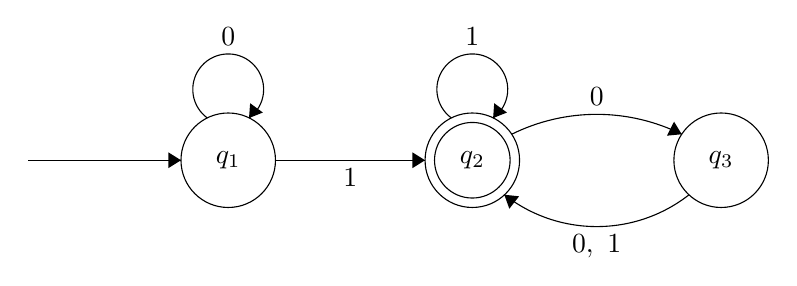
\begin{tikzpicture}[scale=0.2]
	\tikzstyle{every node}+=[inner sep=0pt]
	\draw [black] (16.3,-29.1) circle (3);
	\draw (16.3,-29.1) node {$q_{1}$};
	\draw [black] (31.8,-29.1) circle (3);
	\draw (31.8,-29.1) node {$q_{2}$};
	\draw [black] (31.8,-29.1) circle (2.4);
	\draw [black] (47.6,-29.1) circle (3);
	\draw (47.6,-29.1) node {$q_{3}$};
	\draw [black] (30.477,-26.42) arc (234:-54:2.25);
	\draw (31.8,-21.85) node [above] {$1$};
	\fill [black] (33.12,-26.42) -- (34,-26.07) -- (33.19,-25.48);
	\draw [black] (3.6,-29.1) -- (13.3,-29.1);
	\fill [black] (13.3,-29.1) -- (12.5,-28.6) -- (12.5,-29.6);
	\draw [black] (45.567,-31.289) arc (-51.92551:-128.07449:9.513);
	\fill [black] (33.83,-31.29) -- (34.15,-32.18) -- (34.77,-31.39);
	\draw (39.7,-33.81) node [below] {$0,\mbox{ }1$};
	\draw [black] (14.977,-26.42) arc (234:-54:2.25);
	\draw (16.3,-21.85) node [above] {$0$};
	\fill [black] (17.62,-26.42) -- (18.5,-26.07) -- (17.69,-25.48);
	\draw [black] (19.3,-29.1) -- (28.8,-29.1);
	\fill [black] (28.8,-29.1) -- (28,-28.6) -- (28,-29.6);
	\draw (24.05,-29.6) node [below] {$1$};
	\draw [black] (34.297,-27.451) arc (116.3725:63.6275:12.163);
	\fill [black] (45.1,-27.45) -- (44.61,-26.65) -- (44.16,-27.54);
	\draw (39.7,-25.69) node [above] {$0$};
	\end{tikzpicture}
\end{center}

Powyższy automat akceptuje język $ L = \{ w \in \{0,1\}^{*} | w $ zawiera przynajmniej jedną jedynkę i parzystą liczbę zer na końcu $ \} $.

\subsection{Języki bezkontekstowe - gramatyki bezkontekstowe}

W języku naturalnym jakim jest język polski gramatyka ustala zasady poprawnego budowania zdań. Dzięki temu rozmawiające ze sobą osoby są w stanie się zrozumieć. Języki bezkontekstowe są rodziną szerszą niż omówione wcześniej języki regularne. Język bezkontekstowy to taki język formalny, dla którego istnieje niedeterministyczny automat ze stosem, który potrafi zdecydować czy dany łańcuch należy do języka. Równoważnie dla takiego łańcucha musi istnieć gramatyka bezkontekstowa. Gramatyki bezkontekstowe generują napisy poprzez sekwencję przepisywać, która ma strukturę drzewa. Ze względu na strukturę drzewiastą gramatyki bezkontekstowe nadają się bardzo dobrze do opisu syntaktyki języków programowania.

\begin{definicja}
Gramatyka jest bezkontekstowa, gdy wszystkie jej produkcje są postaci $\mathnormal{A \rightarrow \beta}$, gdzie $\mathnormal{A \in V, \beta \in (\sum \bigcup V)^{*}}$
\end{definicja}

\begin{przyklad}
	Gramatyka $G = (\{a,b  \}, {S}, {S \rightarrow aSb | \epsilon }, S) $ generuje język $ \{a^{n}b^{n}\}$ Język wygenerowany przez gramatykę nie jest regularny.
\end{przyklad}

Tak jak wyrażenia regularne mają równoważny z nimi automat - automat skończony, tak gramatyki bezkontekstowe mają swój odpowiednik maszynowy, jest to automat ze stosem. Automat ze stosem to automat skończony, który został wyposażony w dodatkową pamięć w postaci stosu - jest to lista działająca na zasadzie first in, last out. Nowa symbole mogą być dopisywana lub czytane jedynie na wierzchołku listy. Automaty skończone dysponują skończoną pamięcią, niezależną od długości danych wejściowych. W przypadku automatów ze stosem, dysponujemy także nieskończoną pamięcią, dzięki czemu można rozpoznawać szerszą klasę języków. Tą klasą są języki bezkontekstowe.

\begin{definicja}
	Automatem ze stosem nazywamy system $A_{s} = \langle \sum, Q, F, \Gamma, \delta, q_{0}, Z_{0} \rangle $, gdzie:
	\begin{itemize}
		\item $\sum$ - skończony zbiór symboli wejściowych (alfabet)
		\item $Q$ - skończony zbiór stanów
		\item $\Gamma$ - skończony zbiór symboli na stosie (alfabet stosowy)
		\item $q_{0} \in Q$ - wyróżniony stan początkowy
		\item $Z_{0} \in \Gamma$ - symbol początkowy na stosie - wyróżniony symbol stosowy
		\item $F \subseteq Q$ - jest podzbiorem stanów końcowych
		\item $\delta$ - funkcja przejścia
	\end{itemize}
\end{definicja} 

Maszyna będąc w określonym stanie czyta literę słowa wejściowego oraz sprawdza, jaki symbol znajduje się na wierzchołku stosu. Na tej podstawie podejmowana jest decyzja o zmianie stanu, następnie zdejmowany jest element z wierzchołka stosu. Na zdjętym elemencie umieszczane jest słowo złożone z symboli stosowych. 
\begin{twierdzenie}
	Dla dowolnego języka $L \subset \sum^{*}$ następujące warunki są równoważne:
	\begin{itemize}
		\item Język $L$ jest bezkontekstowy
	 	\item Istnieje gramatyka $G$ prawostronnie liniowa taka, że $L = L(G)$ - język $L$ jest generowany przez gramatykę bezkontekstową $G$
		\item Istnieje automat ze stosem $\underline{A_{s}}  = \langle \sum, Q, F, \Gamma, \delta, q_{0}, Z_{0} \rangle$,
		taki że $L = L(\underline{A})$ - to znaczy, że język $L$ jest akceptowany przez $\underline{A}$
	\end{itemize}
\end{twierdzenie}

	\begin{twierdzenie}
		Język $ L \subset \sum^{*} $ jest generowany przez gramatykę bezkontekstową wtedy i tylko wtedy gdy $L$ jest akceptowalny przez automat ze stosem.
	\end{twierdzenie}	
	
	Niech będzie dany automat ze stosem $A= \langle \sum, Q, F, \Gamma, \delta, q_{1}, Z_{0} \rangle$, który rozpoznaje język $L=\{a^{n}b^{n} | n \ge 1 \}$	
	\begin{center}
		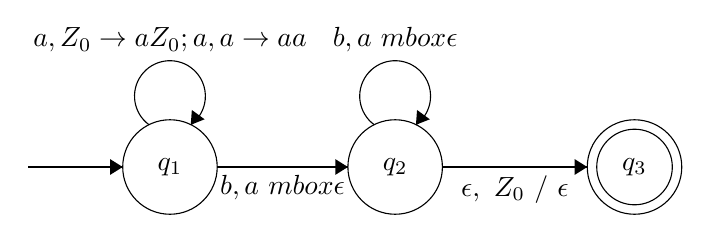
\begin{tikzpicture}[scale=0.2]
		\tikzstyle{every node}+=[inner sep=0pt]
		\draw [black] (21.6,-26.5) circle (3);
		\draw (21.6,-26.5) node {$q_1$};
		\draw [black] (51.1,-26.5) circle (3);
		\draw (51.1,-26.5) node {$q_3$};
		\draw [black] (51.1,-26.5) circle (2.4);
		\draw [black] (35.9,-26.5) circle (3);
		\draw (35.9,-26.5) node {$q_2$};
		\draw [black] (12.6,-26.5) -- (18.6,-26.5);
		\fill [black] (18.6,-26.5) -- (17.8,-26) -- (17.8,-27);
		\draw [black] (20.277,-23.82) arc (234:-54:2.25);
		\draw (21.6,-19.25) node [above] {$a, Z_0 \rightarrow aZ_0; a,a \rightarrow aa$};
		\fill [black] (22.92,-23.82) -- (23.8,-23.47) -- (22.99,-22.88);
		\draw [black] (24.6,-26.5) -- (32.9,-26.5);
		\fill [black] (32.9,-26.5) -- (32.1,-26) -- (32.1,-27);
		\draw (28.75,-27) node [below] {$b,a\mbox{ }\\mbox{ }\epsilon$};
		\draw [black] (38.9,-26.5) -- (48.1,-26.5);
		\fill [black] (48.1,-26.5) -- (47.3,-26) -- (47.3,-27);
		\draw (43.5,-27) node [below] {$\epsilon,\mbox{ }Z_0\mbox{ }/\mbox{ }\epsilon$};
		\draw [black] (34.577,-23.82) arc (234:-54:2.25);
		\draw (35.9,-19.25) node [above] {$b,a\mbox{ }\\mbox{ }\epsilon$};
		\fill [black] (37.22,-23.82) -- (38.1,-23.47) -- (37.29,-22.88);
		\end{tikzpicture}
	\end{center}

	Zapis $a,b \rightarrow c$ oznacza, że maszyna czytając ze słowa wejściowego literę $a$, może zastąpić literę $b$ na wierzchołku ciągiem symboli $c$.




\subsection{Hierarchia Chomsky'ego}
Amerykański językoznawca Noam Chomsky zaproponował cztery typy gramatyk, które maja swoją hierarchę. Hierarchia Choomsky'ego to hierarchia czterech klas języków. Są to języki: regularne, bezkontekstowe, kontekstowe i częściowo obliczalne. Każdej z tych klas przypada jeden rodzaj gramatyki. Odpowiadają im gramatyki: liniowe, bezkontekstowe, kontekstowe i rekurencyjnie przeliczalne. Tym samym klasom odpowiadają cztery różne modele obliczeniowe: automaty skończone, automaty ze stosem, maszyny Turinga (ograniczone liniowo i dowolne). 

\begin{definicja}
	Niech $\mathnormal{G = \langle \sum, V, P, S \rangle}$ będzie dowolną gramatyką.\newline
	\begin{enumerate}
		\item $\mathnormal{G}$ jest typu 1 lub jest gramatyką kontekstową wtedy i tylko wtedy, gdy wszystkie produkcje $\alpha \rightarrow \beta$ spełniają warunek $\mathnormal{|\alpha| \leqslant |\beta|}$
		\item $\mathnormal{G}$ jest typu 2 lub jest gramatyką bezkontekstową wtedy i tylko wtedy, gdy wszystkie produkcje są postaci $\mathnormal{A \rightarrow \beta}$, gdzie $\mathnormal{A \in V, \beta \in (\sum \bigcup V)^{*}}$
		\item $\mathnormal{G}$  jest typu 3 lub jest gramatyką regularną wtedy i tylko wtedy gdy jest prawostronnie lub lewostronnie liniowa.
	\end{enumerate}
\end{definicja}
Poniższy diagram przedstawia graficzną reprezentacje języków formalnych.

\begin{figure}[H]
	\centering
	\includegraphics[width=0.7\linewidth]{hierarchia}
	\caption{Hierarchia języków formalnych}
	\label{fig:hierarchia}
\end{figure}

\begin{definicja}
	Język należy do danej klasy wtedy i tylko wtedy, gdy jest możliwe zbudowanie gramatyki formalnej, która generuje dany język, a której reguły przestrzegają ograniczeń dla danej klasy.
\end{definicja}
 

\section{Gramatyki i muzyka}
Wykorzystanie gramatyki do generowania muzyki charakteryzuje się kilkoma tendencjami. Pierwszą z nich jest określenie jakim rodzajem muzyki ma dana gramatyka się zajmować. Na podstawie rodzaju muzyki należy dokonać charakteryzacji według rodzajów akordów, tempa, linii melodycznej itp. Przykładowo dla muzyki jazzowej można stworzyć produkcje, które będą tworzyły harmoniczne pasujące do siebie akordy bazujące na teorii jazzu i następstwie akordów. 

\subsection{Przykład wykorzystania gramatyk w muzyce}

Jako przykład zostanie przygotowana gramatyka, której celem będzie wygenerowanie prostej melodii bazującej na tonacji C-dur. Na gamę C-dur składają się następujące dźwięki: C, D, E, F, G, A, H. 

\begin{figure}[H]
	\centering
	\includegraphics[width=0.7\linewidth]{c_dur}
	\caption[]{Gama C-dur}
 
	\label{fig:cdur}
\end{figure}

Zapis tonacji C-dur podobnie jak A-moll (A, H, C, D, E, F, G) nie posiada znaków chromatycznych. Tonacje są pokrewne ze sobą. 

Melodia nie powinna przekraczać dwóch oktaw (dwie oktawy: C, D, E, F, G, A, H, C, D, E, F, G, A, H). Metrum melodii czyli czynnik porządkujący ugrupowania rytmicznie za pomocą regularnie powtarzających się akcentów metrycznych wyniesie 4/4 (cztery czwarte). Górna liczba metrum oznacza ile ma być w takcie jednostek miarowych oznaczonych przez liczbę dolną. Przykładowo określenie 2/4 wskazuje, że w jednym takcie mają być dwie ćwierćnuty lub wartości dające w sumie dwie ćwierćnuty. Dolna liczba wskazuje, jaka wartość nutowa jest podstawą miary taktowej. Jednostką miarową może być cała nuta, półnuta, ósemka, szesnastka i trzydziestodwójka. Aby utworzyć melodię kolejność nut musi być ułożona w taki sposób aby utwór był przyjemny dla ucha. Jeżeli nuty zostaną użyte w sposób losowy melodia nie będzie brzmiała dobrze.

\begin{przyklad}
	Rozważmy gramatykę $\mathnormal{G = \langle \sum, V, P, S \rangle}$ gdzie:
	\begin{itemize}
		\item $ \sum = \{ n.k; n \in \langle 0, 87 \rangle, k \in \langle 1, 3 \rangle \} $ - wyrażenie $n.k$ będzie rozpatrywane jako nuta gdzie $n$ oznaczać będzie wysokość nuty, a $k$ długość trwania  dźwięku 1 - cała nuta , 2 - półnuta, 3 - ćwierć nuta. 
		\item $V = \{ S, Beg, Mid, End\}$
		\item Zbiór produkcji $P$ jest następujący: 
		
		$\mathnormal{S \rightarrow Beg\ Mid\ End\ }$\\
		$\mathnormal{Beg \rightarrow 47'1\ 49'1\ 51'1\ 52'1\ }$\\
		$\mathnormal{Beg \rightarrow 52'2\ 56'2\ 59'2\ 57'2\ }$\\
		$\mathnormal{Beg \rightarrow Beg\ 52'2\ 54'2\ 56'2\ 54'2\ Mid\ }$\\
		$\mathnormal{Beg \rightarrow 47'1\ 49'1\ 51'1\ 52'1\ 54'3\ End\ }$\\
		$\mathnormal{Mid \rightarrow Beg\ 52'2\ 56'2\ End\ }$\\
		$\mathnormal{Mid \rightarrow 54'2\ 56'1\ 54'1\ 52'2\ 47'2\ }$\\
		$\mathnormal{Mid \rightarrow Mid\ 47'2\ 52'2\ 56'1\ 57'1\ 56'1\ 52'1\ Beg\ }$\\
		$\mathnormal{Mid \rightarrow 56'2\ 52'1\ 54'1\ 56'2\ }$\\
		$\mathnormal{End \rightarrow Mid\ Beg\ 54'2\ 51'2\ 52'3\  }$\\
		$\mathnormal{End \rightarrow 52'2\ 52'2\ 51'2\ 52'3\ }$\\
		$\mathnormal{End \rightarrow Beg\ 52'2\ 54'2\ 52'3\ End\ }$\\
		$\mathnormal{End \rightarrow 52'4\ }$\\
		$\mathnormal{End \rightarrow 42'2\ 40'3\ }$\\
		$\mathnormal{End \rightarrow 49'1\ 47'1\ 49'1\ 51'1\ 52'3\ End\ }$\\
	\end{itemize}
\end{przyklad}

Za pomocą języka Python można zautomatyzować proces wyprowadzeń. W tym celu będzie pomocna biblioteka nltk, która służy  do pracy z przetwarzaniem języka naturalnego. 

	\begin{lstlisting}[caption={Generowanie wyprowadzeń z gramatyki bezkontekstowej},captionpos=b]
	from nltk import CFG
	from nltk.parse.generate import generate
	import re
	from music21 import *
	notes = ['C', 'C#', 'D', 'D#', 'E', 'F', 'F#', 'G', 'G#', 'A', 'A#', 'B']
	num_notes = 127
	num_octaves = 10
	octave_count = 0
	num_to_note = dict()
	
	for i in range(0, num_notes+1):
	# print "{} {} {}".format(i, octave_count, notes[i%len(notes)])
	num_to_note.update({str(i): notes[i % len(notes)]+str(octave_count)})
	if i % 12 == 11:
	octave_count += 1
	
	gramma = """
	S -> Beg Mid End 
	Beg -> '47.1 49.1 51.1 52.1'
	Beg -> '52.2 56.2 59.2 57.2'
	Beg -> Beg '52.2 54.2 56.2 54.2' Mid
	Beg -> '47.1 49.1 51.1 52.1 54.3' End
	Mid -> Beg '52.2 56.2' End
	Mid -> '54.2 56.1 54.1 52.2 47.2'
	Mid -> Mid '47.2 52.2 56.1 57.1 56.1 52.1' Beg 
	Mid -> '56.2 52.1 54.1 56.2'
	End -> Mid Beg '54.2 51.2 52.3' 
	End -> 52'2 52'2 51'2 52'3
	End -> Beg '52.2 54.2 52.3' End
	End -> '52.4'
	End -> '42.2 40.3'
	End -> '49.1 47.1 49.1 51.1 52.3' End
	"""
	environment.set("musescoreDirectPNGPath",     "/usr/bin/musescore")
	environment.set("musicxmlPath",     "/usr/bin/musescore")
	environment.set("midiPath",     "/usr/bin/lilypond")
	
	conv = converter.subConverters.ConverterLilypond()
	
	grammar = CFG.fromstring(gramma)
	track_array = []
	for track in generate(grammar, n=5, depth=3):
	track_array.append(' '.join(track))
	print (track)
	
	tracks_notes = []
	
	for tr in track_array:
		s1 = stream.Stream()
		for n in re.findall(r'\S+', tr):
		s1.append(note.Note(num_to_note.get(str(n.split('.')[0])), quarterLength=int(n.split('.')[1])))
		tracks_notes.append(s1)
 
	
	
	for i, k in enumerate(tracks_notes):
		print(k)
		conv.write(k, fmt='lilypond', fp='/mnt/c/Users/Lukasz/MGR_Code/Grammar/examples/' + str(i), subformats=['png', 'midi'])	
	\end{lstlisting}	
	Do powyższego przykładu został stworzony interfejs graficzny. Za pomocą interfejsu można wygenerować przykładowe melodie.
	\begin{figure}[H]
		\centering
		\includegraphics[width=0.5\linewidth]{grammar_parser_gui}
		\caption{Interfejs aplikacji}
		\label{fig:grammarparsergui}
	\end{figure}
	
	Interfejs pozwala na wprowadzenie ilości wyprowadzeń oraz głębokości, która jest istotna przy procesie wyprowadzania słów. Zbyt duża głębokość prowadzi do zapętlenia. Po ustaleniu odpowiednich liczb należy wcisnąć przycisk "Generuj".
	
	\begin{figure}[H]
		\centering
		\includegraphics[width=0.7\linewidth]{grammar_parser_gui_results}
		\caption{Wyniki dla głębokości równej 4 oraz liczbie iteracji równej 3}
		\label{fig:grammarparserguiresults}
	\end{figure}

	Po pomyślnym wyprowadzeniu słów program wyświetla wyniki w nowym oknie. 
	



\subsection{Programy wykorzystujące gramatyki}

$\textbf{MusicMachine.io}$ - system stworzony przez Johna Leszczynskiego. Jest to przewodnik, którego celem jest akceptowanie sekwencji nut, które będą spełniały zasady stylu Cantus Firmus. Zasady, które muszą być spełnione to:

\begin{itemize}
	\item sekwencja musi się składać z co najmniej 8 nut
	\item w sekwencji musi wystąpić punk kulminacyjny - jedna nuta musi być wyższa niż pozostałe
	\item koniec sekwencji musi skończyć się na tonice (nuta zaczynająca)
	\item akceptowane interwały to: sekundy wielkie, sekundy małe, tercje, seksty oraz kwarty czyste, kwinty i oktawy
\end{itemize}

Autor oparł swój system na bibliotece napisanej w JavaScript counterpoint (John Jeszczynski jest również autorem tej biblioteki). Interfejs aplikacji jest dostępny pod adresem http://musicmachine.io.


\begin{figure}[H]
	\centering
	\includegraphics[width=0.7\linewidth]{music_machine_gui}
	\caption{Interfejs aplikacji musicmachine}
	\label{fig:musicmachinegui}
\end{figure}

Interfejs musicmachine podaje listę możliwych nut po każdym kroku. Jeżeli sekwencja wybranych nut jest zgodna z zasadami Cantus Firmus to jest akceptowana przez gramatykę umieszczoną w bibliotece. Biblioteka counterpoint wykorzystuje bibliotekę GrammarGraph. Biblioteka GrammarGraph pozwala na stworzenie gramatyki bezkonetkstowej, a następnie pozwala na wyprowadzanie słów z wcześniej zadanej gramatyki oraz potrafi zdecydować czy jakieś wyprowadzenie rzeczywiście pochodzi z gramatyki, która została zadana.

\begin{przyklad}
	Przykład gramatyki zbudowanej w oparciu o temat z Sonaty Księżycowej:
	\begin{lstlisting}[caption={}, captionpos=b]
	var jupiterGrammar = {
	     InfinitePhrase: [ 'JupiterTheme InfinitePhrase',
	         'SecondMotive InfinitePhrase' ],
	     JupiterTheme: [ '2  3  -2' ],
	     SecondMotive: [ '4  StepDown' ],
	     StepDown: [ '-2',
	         '-2  StepDown']
	}
	\end{lstlisting}
	W powyższej gramatyce można wyróżnić symbole terminalne na które składają się: 2, 3, -2, 4. Symbole terminalne oznaczają odległość między nutami - interwały. W skład symboli nie-terminalnych wchodzą: InfinitePhrase, JupiterTheme, SecondMotive, StepDown. Definicje rekurencyjne w gramatyce sprawiają, że długość wyprowadzanego słowa może być nieskończona. 
	
\end{przyklad} 

Gramatyka użyta w aplikacji musicmachine.io wygląda następująco:

\begin{lstlisting}
var upOnly = {

	// designed to be an infinite phrase
	UpPhrase: ['UpLeap DownStepPhrase UpPhrase',
	'UpStepPhrase DownPhrase'],
	
	// all choices must be prepared for a potential down leap in downphrase
	UpStepPhrase: ['Up2Phrase',
	'Up3Phrase',
	'UpLeapForwardPhrase'],
	
	// after 2, can reverse direction or continue up 2 or 3
	Up2Phrase: ['2',
	'2 Up2Phrase',
	'2 Up3Phrase'],
	
	// after 3, can reverse direction or continue up 2
	Up3Phrase: ['3',
	'3 Up2Phrase'],
	
	// up leap must be recovered with down step
	// prepare for a potential downard leap by adding another UpPhrase
	UpLeapForwardPhrase: ['2 UpLeapForward DownStepPhrase UpPhrase'],
	
	// allowed up leaps after already moving a second up
	UpLeapForward: ['4', '5'],
	
	// allowed leaps at the beginning or after a direciton change
	UpLeap: ['4', '5', '6', '8']
}
\end{lstlisting}

Symbole terminalne: 2, 3, 4, 5, 6, 8, oznaczają odległości od nut - interwały. Symbole nie-terminalne: UpPhrase, UpStepPhrase, Up2Phrase, Up3Phrase, UpLeapForwardPhrase, UpLearForward, UpLeap, DownStepPhrase, DownPhrase. Reguły obowiązują w dwóch kierunkach, dolnym i górnym. Gramatyka została zdefiniowana tylko w jednym kierunku, ponieważ kierunek przeciwny można uzyskać zamieniając symbol terminalny na przeciwny. Po każdym wyborze nuty sprawdzane jest czy sekwencja jest prawidłowa z wszystkimi zasadami Cantus Firmus. Za sprawdzanie odpowiedzialna jest poniższa funkcja:

\begin{lstlisting}
	this.isValid = function () {
		var cf = this.cf()
	
		// is it long enough
		if (cf.length < MIN_CF_LENGTH || cf.length > MAX_CF_LENGTH) {
			return false
		}
	
		// is last note tonic?
		if (Pitch(cf[cf.length - 1]).pitchClass() !== guide.tonic()) {
			return false
		} else if (Pitch(cf[0]).pitchClass() === guide.tonic()) {
		// if first note is tonic, last note should end in the same octave
		// if first note is not tonic, this is probably a first species counterpoint
			if (cf[0] !== cf[cf.length - 1]) {
				return false
			}
		}
	
		// is the penultimate note scale degree 2 or possible 7?
		if (intervalSize(cf[cf.length - 2], cf[cf.length - 1]) !== 2) {
			return false
		}
		
		// is there a unique climax (highest note is not repeated)?
		var sorted = sortPitches(cf)
		if (sorted[sorted.length - 1] === sorted[sorted.length - 2]) {
			return false
		}
		
		return true
	}
\end{lstlisting}

Poniżej pokazane zostały dwa przykłady sekwencji, w których jeden jest sekwencją, która spełnia zasady Cantus Firmus, a drugi nie. Prawidłowa sekwencja jest podświetlona na zielono.

\begin{figure}[H]
	\centering
	\includegraphics[width=0.7\linewidth]{music_machine_correct}
	\caption{Prawidłowa sekwencja CantusFirmus}
	\label{fig:musicmachinecorrect}
\end{figure}

\begin{figure}[H]
	\centering
	\includegraphics[width=0.7\linewidth]{music_machine_error}
	\caption{Nieprawidłowa sekwencja}
	\label{fig:musicmachineerror}
\end{figure}

Przykład wyprowadzenia melodii, która jest zgodna z zasadami stylu Cantus Firmus bezpośrednio z wykorzystaniem biblioteki:

\begin{lstlisting}[caption={}, captionpos=b]
var CantusFirmus = require('counterpoint').CantusFirmus
var cantus = new CantusFirmus('G major')
cantus.choices()    => ['G']
cantus.addNote('G4')

cantus.choices()    => [ 'A4', 'B4', 'C5', 'D5', 'E5', 'G5',
'F#4', 'E4', 'G3', 'B3', 'C4', 'D4' ]

cantus.addNote('E5')
cantus.choices()    => [ 'D5', 'C5' ]   

cantus.addNote('D5')
cantus.choices()    => [ 'E5', 'F#5', 'G5', 'A5', 'B5',
'C5', 'B4', 'G4', 'A4' ]
cantus.addNote('F#5')
cantus.choices()    => [ 'G5', 'E5', 'F#4', 'A4', 'B4' ]

cantus.addNote('G5')
cantus.choices()    => [ 'A5', 'B5', 'F#5', 'E5', 'G4', 'B4', 'C5', 'D5' ]

cantus.addNote('B4')
cantus.choices()     => [ 'C5', 'D5' ]
cantus.addNote('C5')
cantus.addNote('A4')

cantus.choices()     => [ 'B4', 'D5', 'E5', 'F#5', 'A5', 'G4' ]
cantus.addNote('G4')

console.log(cantus.print())

G5                  o
F#5             o
E5      o
D5          o
C5                          o
B4                      o
A4                              o
G4  o                               o
	   G4  E5  D5  F#5 G5  B4  C5  A4  G4

\end{lstlisting}

$\textbf{Kulitta}$ - framework napisany w Haskellu przez Donya Quick przeznaczony do automatycznego i algorytmicznego komponowania muzyki. System używa generatywnych gramatyk do tworzenia abstrakcyjnej struktury muzycznej, która jest następnie stopniowo ulepszana za pomocą matematycznych modeli harmonii. Kolejno specyficzne dla stylu algorytmy zamieniają harmonie w konkretny rodzaj muzyki np. chorał, jazz czy bossa nova.

\begin{figure}[H]
	\centering
	\includegraphics[width=0.7\linewidth]{kulitta_diagram}
	\caption{Struktura framerowka Kulitta}
	\label{fig:kulittadiagram}
\end{figure}
 
Kulitta korzysta ze specjalnego rodzaju gramatyk jakim są Probabilistic Temporal Graph Grammars (PTGG). PTGG są podobne do gramatyk bezkontekstowych, umożliwiają równoczesne generowanie harmonicznej i metrycznej struktury za pomocą sparametryzowanego alfabetu.  

\begin{figure}
	\centering
	\includegraphics[width=0.7\linewidth]{ptgg}
	\caption{Przykład PTGG nad symbolami funkcji akordowych, tonika (T),
		dominanta (D) i subdominanta(S), sparametryzowana przez czas trwania jako indeks górny.
		Przedstawione prawdopodobieństwa produkcyjne pochodzą z głównej części potrzebnej do generowania chorałów}
	\label{fig:ptgg}
\end{figure}
\chapter{Sieci Neuronowe}

\section{Wprowadzenie}

Temat sieci neuronowych oraz uczenia maszynowego obecnie stanowi przedmiot zainteresowania wielu osób. Współczesne sieci neuronowe są kamieniem milowym w dziedzinie sztucznej inteligencji. Dzięki uczeniu maszynowemu mamy dostęp do solidnych filtrów anty spamowych, programów do rozpoznawania tekstu i głosu, szybkich i niezawodnych wyszukiwarek internetowych oraz w niedalekiej przyszłości bezpiecznymi i wydajnymi samochodami autonomicznymi. Aby poznać intuicję uczenia maszynowego postawmy problem, który polega na zbudowaniu klasyfikatora, który to na podstawie rysunku lub filmu będzie potrafił rozpoznawać obiekty. Sieci wielowarstwowe służą do budowania warstw interpretacyjnych. Każda warstwa wykorzystuje dane z poprzedniej warstwy.

\begin{figure}[H]
	\centering
	\includegraphics[width=0.5\linewidth]{deep_network}
	\caption{Schemat wielowarstwowej sieci neuronowej $\pagenote{Ian Goodfellow, Yoshua Bengio, Aaron Couville, \textit{Deep Learning Systemy uczące się}, PWN, Warszawa 2018}$}
	\label{fig:deepnetwork}
\end{figure}

Taka architektura została zaproponowana, ponieważ komputer nie potrafi zrozumieć znaczenia surowych danych reprezentowanych jako zbiór pikseli. Początkowe dane trafiają do widocznej warstwy początkowej, następnie warstwy ukryte wyciągają z obrazu cechy. Mając zbiór pikseli pierwsza warstwa ukryta może zidentyfikować krawędzie na podstawie porównań jasności sąsiednich pikseli. Kolejna warstwa, która zna krawędzie występujące na obrazku może zidentyfikować narożniki i rozszerzone kontury. Kolejna warstwa mając opisy z poprzednich warstw może wykryć całe fragmenty określonych obiektów. Opis obrazu w postaci kategorii: krawędzie, narożniki, obiekty i części może być wykorzystany do rozpoznania obiektów znajdujących się na obrazie. Podobny model można zastosować w przypadku generowania muzyki bądź wykrywania gatunku muzycznego na podstawie utworu. Utwór muzyczny posiada wiele cech: metrum, wysokość dźwięku, długość dźwięku. W takim przypadku każda warstwa sieci neuronowej może być odpowiedzialna za charakteryzację każdej cechy.

\section{Model sztucznego neuronu}

Sieci neuronowe nie są nową technologią. Pierwsze pomysły aby wykorzystać zasadzę działania ludzkich neuronów w modelach matematycznych pojawiły się w latach 40 ubiegłego wieku. Biologiczny neuron jest aktywowany na podstawie danych wejściowych. Dane pochodzą z kilku powiązanych neuronów wejściowych. Neurony za pomocą dendrytów rejestrują pozytywne i negatywne informacje wyjściowe z innych neuronów i kodują je za pomocą impulsów elektrycznych przesyłanych przez akson. Następnie akson rozdziela się i dociera do setek tysięcy dendrytów innych neuronów. Pomiędzy aksonem, a wejściowymi dendrytami następnych neuronów znajduje się synapsa. Synapsa odpowiada za przekształcanie impulsów elektrycznych na chemiczne sygnały wpływające na dendryt następnego neuronu. Wynik uczenia jest kodowany przez same neurony. Neurony przesyłają wiadomości aksonami wtedy, gdy poziom pobudzenia jest wystarczająco wysoki. 
\begin{figure}[H]
	\centering
	\includegraphics[width=0.7\linewidth]{schemat_neuronu}
	\caption{Schemat biologicznego neuronu \pagenote{\texttt{https://sebastianraschka.com/Articles/2015\_singlelayer\_neurons.html}}}
	\label{fig:schematneuronu}
\end{figure}

Warren McCulloch i Walter Pitts w roku 1943 opracowali model sztucznego neuronu, nazwali go $\textbf{MCP}$ od McCullock-Pitts$\pagenote{W. S. McCulloch and W. Pitts. A logical calculus of the ideas immanent in nervous activity. The bulletin of mathematical biophysics, 5(4):115–133, 1943}$ swoje wyniki opisali w dziele o nazwie \textit{A Logical Calculus of the Ideas Immanent in Nervous Activity}. Naukowcy przestawili neuron w postaci prostej bramki logicznej z binarnym wyjściem. Za pomocą neuronów MCP można zbudować prostą sieć neuronową, która realizuje funkcje logiczne AND i OR. Klika lat później w roku 1953 amerykański uczony Frank Rosenblatt zaproponował sztuczną sieć neuronową$\pagenote{F. Rosenblatt. The perceptron, a perceiving and recognizing automaton Project Para. Cornell Aeronautical Laboratory, 1957}$, którą nazwał perceptronem. Sieć zaprojektowana przez Rosenblatta mogła nauczyć się rozpoznawania ograniczonej klasy wzorców. Algorytm uczenia perceptronu polega na doborze wag dla sygnałów wejściowych w celu narysowania liniowej granicy decyzji, która pozwala nam rozróżnić dwie liniowo rozłączne klasy. Dane wejściowe są otrzymywane za pośrednictwem odpowiedników dendrytów, następnie obliczana jest suma z uwzględnieniem wag. Jeżeli dane wyjściowe przekroczą określony próg, a wejście hamujące nie jest aktywne to neuron wygeneruje wartość pozytywną. Jeżeli wejście hamujące jest aktywne, dane wyjściowe są hamowane, oznacza to że dane są niepoprawne. Model sztucznego neuronu jest modelem liniowym w przestrzeni n-wymiarowej gdzie n to liczba wejść neuronu, a wejścia powiązane są ze współczynnikami. 

\begin{figure}[H]
	\centering
	\includegraphics[width=0.5\linewidth]{perceptron_latex}
	\caption{Model perceptronu}
	\label{fig:neuron}
\end{figure}

Wejście $a$ można opisać za pomocą równania $a = w_{1}x_{1} + ... + w_{m}x_{n}$, gdzie:

\[
\textbf{w} = 
\begin{bmatrix}
w_{1} \\ \dots \\ w_{n}
\end{bmatrix},
 \textbf{x} =
\begin{bmatrix}
x_{1} \\  \dots \\ x_{n}
\end{bmatrix}
\]

Mając zdefiniowany wektor wejść oraz wag powyższe równanie można rozszerzyć do:

\begin{gather*} 
a = w_{0}x_{0} + w_{1}x_{1} + ... + w_{n}x_{n} = \textbf{w}^{T}\textbf{x}
\end{gather*}



Opis modelu:
\begin{itemize}
	\item Każde wejście $x_{n}$ posiada wagę $w_{n}$. Wartość wejścia jest mnożona przez wartość wagi.
	\item Obliczana jest suma $\sum w_{i}x_{i}$
	\item Funkcja aktywacji $\phi(a)$ pobudza neuron w zależności od zwróconej wartości (większej od granicy $\theta$ lub nie).
\end{itemize}

Prościej, model sztucznego neuronu można opisać za pomocą dwóch równań:
\begin{itemize}
	\item $a  = \sum_{j=1}^{n} w_{j}x_{j}$
	\item $y  = \phi (u + w_{0}) $
\end{itemize}

Funkcja aktywacji $\phi$ jest funkcją progową, to znaczy, że wyjście funkcji jest równe 1 dla dowolnej wartości wejściowej nie większej niż $\theta$.


\[
\phi(a)= 
\begin{cases}
1, & \text{if }  a \geq \theta \\
-1,              & \text{w przeciwnym wypadku}
\end{cases}
\]

Model perceptronu ma trzy ważne cechy:
\begin{itemize}

\item	Do sumy dodawany jest błąd systematyczny (ang. bias) uwzględniany przy sprawdzaniu progu. Ma to kilka celów. Po pierwsze, pozwala uwzględnić błąd statystyczny występujący w neuronach wejściowych. Po drugie, umożliwia standaryzację progów z użyciem wartości (na przykład zera) bez utraty ogólności.

\item	W perceptronie wagi wartości wejściowych mogę być niezależne od siebie i ujemne. Oznacza to dwie ważne rzeczy. Po pierwsze, neuronu nie trzeba wielokrotnie wiązać z wejściem, aby zwiększyć znaczenie danego wejścia. Po drugie, wejście z dendrytu może mieć wpływ hamujący, jeśli przypisana jest mu ujemna waga.

\item	Opracowanie perceptronu dało początek algorytmom uczącym się optymalnych wag na podstawie zbioru danych wejściowych i wyjściowych
\end{itemize}


\subsubsection{Algorytm uczenia się Perceptronu}   

\begin{enumerate}
	\item  Stwórz wektor wag składający się z liczb z przedziału 0, 1
	\item  Dla każdej wartości treningowej $x^{(i)}$:
		\begin{enumerate} 
			\item Oblicz wartość wyjściową $ \hat{y} $
			\item Zaktualizuj wag
			\end{enumerate}
\end{enumerate}

Wartość wyjściowa $\hat{y}$ to etykieta klasy do której zostało przyporządkowane dane wejście. Aktualizację każdej wagi $w_{j}$ w wektorze wag $\textbf{w}$ można zapisać jako:


\begin{gather*} 
w_{j} := w_{j} + \Delta w_{j}
\end{gather*}

Wartość $\Delta w_{j}$, która służy do aktualizacji wag obliczana jest według tak zwanej reguły uczenia perceptronu:

\begin{gather*} 
\Delta w_{j} = \eta ( y^{(i)} - \hat{y}^{(i)} ) x_{j}^{(i)}
\end{gather*}

Gdzie $\eta$ to pewna stała uczenia, zwykle wybierana z przedziału pomiędzy 0, 1. $y^{(i)}$ jest etykietą  i-tej próbki szkoleniowej, a $\hat{y}^{(i)}$ jest przewidywaną etykietą klasy. Wszystkie wagi w wektorze wagowym są aktualizowane jednocześnie. 

\begin{definicja}
	Proces uczenia neuronu wymaga zdefiniowania hipotezy $h_{\theta}$. Dla danych wejściowych $x^{(i)}$ predykcje można opisać za pomocą $h_{\theta}(x^(i))$
\end{definicja}

\begin{definicja} 
	Funkcja straty:
	 \begin{equation}
		  L:(z,y) \in \mathbb{R} \times Y \rightarrow L(z,y) \in \mathbb{R}
	 \end{equation}
	  Funkcja przyjmuje dane wejściowe $z$ oraz ich przewidywaną wartość $y$. Funkcja zwraca liczbę mówiącą o tym jak bardzo dane $z$ oraz $y$ różnią się między sobą.
\end{definicja}

\begin{definicja}
	Funkcja kosztu $J$ jest używana do zebrania informacji na temat efektywności procesu uczenia się. Do jej zdefiniowana używana jest funkcja straty $L$.
	\begin{equation}
		J(\theta) = \sum_{i=1}^{m} L(h_{\theta} (x^{(i)}), y^{(i)})
	\end{equation}
	W uczeniu nadzorowanym występują różne funkcje kosztu. Zostały one pokazane w tabeli poniżej.
	\newline
	\begin{table}[H]
	\bgroup
	\def\arraystretch{1.5}
	\captionof{table}{Zestawienie funkcji kosztu} 
	\centering
	\begin{tabular}{|c|c|c|c|}
		\hline 
		MSE& Strata logistyczna & Utrata zawiasów & Entropia krzyżowa \\ 
		\hline 
		$\frac{1}{2} (y - z)^{2}$ & $log(1 + exp(-yz))$ & $max(0,1 - yz)$ & $- \big[ylog(z) + (1-y)log(1-z) \big] $ \\ 
		\hline 
		 Regresja liniowa&Regresja logistyczna & SVM & Sieci neuronowe  \\ 
		\hline 
	\end{tabular} 
	\egroup
	\end{table}

	Jeżeli funkcja kosztu $J$ jest różniczkowalna do jej minimalizacji można użyć metody największego spadku gradientowego. Celem metody spadku gradientowego jest znalezienie takich wag, które minimalizują funkcję kosztu. Wartość $\frac{1}{2}$ na początku wzoru dodana jest dla ułatwienia obliczeń.
	
\end{definicja}

\begin{twierdzenie}
	Uczenie sieci neuronowej polega na minimalizacji funkcji kosztu.
\end{twierdzenie}

\begin{twierdzenie}
	Jeśli zbiór danych jest liniowo separowalny, a współczynnik szybkości uczenia $ \eta $ jest wystarczająco mały to algorytm uczenia perceptronu jest zbieżny.
\end{twierdzenie}

\begin{twierdzenie}
	Jeśli zbiór danych nie jest liniowo separowalny to algorytm zbiega lokalnie do minimalnego błędu średniokwadratowego.
\end{twierdzenie}


\section{Metoda spadku gradientowego}

Celem algorytmu spadku gradientowego jest minimalizacja funkcji kosztu $J(w)$. Minimalizacja funkcji kosztu pozwala na odpowiedni dobór wag. Ogólnie mówiąc minimalizacja funkcji polega na schodzeniu po jej powierzchni w oparciu o jej nachylenie. Aktualizacja wag polega na wykonaniu kroku w kierunku przeciwnym do gradientu $\nabla J(w)$ funkcji kosztu $J(w)$.
\begin{gather*} 
w := w + \Delta w
\end{gather*}

Gdzie zmiana wagi $\Delta w$ zdefiniowana jest jako:
\begin{gather*} 
\Delta w = - \eta \nabla J(w)
\end{gather*}

gdzie $\eta$ to stała uczenia - szybkość schodzenia w dół. Aby obliczyć gradient funkcji kosztu potrzeba wyliczyć pochodną cząstkową funkcji kosztu dla danej wagi $w_{j}$:

\begin{equation}
\frac{\partial J}{\partial w_{j}} = - \sum ( y^{(i)} - \phi(z^{(i)})) x_{j}^{(i)}
\end{equation}

Zatem reguła aktualizacji wag może wyglądać w następujący sposób:

\begin{equation}
	 \delta w_{j} = -\eta \frac{\partial J}{\partial w_{j}} = \eta \sum_{i} ( y^{(i)} - \phi(z^{(i)})) x_{j}^{(i)}
\end{equation}

\begin{przyklad}
	Dana jest funkcja jednej zmiennej $ y = f(x) = x^{2} - 4x + 2$, funkcja jest ciągła więc do znalezienia jej globalnego minimum można użyć algorytmu spadku gradientowego, rezultat został pokazany poniżej.
	\begin{figure}[H]
		\centering
		\includegraphics[width=0.5\linewidth]{gradient}
		\caption{Metoda spadku gradientowego}
		\label{fig:gradient}
	\end{figure}

	Poniżej wynik działania algorytmu za dużą stałą uczenia $\eta$:
	\begin{figure}[H]
		\centering
		\includegraphics[width=0.5\linewidth]{gradient_wysoki_eta}
		\caption{Za duży współczynnik uczenia}
		\label{fig:gradientwysokieta}
	\end{figure}
	

\end{przyklad}

\begin{przyklad}
	Funkcję wielu zmiennych można również minimalizować za pomocą spadku gradientowego, pod warunkiem, że taka funkcja jest ciągła. Wyniki można obserwować na płaszczyźnie 3D.
\end{przyklad}

\begin{figure}[H]
	\centering
	\includegraphics[width=0.4\linewidth]{1layererror}
	\caption{Przestrzeń błędów dla sieci jednowarstwowej}
	\label{fig:1layererror}
\end{figure}

\begin{figure}[H]
	\centering
	\includegraphics[width=0.4\linewidth]{2layererror}
	\caption{Przestrzeń błędów dla sieci dwuwarstwowej}
	\label{fig:2layererror}
\end{figure}



\section{Wielowarstwowe sieci neuronowe}

Sieci, które składają się przynajmniej z dwóch neuronów muszą mieć określoną architekturę, ponieważ wyniki zwracane przez te neurony mogą być wejściami dla innych neuronów. Takie sieci można podzielić na dwa rodzaje:
\begin{itemize}
	\item skierowane (ang. feed-forward)
	\item rekurencyjne (ang. recurrent)
\end{itemize}

W sieciach wielowarstwowych wyróżnia się podzbiór neuronów akceptujący dane wejściowe, nazywa się je jednostkami wejściowymi oraz podzbiór neuronów, których wyjście jest również wyjściem całej sieci, są to jednostki wyjściowe. Pozostałe neurony nazywa się ukrytymi. Sieci wielowarstwowe są w stanie przeprowadzić nieliniowy podział danych. Dane wejściowe każdej warstwy pochodzą z warstwy poprzedniej, a dane wejściowe poszczególnych warstw są danymi wejściowymi dla warstw następnych. Sieci skierowane są nazywane również sieciami jednokierunkowymi ponieważ związane to jest z tym, że dane płyną tylko w jedną stronę sieci, nie występują w niej cykle. Sieć wielowarstwową można powiązać ze skierowanym grafem acyklicznym opisującym, jak funkcje są ze sobą powiązane. Załóżmy sytuacje, w której mamy trzy funkcje $f^{(1)}, f^{(2)} i f^{(3)}$ połączone w łańcuch, tworząc $f(x) = f^{(3)} (f^{(2)} ( f^{(1)} (x)))$. Sieci wielowarstwowe najczęściej reprezentuje się właśnie w postaci takich struktur łańcuchowych. W takiej strukturze mówimy, że $f^{(1)}$ jest pierwszą warstwą sieci, $f^{(2)}$ to druga warstwa sieci. Całkowita długość łańcucha funkcji daje w wyniki głębokość modelu. Poniżej został przedstawiony model wielowarstwowej sieci neuronowej, który zawiera $(L+1)$-warstw z $D$ wejściami oraz $C$ wyjściami.


\begin{figure}[H]
	\centering
	\includegraphics[width=0.7\linewidth]{multi_layer_neural}
	\caption{Model wielowarstwowej sieci neuronowej}
	\label{fig:multilayerneural}
\end{figure}



Wagę wielowarstwowych sieci neuronowych pokazują następujące ważne twierdzenia:

\begin{twierdzenie}
	Każda funkcja boolowska może być reprezentowana przez sieć z jedną warstwą ukrytą, ale może wymagać wykładniczej liczby jednostek ukrytych.
\end{twierdzenie}

\begin{twierdzenie}
	Każda ograniczona funkcja ciągła może być aproksymowana z dowolnie małym błędem przez sieć z jedną warstwą ukrytą [Cybenko1989; Hornik et al. 1989]
\end{twierdzenie}

\begin{twierdzenie}
	Dowolna funkcja może być aproksymowana z dowolną dokładnością przez sieć z dwoma warstwami ukrytymi [Cybenko 1988]
\end{twierdzenie}

Sieć neuronowa złożona z jednej warstwy ma ograniczenia, ponieważ może tylko realizować problemy liniowo separowalne. Bardzo klasycznym nieliniowym problemem jest funkcja XOR (alternatywa wykluczająca). Funkcja działa na dwóch wartościach bitowych $x_{1}$ i $x_{2}$. Funkcja zwraca 1 wtedy gdy dokładnie jedna z dwóch wartości jest równa 1. Ograniczenia sieci jednowarstwowych opisali Marvin Minsky i Seymour Papert w książce po tytułem Perceptrons: An Introduction to Computational Geometry. W swojej książce przedstawili funkcję XOR jako problem nieliniowy, z którym pojedynczy perceptron lub jednowarstwowa sieć sobie nie poradzi. 

 
	\begin{table}[H]
	\centering
	\begin{tabular}{@{ }c@{ }@{ }c | c@{ }@{ }c@{ }@{ }c@{ }@{ }c@{ }@{ }c}
		p & q &  & p & XOR & q & \\
		\hline 
		0 & 0 &  &  &  0& \\
		0 & 1 &  &  &  1 & \\
		1 & 0 &  & &   1& \\
		1 & 1 &  &  & 0& \\
	\end{tabular}
	\caption{Tabela prawdy dla funkcji XOR} \label{tab:sometab}
	\end{table}
 

Funkcja XOR przedstawiona na wykresie dowodzi, że jej dane wyjściowe nie są liniowo separowalne w przestrzeni dwuwymiarowej. To znaczy, że nie istnieje jedna prosta, która pozwalałaby na rozdzielenie elementów klasy pozytywnej i negatywnej. Punkty można poprawnie rozdzielić przy pomocy więcej niż jednej prostej. Taką możliwość daje architektura sieci wielowarstwowej. Aby skonstruować sieć, która będzie wstanie nauczyć się problemu XOR wystarczy sieć dwuwarstwowa z jedną warstwą ukrytą. Sieć na wejściu przyjmuje dwie wartości, które potrzebne są do obliczenia funkcji XOR. W tak opracowanej sieci każdy węzeł tworzy hiperpłaszczyznę. Wszystkie hiperpłaszczyzny są łączone przez końcowy perceptron. W efekcie otrzymujemy podprzestrzeń, która jest zbiorem wypukłym. Kolejnym ważnym problemem jest odpowiedni dobór wag, które trzeba wyliczyć automatycznie. Wagi powinny być tak dobrane aby można było je wykorzystać do klasyfikowania i prognozowania danych innych niż te pierwotne wejściowe. 

\section{Funkcje aktywacji}

Sieci neuronowe pozwalają na stosowanie szerokiego zakresu funkcji aktywacji. Wybór funkcji aktywacji zależy głównie od tego jaki problem sieć neuronowa powinna rozwiązać. W sieciach wielowarstwowych najczęściej stosowane są funkcje nieliniowe, ponieważ ich nieliniowość jest ważną cechą potrzebną do sprawnego uczenia. Funkcje aktywacje można podzielić na:

\begin{itemize}
	\item nieliniowe
	\item liniowe
	\item skoku jednostkowego (progowa)
\end{itemize}

Ostatni rodzaj funkcji aktywacji jest najbardziej podstawową aktywacji neuronu. Funkcja ta umożliwia otrzymanie na wyjściu sieci informacji postaci TAK - NIE. 

\begin{equation}
f(x)= 
\begin{cases}
0,&  x < 0\\
1,   & x \ge 0
\end{cases}
\end{equation}

\begin{figure}[H]
	\centering
	\includegraphics[width=0.5\linewidth]{stepfunction}
	\caption{Funkcja skoku jednostkowego}
	\label{fig:stepfunction}
\end{figure}

Jeżeli sieć neuronowa ma spełniać zadanie klasyfikatora binarnego (zwraca TAK lub NIE), to funkcja progowa będzie idealną funkcją aktywacji. Problem może pojawić się jeżeli będziemy chcieli wprowadzić więcej klas klasyfikacji. Wtedy jeżeli więcej niż jeden neuron zostanie aktywowany to reszta neuronów automatycznie wyprowadzi 1 z funkcji progowej. Dla większej ilości klas byłoby lepiej, gdy funkcja aktywacji nie była binarna tylko zwracała wartości w postaci np. 20\% dla jednej klasy 50\% dla drugiej i reszta dla ostatniej.

\subsection{Funkcja liniowa}

W przypadku funkcji liniowej sygnał wyjściowy przyjmuje postać:

\begin{equation}
y = cx
\end{equation}

\begin{figure}[H]
	\centering
	\includegraphics[width=0.5\linewidth]{funkcjaLiniowa}
	\caption{Funkcja liniowa}
	\label{fig:funkcjaliniowa}
\end{figure}

W przypadku liniowej funkcji aktywacji aktywacja jest proporcjonalna do sygnału wejściowego neuronu (który jest sumą ważoną).
Takie podejście daje szereg różnych aktywacji, nie ma w tym przypadku aktywacji binarnej. Przy treningu neuronu z liniową funkcją aktywacji może wystąpić problem, ponieważ pochodna dla tej funkcji jest stała. Oznacza to, że gradient nie ma związku z $x$. Jeżeli gradient jest stały to metoda spadku gradientowego również zwróci stały gradient. Jeżeli zostanie użyta wsteczna propagacja błędu to zmiany wprowadzone przez algorytm również będą stałe i nie będą zależne od zmiany wejścia. Bez względu na to z ilu warstw jest zbudowana sieć neuronowa to ostatnia funkcja aktywacji w ostatniej warstwie jest liniową funkcją wejścia pierwszej warstwy.

\subsection{Funkcja sigmoidalna i tanh}

Popularną nieliniową funkcją aktywacji jest funkcja sigmoidalna, której kształt przypomina literę $S$.

\begin{equation}
	f(x) = \frac{1}{1 + e^{-x}}
\end{equation}

\begin{figure}[H]
	\centering
	\includegraphics[width=0.5\linewidth]{sigmoid}
	\caption{Wykres funkcji sigmoidalnej}
	\label{fig:sigmoid}
\end{figure}

Bardzo ważną cechą funkcji sigmoidalnej jest fakt, że jest różnoczkowalna. Warto zauważyć, że pomiędzy wartościami -2 do 2 wartości z osi $y$ są bardzo strome. Każda niewielka zmiana wartości $x$ w tym regionie spowoduje znaczne zmiany wartości $y$. Ten fakt można wykorzystać do doprowadzania wartości $y$ do jednego z końców krzywej. Wyjście funkcji zawsze będzie znajdować się w zakresie $(0, 1)$. W przypadku gdy wartości zwracane przez funkcją będą bardzo blisko krańców krzywej to gradient będzie bardzo mały, na tyle mały że nie będzie można dokonać zmiany wag. W takim przypadku może dojść do sytuacji, że sieć nie będzie w stanie się uczyć lub proces uczenia będzie bardzo wolny. Taki problem określa się mianem znikającego gradientu$\pagenote{\texttt{https://arxiv.org/pdf/1211.5063.pdf}}$.

\\

Kolejną używaną funkcją aktywacji w sieciach neuronowych jest funkcja $\textit{tanh}$:

\begin{equation}
f(x) = tanh(x) = \dfrac{2}{1 + e^{-2x}} - 1
\end{equation}

powyższe równanie można sprowadzić do wcześniej wspomnianej funkcji sigmoidalnej:

\begin{equation}
tanh(x) = 2sigmoid(2x) - 1
\end{equation}

\begin{figure}[H]
	\centering
	\includegraphics[width=0.5\linewidth]{tanh}
	\caption{Wykres funkcji tanh}
	\label{fig:tanh}
\end{figure}

Charakterystyka funkcji $tanh$ jest podobna jak w przypadku funkcji sigmoidalnej. W przypadku funkcji tanh gradient jest znacznie silniejszy niż w przypadku funkcji sigmoidalnej. Również w przypadku funkcji than występuje problem znikającego gradientu. 

\subsection{Funkcja ReLu}

\begin{equation}
	f(x) = max(0, x)
\end{equation}

Funkcja $\textit{Rectified Linear Units}$ jest zalecana do zastosowania w większości jednokierunkowych sieci neuronowych.

\begin{figure}[H]
	\centering
	\includegraphics[width=0.5\linewidth]{relu}
	\caption{Funkcja ReLu}
	\label{fig:relu}
\end{figure}

Funkcja $ReLu$ jest funkcją nieliniową, która zwraca wartości z przedziału $<0, \infty$. Z wykresu funkcji można odczytać, że funkcja $ReLu$ może rzadko aktywować neuron. Dla ujemnych wartości $x$ funkcja zwraca wartość 0, co wyraźnie widać na wykresie w postaci poziomej linii. W przypadku aktywacji ten obszar funkcji $ReLu$ dla gradientu będzie wynosił 0. Oznacza to, że neurony wchodzące w ten obszar przestaną reagować na zmiany. O tym zjawisku mówi się jako o "umieraniu neuronu" lub "problem umierającego ReLu". Ten problem może spowodować sytuacje, że kilka neuronów po prostu umrze i nie będzie reagować przez co część sieci do niczego się nie przyda. Funkcja $ReLu$ jest znacznie mniej kosztowna obliczeniowo niż $tanh$ i $sigmoid$. Warto ja rozważyć w przypadku projektowania głębokiej sieci neuronowej. 

Podsumowując, wymagane cechy funkcji aktywacji to:
\begin{itemize}
	\item ciągłe przejście pomiędzy swoją wartością maksymalną a minimalną (funkcja musi być ciągła)
	\item łatwa do obliczenia i ciągła pochodna
\end{itemize} 


\section{Wsteczna propagacja błędu}

W sieciach jednokierunkowych gdzie na wejściu przyjmowany jest wektor $x$ dane wejściowe podają początkową informację, która przepływa w górę do ukrytych jednostek w każdej sieci, w rezultacie otrzymujemy $\hat{y}$. Jedną z głównych zalet sieci neuronowych jest to, że nie musimy ręcznie podawać wag. Można te wagi wytrenować, czyli znaleźć ich w przybliżeniu optymalny zestaw za pomocą algorytmu wstecznej propagacji błędu. Autorami algorytmu są D. E. Rumelhart, G. E. Hinton,
i R. J. Williams, swoje wyniki opublikowali na łamach prestiżowego magazynu $\textit{Nature} \pagenote{Learning representations by back-propagating errors, D. E. Rumelhart, G. E. Hinton,
	and R. J. Williams, Nature, 323: 6088, strony 533–536, 1986}$  Po mimo tego, że sam algorytm ma ponad 30 lat to jest jednym z najważniejszych algorytmów stosowanych do efektywnego uczenia sieci neuronowych. O samym algorytmie można myśleć jak o wydajnej metodzie, która służy do obliczania pochodnych cząstkowych funkcji kosztu w wielowarstwowych sieciach neuronowych. Problem w wielowarstwowych sieciach polega na tym, że mamy do czynienia z bardzo dużą liczbą współczynników, które trzeba wyznaczyć. W przeciwieństwie do pozostałych modeli funkcja kosztu w sieci wielowarstwowej nie jest wypukła ani gładka w odniesieniu do parametrów. Istnieje więc wiele nierówności w wielowymiarowej przestrzeni, które trzeba zoptymalizować tak aby znaleźć globalne minimum. W algorytmie wstecznej propagacji błędów jest wykorzystywana reguła łańcuchowa, której zadaniem jest obliczenie pochodnej funkcji złożonej.

\begin{fact}
	Algorytm propagacji wstecznej działa dla dowolnego grafu skierowanego bez cykli.
\end{fact}

\begin{twierdzenie}
	Algorytm propagacji wstecznej zbiega lokalnie do minimalnego błędu średniokwadratowego.
\end{twierdzenie}


\begin{equation}
\frac{d}{dx}
\big[ f(g(x)) \big] = \frac{df}{dg} \cdot \frac{dg}{dx}
\end{equation}

	Reguły łańcuchowej możemy użyć do długiej złożonej funkcji, funkcja ta może reprezentować wielowarstwową sieć neuronową. Załóżmy, że sieć składa się z pięciu warstw: $F(x)= f(g(g(u(v(x)))))$. Po zastosowaniu reguły łańcuchowej możemy policzyć pochodne ze wzoru:
	
	\begin{equation}
		\frac{dF}{dx} = \frac{d}{dx}F(x)=\frac{d}{dx}f(g(h(u(v(x))))) = \frac{df}{dg} \cdot \frac{dg}{dh} \cdot \frac{dh}{du} \cdot \frac{du}{dv} \cdot \frac{dv}{dx}
	\end{equation}
	
	W algorytmie wstecznej propagacji wykorzystuje się pochodną funkcji aktywacji. Pochodna informuje o tym czy dla zadanego zestawu wag funkcja aktywacji jest odpowiednio pobudzona. Dzięki temu można dowiedzieć się w którym kierunku i jak bardzo zaktualizować wagi.
	
	Poniżej zostanie przedstawiony proces uczenia wielowarstwowej sieci neuronowej z użyciem algorytmu wstecznej propagacji błędu na przykładzie trójwarstwowej sieci neuronowej o dwóch wejściach i jednym wyjściu. Przepływ w takiej sieci można wyrazić za pomocą listy kroków:
	
	\begin{itemize}
		\item Warstwa wejściowa $Z$  jest wyrażona za pomocą równania $Z = A * W$, gdzie $A$ to macierz danych wejściowych, a $W$ to macierz wag dla danych wejściowych
		\item Iloczyn oby macierzy trafia do funkcji aktywacji $A$, operację można wyrazić za pomocą wzoru $A = \phi(Z))$ - operacja odbywa się w warstwie ukrytej
		\item Wynik funkcji aktywacji trafia do warstwy wyjściowej i jest wymnażany przez macierz wag $Z = A * W$
		\item Obliczone dane w warstwie wyjściowej trafiają do funkcji aktywacji $A = \phi(Z)$, wynik przypisywany jest do $z$
	\end{itemize}

	W taki sposób została dokonana propagacja sygnału przez całą sieć w kierunku od lewej strony do prawej.	W algorytmie wstecznej propagacji błędu błąd jest propagowany z prawej do lewej. Proces zaczyna się od obliczenia błędu w warstwie wyjściowej:
	
	\begin{equation}
	\delta = z - y 
	\end{equation}
	
	Sygnał wyjściowy sieci porównywany jest z oczekiwaną wartością sygnału wyjściowego. Różnica obu wartości nazywana jest sygnałem błędu $\delta$ neuronu warstwy wyjściowej. Neurony, które znajdują się w warstwach ukrytych nie są w stanie bezpośrednio określić swojego błędu, ponieważ nie są znane wartości oczekiwane sygnałów wyjściowych z tych neuronów. Dzięki wstecznej propagacji błędu błąd jest rzutowany wstecz od prawej do lewej strony. Dzięki temu można obliczyć błąd w warstwie ukrytej.
	
	\begin{equation}
	\delta^{(hidden)} = \delta \big( W \big) ^{T} \frac{\partial \phi(Z^{(hidden)}))}{\partial Z ^{(hidden)}}
	\end{equation}
	
	uwzględniając pochodną funkcji aktywacji powyższe wyrażenie można zapisać jako:
	
	\begin{equation}
		\delta^{(hidden)} = \delta \big(W \big)^{T} \big(a^{(h)} \big(1-a^{(h)}\big)\big)
	\end{equation}
	
	W dalszej kolejności trzeba przechować pochodną cząstkową każdego węzła każdej warstwie oraz błąd węzła w następnej warstwie. Należy obliczyć $\delta_{i,j}^{(l)}$ dla każdej próbki ze zbioru treningowego.
	
	\begin{equation}
		\Delta ^{(hidden)} = \delta^{(hidden)} + \big(A^{(input)}\big)^{T} \delta^{(hidden)}
	\end{equation}
	
	\begin{equation}
	\Delta  = \delta + \big(A^{(hidden)}\big)^{T} \delta
	\end{equation}

	Po wyliczeniu spadku gradientowego należy zaktualizować wagi wykonując przeciwny kroku w kierunku gradientu dla każdej warstwy:
	
	\begin{equation}
		W^{(l)} := W^{(l)} - \eta \Delta^{(l)}
	\end{equation}

	Cały proces można przedstawić za pomocą ilustracji poniżej i przedstawić za pomocą listy kroków:
		
	\begin{figure}[H]
		\centering
		\includegraphics[width=0.9\linewidth]{backprop}
		\caption{Ilustracja wstecznej propagacji błędu}
		\label{fig:backprop.png}
	\end{figure}
	Cały proces można sprowadzić do listy kroków:
	\begin{itemize}
		\item Pobierz dane treningowe
		\item Przeprowadź propagacje sygnału w celu obliczenia błędu
		\item Przeprowadź propagację wsteczną aby uzyskać gradienty
		\item Użyj gradientów aby zaktualizować wagi sieci
	\end{itemize}


	\begin{fact}
	Zauważmy, że możemy określić pojęcie epoki jako jeden cykl podczas którego wszystkie obiekty treningowe poprawiają wagi, na koniec wyliczany jest błąd sumaryczny całego zbioru treningowego. Algorytm uczenia zatrzymuje się, kiedy błąd przestaje maleć.
	\end{fact}

	\begin{figure}[H]
		\centering
		\includegraphics[width=0.7\linewidth]{epoki}
		\caption{Proces uczenia sieci polega na minimalizacji błędu}
		\label{fig:epoki}
	\end{figure}
	
	\section{Rekurencyjne sieci neuronowe}

	Rekurencyjne sieci neuronowe (ang. recurrent neural networks, RNN)(Rumenlhart 1986) to rodzina sieci neuronowych służąca do pracy z danymi sekwencyjnymi. Sieci rekurencyjne mają zastosowanie w tłumaczeniu tekstu, rozpoznawaniu obrazu, rozpoznawaniu mowy czy generowaniu muzyki, ponieważ wszystkie te mechanizmy potrzebują do działania sekwencji. Jedną z pierwszych koncepcji systemów uczących się i modeli statystycznych była możliwość współdzielenia parametrów w różnych częściach modelu. Takie podejście pozwala na rozszerzenie modelu i zastosowanie go do przykładów o różnych postaciach. Istnieje klika różnych kategorii przetwarzania danych sekwencyjnych, które można podzielić ze względu na dane wejściowe i wyjściowe. Takiego podziału dokonał Andrej Karpathy, który opisał w artykule \textit{The Unreasonable Effectiveness of Recurrent Neural Networks}\pagenote{\texttt{http://karpathy.github.io/2015/05/21/rnn-effectiveness/}} Rysunek poniżej obrazuje różne zależności między danymi wejściowymi, a wyjściowymi. 
	
	\begin{figure}[H]
		\centering
		\includegraphics[width=0.7\linewidth]{relacje}
		\caption{Zależności pomiędzy wejściem, a wyjściem w rekurencyjnych sieciach neuronowych $\pagenote{Sebastian Raschka, \textit{Python Machine Learning}, Packt Publishing; 1 edition (September 23, 2015), 540}$}
		\label{fig:relacje}
	\end{figure}
	
	W przypadku kiedy dane wejściowe zawierają sekwencje istnieje klika różnych przypadków modeli, które to zwrócą różne wyjścia. Można je podzielić na trzy główne kategorie.
	
	
	\begin{itemize}
		\item Wiele do jednego - Dane wejściowe to sekwencja, wyjście to wektor o stałym rozmiarze. Dla przykładu na wejściu jest fragment tekstu, a na wyjściu jedno słowo np. emocja opisująca fragment tekstu, inny przykład to sekwencja nut na wejściu, a na wyjściu nazwa gatunku muzycznego pasującego do zadanej sekwencji.
		\item Jeden do wielu - Dane wejściowe nie są sekwencją, natomiast dane wyjściowe składają się z sekwencji. Przykład to opisywanie obrazów, wejście to obraz, a na wyjściu opis obrazu.
		\item Wiele do wielu - Dane wejściowe i wyjściowe składają się z sekwencji. Przykład to tłumaczenie jednego języka na inny, generowanie nowego utworu muzycznego na podstawie innego. 
	\end{itemize}

	W książce $\textit{Deep Learning}$ Yan Goodfellow dokonał podobnego podziału:
	
	\begin{itemize}
		\item sieci rekurencyjne, które generują wartości wynikowe w każdym kroku czasowym i mają rekurencyjne połączenia między ukrytymi jednostkami
		\item sieci rekurencyjne, które generują wartości wynikowe w każdym kroku czasowym i mają rekurencyjne połączenia jedynie między wejściem w jednym kroku czasowym, a jednostkami ukrytymi w kolejnym kroku czasowym
		\item sieci rekurencyjne z rekurencyjnymi połączeniami między ukrytymi jednostkami, które odczytują całą sekwencje, a następnie generują jedno wyjście
	\end{itemize}                 
	
		 Innym historycznym przykładem sieci rekurencyjnej jest sieci $\textbf{Elmana }$ (Elman, 1990) - sieć złożona z trzech podstawowych warstw (wejściowej, ukrytej, wyjściowej) oraz dodatkowej warstwy, której połączenia wejściowe są połączeniami wejściowymi warstwy ukrytej.
		 $\textbf{Sieci Jordana }$ posiadają podobną strukturę do sieci Elmana, połączenia wejściowe do warstwy kontekstowej są połączeniami wyjściowymi z warstwy wyjściowej.
		 $\textbf{Sieci Hopfielda }$ nie posiadają wyróżnionych warstw, każdy neuron połączony jest ze wszystkimi neuronami w sieci, poza sobą, neurony nie mają pętli, każda para neuronów ma połączenie symetryczne.

	Rekurencyjną sieć neuronową można przedstawić za pomocą poniższego wzoru, który oblicza sekwencje wektorów $x$ stosując zasadę rekurencji dla każdego kroku czasowego:
	
	\begin{equation}
	h_{t} = f_{W} ( h_{t-1}, x_{t} )
	\end{equation}
	
	\begin{itemize}
		\item $h_{t}$ - nowy stan
		\item $f_{W}$ - funkcja aktywacji z parametrem $W$
		\item $h_{t-1}$ - poprzedni stan
		\item $x_{t}$ - wektor wejścia w kroku czasowym $t$
	\end{itemize}
	
	Powyższy wzór można przedstawić za pomocą schematu:
	
	\begin{figure}[H]
		\centering
		\includegraphics[width=0.2\linewidth]{rnn_model}
		\caption{Schemat rekurencyjnej sieci neuronowej z jedną warstwą ukrytą}
		\label{fig:rnn}
	\end{figure}
	
	Model sieci rekurencyjnej można rozwinąć w czasie, wtedy otrzymamy:
	
 	\begin{figure}[H]
 		\centering
 		\includegraphics[width=0.7\linewidth]{rnn_forward_pass}
 		\caption{Rekurencyjna sieć neuronowa rozwinięta w czasie}
 		\label{fig:rnnforwardpass}
 	\end{figure}
 	
 	 Sekwencja wejściowa $x = (x^{1}, x^{2}, ..., x^{T_{x}})$ jest aplikowana do sieci w $T_{x}$ krokach czasowych. Na wyjściu sieć zwraca sekwencję $y = (y^{1}, y^{2}, ..., y^{T_{x}})$.
	
	Rekurencyjną sieć neuronową można postrzegać jako powtarzanie pojedynczej komórki. Poniższy rysunek opisuje operacje dla pojedynczego kroku czasowego komórki w rekurencyjnej sieci neuronowej.
	
	\begin{figure}[H]
		\centering
		\includegraphics[width=0.7\linewidth]{rnn_cell}
		\caption{Podstawowa komórka w rekurencyjnej sieci neuronowej.}
		\label{fig:rnncell}
	\end{figure}

	 Powyższa komórka na wejściu otrzymuje $x^{t}$ oraz $a^{t-1}$ z poprzedniego ukrytego stanu, na wyjściu komórka zwraca $a^{t}$, wyjście będzie wykorzystane jako wejście do następnej komórki oraz zostanie użyte do predykcji $\hat{y}^{t}$

	Każda krawędź skojarzona jest z macierzą wag. Macierz wag jest niezależna od danego kroku czasowego $t$. Macierze wag, które występują na rysunku powyżej:
	
	\begin{itemize}
		\item $\textbf{\textit{W}}_{ax}$ - macierz wag pomnożona przez wektor wejściowy
		\item $\textbf{\textit{W}}_{aa}$ - macierz wag pomnożona przez stan ukryty
		\item $\textbf{\textit{W}}_{ya}$ - macierz wag pomiędzy warstwą ukrytą, a warstwą wyjściową
	\end{itemize} 
	
	Trening rekurencyjnej sieci neuronowej odbywa się z wykorzystaniem algorytmu \textit{Backpropagation Through Time}\pagenote{Backpropagation Through Time: What It Does and How to Do It (Paul Werbos, Proceedings of IEEE, 78(10):1550-1560, 1990).}. Algorytm bazuje na metodzie spadających gradientów. Jego główną ideą jest to aby całkowity błąd $L$ był sumą wszystkich funkcji błędu w czasie $t=1$ do $t=T$.

	\begin{equation}
		L = \sum_{t=1}^{T} L^{(t)}
	\end{equation}

	Sieci rekurencyjne stosuje się aby zachowywać długotrwałe zależności w czasie. Jednak niesie to ze sobą pewne problemy, ponieważ im więcej danych nagromadzonych w poszczególnych krokach czasowych to istnieje duże ryzyko, że gradienty obliczane z wykorzystaniem algorytmu BPTT będą się gromadzić. Takie zjawisko może doprowadzić do problemu zanikającego gradientu lub jego eksplozji. Problem ten został dokładnie opisany przez R. Pascanu, T. Mikolov, i Y. Bengio w dziele \textit{On the difficulty of training recurrent neural networks}\pagenote{\texttt{https://arxiv.org/pdf/1211.5063.pdf}}.
	
	Na przestrzeni lat zostały opracowane dwa sposoby, które rozwiązują ten problem:
	\begin{itemize}
		\item Truncated backpropagation through time (TBPTT)$\pagenote{\texttt{http://ir.hit.edu.cn/~jguo/docs/notes/bptt.pdf}}$ 
		\item Long short-term memory (LSTM)$\pagenote{\texttt{http://www.bioinf.jku.at/publications/older/2604.pdf}}$
	\end{itemize}
	\subsection{Pamięć Long Short-Term }
	Współcześnie najbardziej efektywne modele sekwencyjne, które stosowane są w praktyce nazywane są bramkowymi sieciami RNN. Do tych modeli zaliczana jest architektura długiej pamięci krótkoterminowej (ang. long short-term memory). Pierwsza koncepcja architektury LSTM została przedstawiona przez dwóch niemieckich naukowców S. Hochreiter'a oraz J. Schmidhuber'a w 1997 $\pagenote{Sepp Hochreiter, Jurgen Schmidhuber, \textit{Long Short-Term Memory}, Neural Computation}$. Głównym blokiem konstrukcyjnym LSTM jest komórka pamięci, która reprezentowana jest przez ukrytą warstwę w rekurencyjnej sieci neuronowej. Sieci rekurencyjne z blokiem LSTM nazywamy sieciami LSTM. Nad poprawieniem pierwotnej koncepcji LSTM pracowało wiele osób przez kilka lat, wyniki poprawek zostały opisane w pracy $\pagenote{In addition to the original authors, a lot of people contributed to the modern LSTM. A non-comprehensive list is: Felix Gers, Fred Cummins, Santiago Fernandez, Justin Bayer, Daan Wierstra, Julian Togelius, Faustino Gomez, Matteo Gagliolo, and Alex Graves.}$ Sieci LSTM zostały zaprojektowane w celu uniknięcia problemu długotrwałej zależności. Trening sieci LSTM pozwala na zapamiętanie długotrwałych zależności pomiędzy danymi wejściowymi, a wyjściowymi wynikami zwracanymi przez sieć. Struktura komórki LSTM może przypominać pamięć komputera, ponieważ może odczytywać, zapisywać i usuwać informacje za pomocą odpowiednich bramek. Komórka decyduje, czy przechować lub usunąć informacje w zależności od przypisanej wagi do informacji. Wagi dobierane są w procesie uczenia, z upływem czasu komórka LSTM dowiaduje się, które informacje są ważne, a które nie. Struktura komórki LSTM została przedstawiona na rysunku poniżej.
	
	\begin{figure}[H]
		\centering
		\includegraphics[width=1.0\linewidth]{lstm_cell}
		\caption{Komórka LSTM}
		\label{fig:lstmcell}
	\end{figure}
	Głównym rdzeniem komórki LSTM jest wyprowadzenie, które na wejściu przyjmuje pamięć z poprzedniego kroku czasowego $c^{\langle t-1 \rangle}$ i zwraca aktualny stan pamięci $c^{\langle t \rangle}$. Komórka posiada trzy wejścia. Pierwsze z nich to wektor $x^{t}$ w kroku czasowym $t$. $a^{\langle t-1 \rangle}$ oznacza wyjście z poprzedniej komórki LSTM. Wcześniej wspomniane $c^{\langle t-1 \rangle}$ to pamięć z poprzedniej jednostki. Symbol $\odot$ zamieszczony na schemacie to iloczyn Hadamarda.
	
	$\newline$
	Komórka LSTM posiada trzy różne typy bramek:
	
	\begin{itemize}
		\item Bramka zapomnienia (ang. forget gate) pozwala komórce pamięci na wymazanie pamięci. Wektory wejściowe po wymnożeniu przez wagi trafiają do sigmoidalnej funkcji aktywacji. Funkcja aktywacji zwraca wektor, którego elementy są z zakresu (0, 1). Kolejno wektor jest poddany iloczynowi Hadamarda ze wcześniejszym stanem komórki pamięci  $c^{\langle t-1 \rangle}$. Kluczową rolę pełni wektor zwrócony przez funkcję aktywacji, ponieważ jeżeli jego elementy są bliskie zera to po zastosowaniu iloczynu Hadamarda z poprzednim stanem pamięci spowoduje wymazanie odpowiednich elementów z wektora $c^{\langle t-1 \rangle}$. W przeciwnym wypadku jeżeli wartości wektora z funkcji aktywacji będą bliskie zeru to elementy z wektora $c^{\langle t-1 \rangle}$ zostaną zachowane. Bramka zapomnienia nie była częścią oryginalnej komórki LSTM, została dodana kilka lat później$\pagenote{Learning to Forget: Continual
			Prediction with LSTM, F. Gers, J. Schmidhuber, and F. Cummins, Neural
			Computation 12, 2451-2471, 2000}$.
		
		\item Bramka aktualizacji (ang. update gate) jej zadaniem jest aktualizacja stanu komórki. Podobnie jak w przypadku bramki zapomnienia bramka aktualizacji zwraca wektor z wartościami z przedziału (0, 1). Bramka jest powiązana z funkcją aktywacji jaką jest tangens hiperboliczny. Zadaniem funkcji aktywacji jest obliczenie nowych wartości, które mogą zostać wstawione do stanu komórki. Funkcja aktywacji tanh przyjmuje wartości z przedziału (-1, 1) więc otrzymany wektor może zawierać elementy o wartościach ujemnych. Iloczyn Hadmarda dwóch wektorów dodawany jest do stanu pamięci. W wyniku otrzymywany jest wektor $c^{t}$ - zaktualizowany stan pamięci.
		
		\item Bramka wyjścia (ang. output gate) - ostatni element komórki LSTM, który składa się z dwóch komponentów: funkcje aktywacji tanh oraz wyjściową funkcję sigmoidalną. 
		
	\end{itemize}
	
	W pierwszym kroku przepływu danych przez komórkę LSTM dane muszą przejść przez bramkę zapomnienia. W tym kroku bramka decyduje, które informacje mają zostać zapominanie, a jakie zachować. Bramka przyjmuje sekwencję danych $x^{t}$ oraz wektor wyjściowy z poprzedniej komórki $h^{t-1}$. Schemat przepływu został zilustrowany poniżej. Poniżej ilustracja przedstawiająca schemat budowy komórki LSTM.
	
	\begin{figure}[H]
		\centering
		\includegraphics[width=0.7\linewidth]{lstm_forget}
		\caption{Pierwszy krok przepływu informacji przez komórkę LSTM $\pagenote{Jose Portilla, \textit{Complete Guide to TensorFlow for Deep Learning with Python}}$}
		\label{fig:lstmforget}
	\end{figure}
	
	W kolejnym kroku następna bramka decyduje jaką informacje należy zachować. Bramka składa się z dwóch części: funkcji sigmoidalej oraz tanh. W wyniku otrzymywany jest wektor, który jest nazywany wektorem nowych wartości kandydujących
	
	\begin{figure}[H]
		\centering
		\includegraphics[width=0.7\linewidth]{lstm_2_krok}
		\caption{Drugi krok przepływu informacji przez komórkę LSTM $\pagenote{Jose Portilla, \textit{Complete Guide to TensorFlow for Deep Learning with Python}}$}
		\label{fig:lstm2krok}
	\end{figure}

	W kolejnym kroku następuje aktualizacja starego stanu komórki, który jest określony przez $c^{t-1}$. Zaktualizowany wektor $c^{t}$ jest odbierany przez kolejną komórkę LSTM w kolejnym kroku czasowym.

	\begin{figure}[H]
		\centering
		\includegraphics[width=0.7\linewidth]{lstm_3_krok}
		\caption{Trzeci krok przepływu informacji przez komórkę LSTM $\pagenote{Jose Portilla, \textit{Complete Guide to TensorFlow for Deep Learning with Python}}$}
		\label{fig:lstm3krok}
	\end{figure}

	Ostatni krok do zwrócenie wartości $h^{t}$, wartość $h^{t}$ jest wartością przewidywaną przez komórkę LSTM w czasie $t$. Połączenie skierowane do góry może posłużyć jako wejście do kolejnej warstwy ukrytej, znajdującej się bezpośrednio nad aktualną. Połączenie skierowane w prawo, stanowi wejście do następnej komórki LSTM.

	\begin{figure}[H]
		\centering
		\includegraphics[width=0.7\linewidth]{lstm_4_krok}
		\caption{Czwarty, ostatni krok przepływu przez komórkę LSTM $\pagenote{Jose Portilla, \textit{Complete Guide to TensorFlow for Deep Learning with Python}}$}
		\label{fig:lstm4krok}
	\end{figure}
	
	Badania wykazują, że sieci LSTM znacznie szybkiej przychodzi poznawanie długotrwałych zależności, przede wszystkim na sztucznych zbiorach danych, zaprojektowanych do testowania takich możliwości (Bengio et al., 1994; Hochreiter and Schmidhuber, 1997; Hochreiter et al., 2001). Testy odbywają się na specjalnych wymagających zadaniach przetwarzania sekwencji (Graves, 2012	Graves et al., 2013; Sutskever et al., 2014).
	Nie wszystkie warianty komórek LSTM są takie same jak opisane powyżej. W publikacjach opisujących LSTM można znaleźć wiele innych wariantów, które są lekko odbiegają od oryginalnego modelu. Jednym z popularnych odmian LSTM jest dodatek wprowadzony przez Gersa i Schmidhubera (2000), który wzbogaca standardową komórkę LSTM o tzw. peephole connections. Są to dodatkowe połączenia pomiędzy stanem pamięci, a bramkami. Nieco innym wariantem LSTM jest Gated Recurrent Unit (GRU), koncept ten został wprowadzony przez Cho, et al (2014)$\pagenote{\texttt{http://arxiv.org/pdf/1406.1078v3.pdf}}$. Jednostka GRU łączy bramkę zapomnienia oraz bramkę aktualizacji. Połączony jest także stan komórki ze stanem ukrytym. Uzyskany model jest prostszy niż standardowe modele LSTM i jest coraz bardziej popularny. Inne popularne modele to Depth Gated RNNs authorstwa Yao, et al (2015). Zupełnie inne podejście przedstawił Koutnik w 2014 w pracy Clockwork RNN. Greff, et al. (2015) zrobił porównanie wszystkich popularnych wariantów i stwierdził, że wszystkie działają tak samo. Rafał Józefowicz$\pagenote{\texttt{http://proceedings.mlr.press/v37/jozefowicz15.pdf}}$ przetestował ponad dziesięć tysięcy różnych architektur i wskazał, że niektóre z nich działają lepiej od standardowej komórki LSTM w zależności od postawionego problemu. 
	
	\subsection{Rodzaj sieci "Sequence to sequence"}
	
	Modele sekwencyjno-sekwencyjne (seq2seq) (Sutskever i in., 2014, Cho i in., 2014)$\pagenote{\texttt{https://papers.nips.cc/paper/5346-sequence-to-sequence-learning-with-neural-networks.pdf}}$ odniosły bardzo duży sukces w modelowaniu zadań dla rekurencyjnych sieci neuronowych takich jak tłumaczenie tekstu, rozpoznawanie mowy czy synteza tekstu. Starsze systemy tłumaczenia tekstu rozbijały zdanie na słowa i dokonywały tłumaczenia pojedynczych wyrazów bez zachowania kontekstu zdania. W modelu seq2seq jest przetwarzana cała sekwencja wejściowa i dopiero na podstawie jej kontekstu jest produkowane wyjście. W skład takiego modelu wchodzi mechanizm odpowiedzialny za kodowanie i dekodowanie sekwencji.
	
	\begin{figure}[H]
		\centering
		\includegraphics[width=0.7\linewidth]{encoder_decoder}
		\caption{Architektura enkoder - dekoder. Enkoder odpowiedzialny jest za konwersje zdania źródłowego na wektor "znaczeniowy", który jest przekazywany przez dekoder w celu procesu tłumaczenia.$\pagenote{\texttt{https://github.com/tensorflow/nmt}}$ }
		\label{fig:encoderdecoder}
	\end{figure}

	\begin{figure}[H]
		\centering
		\includegraphics[width=0.8\linewidth]{seq2seq3}
		\caption{Przykład architektury enkoder-dekoder, której zadaniem jest przetłumaczenie zdania "I am a student" na język francuski "Je suis étudiant". Specjalny znacznik "$<s>$" oznacza rozpoczęcie dekodowania, "$</s>$" oznacza zatrzymanie dekodowania. $\pagenote{\texttt{https://github.com/tensorflow/nmt}}$ }
		\label{fig:seq2seq3}
	\end{figure}
	\begin{figure}[H]
		\centering
		\includegraphics[width=0.8\linewidth]{seq2seq2}
		\caption{Inny przykład architektury seq2se2 zastosowanej do automatycznej odpowiedzi na wiadomości e-mail}
		\label{fig:seq2seq2}
	\end{figure}		
	Muzyka oparta jest na sekwencjach, gdzie kolejny zestaw sekwencji do odegrania zależy od poprzedniego zestawu sekwencji. Model seq2seq może zostać wykorzystany z powodzeniem do wygenerowania nut na podstawie nauczonych sekwencji.	
	\subsection{Rodzaj sieci "Character RNN"}
	Jednym z przykładów sieci operującej bezpośrednio na znakach jest model Character RNN, który został opracowany przez Andreja Karpathego$\pagenote{\texttt{http://karpathy.github.io/2015/05/21/rnn-effectiveness/}}$. Zadaniem sieci po wytrenowaniu jest przewidywanie następnego znaku biorąc pod uwagę sekwencję poprzednich znaków. Taki model można zastosować do generowania muzyki pod warunkiem, że dane wejściowe będą zapisane w formacie tekstowym. Jednak w przeciwieństwie do modelu seq2seq character rnn nie jest w stanie zachować dłużej frazy, ponieważ operuje bezpośrednio na znakach, a nie na sekwencjach. Schemat działania modelu został zilustrowany poniżej.
	
	\begin{figure}[H]
		\centering
		\includegraphics[width=0.5\linewidth]{char_rnn}
		\caption{Schemat modelu Char RNN $\pagenote{\texttt{http://cs231n.stanford.edu/slides/2017/cs231n\_2017\_lecture10.pdf}}$}
		\label{fig:charrnn}
	\end{figure}
	
	Rysunek powyżej ilustruje przykład, w którym rekurencyjna sieć neuronowa uczy się następstwa znaków w wyrazie $\textit{hello}$. Każdy ze znaków jest kodowany za pomocą metody one hot encoding$\pagenote{\texttt{https://machinelearningmastery.com/why-one-hot-encode-data-in-machine-learning/}}$. W pierwszym kroku czasowym dla znaku h zostało przypisane zaufanie wynoszące 1.0, dla kolejnej litery h zaufanie wynosi 2.2, dla e -3.0 oraz l 4.1. W wyrazie hello po literze h występuje litera e, więc sieć powinna zwiększyć zaufanie do tej litery i zmniejszyć do innych. Aby obliczyć w którym kierunku dostosować wagi dla każdej z liter stosuje się algorytm propagacji wstecznej. Cały proces powtarzamy dopóki prognozy sieci będą zgodne z danymi treningowymi. Model ten można przedstawić jako pewne zadanie klasyfikacji, w którym klasy wyników są znakami. Niech $y$ będzie wektorem, który reprezentuje jeden znak zakodowany za pomocą metody one hot encoding. Wektor prawdopodobieństw wystąpienia kolejnego znaku oznaczmy przez $\hat{y}$ to błąd dla pojedynczego znaku można zdefiniować za pomocą $- \sum_{i=0}^{n} y_{i} log(\hat{y_{i}})$.



	\subsection{Metody regularyzacji}	

	Jednym z problemów w systemach uczących się jest sposób zaprojektowania algorytmu, który będzie działać poprawnie nie tylko na danych treningowych, ale także na nowych danych wejściowych. Problem związany z uczeniem polega na tym, że w trakcie uczenia nie jest minimalizowany oczekiwany błąd sieci, ale oczekiwany błąd wyznaczony dla zbioru uczącego. Najbardziej pożądaną cechą systemów uczących jest zdolność algorytmu do generalizacji zdobytej wiedz na nowe przypadki. Dlatego naturalną rzeczą jest dzielenie danych na zbiór testowy i treningowy. 

	Głównym problemem w systemach uczących się jest sposób zaprojektowania algorytmu, który będzie działać dobrze nie tylko na danych treningowych, ale także na nowych danych wejściowych. Zasadniczym problemem związanym z podejściem skrótowo przedstawionym powyżej jest to, że w rzeczywistości w trakcie uczenia nie jest minimalizowany oczekiwany błąd sieci, lecz błąd wyznaczony dla zbioru uczącego. Inaczej mówiąc, najbardziej pożądaną cechą sieci jest jej zdolność do generalizacji swojej wiedzy na nowe przypadki.
	Przejawem przedstawionego rozróżnienia między tym, czego chcielibyśmy uczyć sieć, a tym, czego ją naprawdę uczymy jest problem tak zwanego przeuczenia sieci (problem nadmiernego dopasowania).
	
 	\par
	
	W przypadku głębokiego uczenia regularyzacja jest sposobem na uniknięcie nadmiernego dopasowania. Zadaniem metod regularyzacyjnych jest dodanie tak zwanej kary do funkcji błędu celem zmniejszenia nadmiernego dopasowania. Jedną z metod regularyzacji w sieciach neuronowych jest metoda Dropout$\pagenote{Dropout: a simple way to prevent neural networks from overfitting, Nitish Srivastava and. others, Journal of Machine Learning Research 15.1, pages 1929-1958, 2014, \\\texttt{http://www.jmlr.org/papers/volume15/srivastava14a/srivastava14a.pdf).}}$
	Metoda ta polega na "usuwaniu" z pewnym prawdopodobieństwem poszczególnych neuronów. Usuwanie jednostek stosowane jest dla neuronów w ukrytych warstwach sieci w wyższych warstwach sieci. Podczas fazy treningu sieci neuronowej ułamek jednostek ukrytych jest losowo odrzucany przy każdej iteracji z prawdopodobieństwem $p_{drop}$. Prawdopodobieństwo $p_{drop}$ jest w trakcie konstruowania algorytmu. Powszechnym wyborem jest $p_{drop} = 0.5$. W momencie kiedy część neuronów jest dezaktywowana dokonywane jest przeskalowanie wag aby uwzględnić brakujące neurony. Efekt losowego odrzucenia neuronów zmusza sieć do uczenia się nadmiarowej reprezentacji danych. W takim wypadku sieć nie może polegać na aktywacji jakiegokolwiek zbioru ukrytych neuronów, ponieważ mogą one zostać dezaktywowane w dowolnym momencie podczas treningu.
	\begin{figure}[H]
		\centering
		\includegraphics[width=0.7\linewidth]{dropout}
		\caption{Standardowa sieć neuronowa na rysunku po lewej i ta sama sieć po zastosowaniu metody dropout po prawej stronie $\pagenote{Srivastava, Nitish, et al. \textit{Dropout: a simple way to prevent neural networks from overfitting}, JMLR 2014}$ }
		\label{fig:dropout}
	\end{figure}
	\chapter{Sieci neuronowe w muzyce}
	
		Zastosowanie deep learningu do generowania w ostatnim czasie stało się bardzo popularne. Szybki rozwój frameworków takich jak Tensorflow czy Keras pozwala na sprawne budowanie modeli, a wykorzystanie chmur obliczeniowych zwalnia programistę z używania własnego sprzętu bądź też kupowania drogich procesorów GPU. Poniższa grafika obrazuje liczbę publikacji wydanych na przestrzeni ostatnich trzydziestu lat poświęconych generowaniu muzyki z wykorzystaniem deep learningu.
	
	\begin{figure}[H]
		\centering
		\includegraphics[width=0.7\linewidth]{xxxxxxxxxx}
		\caption{Znaczący wzrost publikacji zanotowany w ostatnich latach \pagenote{\texttt{https://github.com/ybayle/awesome-deep-learning-music/blob/master/dl4m.bib}}}
		\label{fig:xxxxxxxxxx}
	\end{figure}
	
	Obecnie na rynku można wyróżnić sześć dużych projektów związanych z automatycznym generowaniem muzyki. Poniższe podrozdziały będą miały na celu ich charakteryzację. 
	\section{Klasyfikacja narzędzi do tworzenia muzyki}
	
	Programy do generowania muzyki z wykorzystaniem metod deep learningu można poddać klasyfikacji ze względu na ich cechy.	
 Poniższej zostanie przeprowadzona klasyfikacja narzędzi:
 \begin{itemize}
 	\item Magenta$\pagenote{\texttt{https://magenta.tensorflow.org/}}$ - jest to projekt na licencji open source stworzony przez Google. Jak sami autorzy piszą Magenta jest projektem badawczym, który bada rolę uczenia maszynowego w procesie tworzenia sztuki i muzyki. Wiąże się to z ciągłym poszukiwaniem nowych algorytmów deeplearningu. Projekt stanowi również bogate zródło inspiracji dla muzyków i artystów, ponieważ mogą oni wzbogacić swoje procesy za pomocą modeli deep learningu. Przykładem może być tutaj projekt Duet AI$\pagenote{\texttt{https://experiments.withgoogle.com/ai-duet}}$. Magenta powstała na skutek prac inżynierów i badaczy z Google Brain$\pagenote{\texttt{https://ai.google/research/teams/brain}}$. Niestety projekt nie posiada szczegółowej dokumentacji. \text{}\\
 	\centerline{\includegraphics[width=0.2\linewidth]{magenta-logo}}
 	\item DeepJazz$\pagenote{\texttt{https://deepjazz.io/}}$ - jest efektem pracy Ji-Sung Kima podczas 36 godzinnego hackathonu. \text{}\\
 	\centerline{\includegraphics[width=0.2\linewidth]{deep-jazz}}
 	\item BachBot$\pagenote{\texttt{http://bachbot.com/}}$ - projekt badawczy stworzony przez FeynmanaLianga na uniwersytecie w Cambridge \text{}\\
 	\centerline{\includegraphics[width=0.2\linewidth]{bach-bot}}
 	\item FlowMachines$\pagenote{\texttt{http://www.flow-machines.com/}}$ - projekt badawczy, którego celem jest badanie i rozwijanie systemów sztucznej inteligencji zdolnych do generowania muzyki samodzielnie lub we współpracy z ludźmi. W roku 2017 dzięki FlowMachines udało się wygenerować pełny utwór muzyczny gatunku pop  \text{}\\
 	\centerline{\includegraphics[width=0.2\linewidth]{flow-machines}}
 	\item WaveNet$\pagenote{\texttt{https://deepmind.com/blog/wavenet-generative-model-raw-audio/}}$ - projekt badawczy naukowców z DeepMind. WaveNet bazuje na Konwolucyjnych Sieciach Neuronowych, ta technika bardzo dobrze sprawdza się w klasyfikacji i generowaniu obrazów. Najbardziej obiecującym celem projektu jest poprawa zastosowań zamiany testu na mowę poprzez wygenerowanie bardziej naturalnego przepływu wokalu \text{}\\
 	\centerline{\includegraphics[width=0.2\linewidth]{wave-net}}
 \end{itemize} 

 
 

	\subsection{Klasyfikacja ze względu na dane wejściowe}
	
	Klasyfikacja ze względu na dane wejściowe stanowi ważny punkt w momencie planowania architektury sieci neuronowej. Muzyka jest dostępna w różnych cyfrowych formatach. Począwszy od surowego audio (WAV) do formatów, które pozwalają na zapis semantyki utworu muzycznego - są to formaty takie jak MIDI czy notacja ABC. Aby zdecydować, który format danych jest właściwy należy najpierw postawić pytanie o to w jaki sposób sieć neuronowa będzie pracować i jaka będzie jej architektura. 
	
	Surowy format audio jest bardzo bogatą reprezentacją muzyki, ponieważ potrafi przechować niemal każdy szczegół utworu muzycznego w zależności od formatu i jakości dźwięku. Sygnały audio zawierają barwę instrumentu na podstawie charakterystyki spektrum. Aby wyodrębnić poszczególne nuty z surowego pliku audio konieczne jest zastosowanie transformaty Fouriera. Ze względu na to zastosowanie plików audio jako wejście do sieci neuronowej jest dość złożonym przedsięwzięciem.
	
	W odniesieniu do powyższych projektów można dokonać podziału na dwie kategorie danych wejściowych:
	
	\begin{itemize}
		\item Pliki MIDI
		\item Surowe pliki audio 
	\end{itemize}	
	
	Projektów, które akceptują pliki MIDI jako dane wejściowe jest znacznie więcej niż tych, które akceptują surowe pliki audio. Do tych pierwszych, nazwijmy to formatem tekstowym zaliczają się:
	
		 \textbf{Magenta} - W użyciu biblioteka sprawuje się bardzo dobrze, ponieważ posiada modele wytrenowane na tysiącach plików MIDI. Istnieje możliwość stworzenia własnego modelu na podstawie własnych plików MIDI, które trzeba przekonwertować do protokołu buforowego - NoteSequences stworzonego specjalnie przez Google. Niestety projekt nie posiada szczegółowej dokumentacji. Magenta może generować tylko jeden strumień nut. Nie ma możliwości połączenia kliku modeli np. pianino z perkusją czy gitarą. Trwają prace aby stworzyć model, który będzie wstanie przetwarzać muzykę polifoniczną oraz tworzyć harmonię.
		 
		 \textbf{DeepJazz} - Projekt na wejściu przyjmuje tylko jeden plik MIDI na podstawie, którego odbywa się trening sieci.
		 
		 \textbf{BachBot} - Projekt na wejściu przyjmuje pliki MIDI, dokładnie są to chorały JS Bacha.  
		 
		 \textbf{FlowMachines} - System jest w stanie generować nowe partytury nut w oparciu o styl kompozytora na podstawie bazy około 13000 partytur. 
		 
		 
    	Projekty, które operują na surowych plikach audio to:
	
	
		\textbf{WaveNet} - WaveNet pobiera surowy sygnał audio i syntezuje próbkę wyjściową na podstawie próbki wejściowej. Projekt nie jest oparty o wolny kod źródłowy, ale doczekał się implementacji przez społeczność. Dzięki temu, że sieć używa surowego pliku audio jako wejścia, może generować dowolny instrument. \pagenote{\texttt{https://github.com/ibab/tensorflow-wavenet}} Wykorzystane algorytmy w projekcie są bardzo kosztowne obliczeniowa. Potrzeba kliku minut treningu po to aby wygenerować sekundę dźwięku. Jeden z badaczy pracujący dla Google Sageev Oore z projektu Magenta opisał na swoim blogu jakie wnioski może wyciągnąć kompozytor z wyjścia sieci WaveNet\pagenote{\texttt{https://magenta.tensorflow.org/2016/09/23/learning-music-from-learned-music}}.
		\textbf{GRUV} -  GRUV podobnie jak WaveNet próbuje wykorzystać surowy sygnał audio jako dane wejściowe. Naukowcy z Uniwersytetu Stanforda byli jednymi z pierwszych, którzy pokazali w jaki sposób generować nuty za pomocą sieci LSTM wykorzystując surowe pliki audio jako dane wejściowe.
		 
	\subsection{Klasyfikacja ze względu na architekturę}
	
	\textbf{Magenta} - Aktualnie Magenta implementuje standardową sieć rekurencyjną oraz dwie sieci LSTM. Projekt posiada trzy typy modeli: BasicRNN, LookbackRNN oraz AttentionRNN.
	
	\textbf{DeepJazz} -  Model zawiera dwie warstwy sieci LSTM, które uczą się na podstawie sekwencji nut z plików MIDI.
	
	\textbf{BachBot} - BachBot również wykorzystuje sieci LSTM. 
	 
	\textbf{WaveNet} - WaveNet bazuje na Konwolucyjnych Sieciach Neuronowych, ta technika bardzo dobrze sprawdza się w klasyfikacji i generowaniu obrazów. Najbardziej obiecującym celem projektu jest poprawa zastosowań zamiany testu na mowę poprzez wygenerowanie bardziej naturalnego przepływu części wokalnej.
	
	\textbf{GRUV} -  W przeciwieństwie do WaveNet GRUV wykorzystuje sieci LSTM zamiast CNN. Projekt został opublikowany w 2015 roku\pagenote{\texttt{https://github.com/MattVitelli/GRUV}}. Naukowcy z Uniwersytetu Stanforda byli jednymi z pierwszych, którzy pokazali w jaki sposób generować nuty za pomocą sieci LSTM wykorzystując surowe pliki audio jako dane wejściowe. 
	
	\subsection{Klasyfikacja ze względu na użyte narzędzia}
	Większość projektów korzysta z wysokopoziomowych frameworków do realizacji zadań. Wyróżnić można tutaj trzy duże frameworki: Tensorflow, Keras, Theano. 
	
	 \textbf{Tensorflow} - jest wykorzystywany przez projekt Magenta. Tak samo jak projekt Magenta framework Tensorflow powstał w Google. Tensorflow jest wykorzystywany przez frameworki Keras i Theano - takiego zestawu narzędzi użył Ji-Sung Kim konstruując swój projekt DeepJazz. 
	
	\subsection{Klasyfikacja ze względu na źródła finansowania}
	
	Wielkość projektu często zależy od źródła jego finansowania na wyżej wymienione projekty można podzielić na trzy grupy ze względu na finansowanie:
	
	\begin{itemize}
		\item Unia Europejska - projekt badawczy Flow Machines, został sfinansowany przez Europejską radę ds. Badań Naukowych w ramach 70 programu ramowego UE. Badania zostały zapoczątkowane przez francuskiego naukowca Francoisa Pachet w Sony Computer Science Laboratories (Sony SCL Paris) oraz Uniwersytet Piotra i Marii Curie (UPMC)
		\item Firmy - Google Magenta powstało z wykorzystaniem środków finansowych firmy Google podobnie jak projekt WaveNet
		\item Non profit - projekt DeepJazz został stworzony podczas 36 godzinnego hackathonu.
		\item Granty uniwersyteckie - projekt BachBot został stworzony w murach Uniwersytetu Cambridge, podobnie jak projekt GRUV, który powstał w murach uczelni Stanforda
	\end{itemize}
	
	\section{Własny model sieci}
	
	Celem praktycznym pracy jest przygotowanie własnego modelu sieci neuronowej, który po odpowiednim treningu będzie w stanie wygenerować nuty na podstawie danych treningowych. Model sieci będzie wykorzystał komórki LSTM. Na dane treningowe będą składać się pliki MIDI, w pracy wykorzystano jako jeden z przykładów preludia Fryderyka Chopina. Model został stworzony z wykorzystaniem wysokopoziomowego frameworku Kers, trening odbywał się na maszynie wirtualnej skonfigurowanej w Google Cloud. Projekt składa się z trzech plików:
	
	\begin{itemize}
		\item prepare.py - plik odpowiedzialny za konwersje plików MIDI do formy znakowej
		\item model.py - plik odpowiedzialny za wytrenowanie modelu
		\item generate.py - plik odpowiedzialny za wykorzystanie wytrenowanego modelu
		\item utils.py - plik zawierający pomocnicze funkcje
	\end{itemize}

	Specyfikacja maszyny na której odbywał się trening modelu:
	
	\begin{itemize}
		\item Procesor: Intel(R) Xeon(R) CPU @ 2.20GHz
		\item Karta graficzna: NVIDIA Tesla K80
		\item HDD: 30GB
		\item System operacyjny: Ubuntu 18.04.1 LTS 
		\item Wersja jądra: 4.15.0-1017-gcp
	\end{itemize}

	\subsection{Konfiguracja maszyny w chmurze}
	
	Biorąc pod uwagę potęgę ówczesnych procesorów graficznych bardzo często wykorzystuje się do przetwarzania długich obliczeń. W sieci istnieje szereg usług opartych na chmurze, na których to możemy wypożyczyć sobie konkretną maszynę. Jedyni z popularniejszych usługodawców to:
	
	\begin{itemize}
		\item Google Cloud $\pagenote{\texttt{https://cloud.google.com/}}$
		\item Amazon AWS $\pagenote{\texttt{https://aws.amazon.com/}}$
	\end{itemize}

Na przykładzie użycia Google Cloud opisany zostanie proces tworzenia wirtualnej maszyny oraz jej konfiguracja w celu uruchamiania programów, które mają wykorzystywać procesor GPU. 

Stworzenie nowej instancji wirtualnej maszyny odbywa się z menu \textit{Compute Engine $\rightarrow$ Instancje maszyn wirtualnych}. Następnie należy wybrać przycisk \textit{Utwórz Instancje}

\begin{figure}[H]
	\centering
	\includegraphics[width=0.7\linewidth]{google_cloud}
	\caption{Tworzenie maszyny wirtualnej}
	\label{fig:googlecloud}
\end{figure}
Kolejny krok do konfiguracja w zależności od potrzeb. Należy pamiętać o tym, że cena maszyny zależy od jej lokalizacji. Maszyna została skonfigurowana w następujący sposób:

\begin{itemize}
	\item Region: us-east1
	\item Liczba procesorów: 4
	\item RAM: 6GB
	\item System operacyjny: Ubuntu 18.04
	\item GPU: Tesla K80
	\item 30GB SSD
	\item Stały adres IP
\end{itemize}	

\begin{figure}[H]
	\centering
	\includegraphics[width=0.7\linewidth]{konfiguracja}
	\caption{Konfiguracja maszyny}
	\label{fig:konfiguracja}
\end{figure}
Po utworzeniu instancji wirtualnej maszyny komunikacja z nią odbywa się za pomocą protokołu SSH z wykorzystaniem kryptografii klucza publicznego i prywatnego. Aby zainstalować biblioteki CUDA należy uruchomić poniższy skrypt, którego zadaniem jest pobranie i instalacja CUDA w wersji 9.2

\begin{lstlisting}[caption={Skrypt instalacyjny sterowników CUDA},captionpos=b]
sudo su
#!/bin/bash

if ! dpkg-query -W cuda; then
sudo apt install gcc-6 g++-6
sudo apt-get install linux-headers-$(uname -r)
sudo apt install nvidia-384
wget -c https://developer.nvidia.com/compute/cuda/9.2/Prod/local_installers/cuda_9.2.88_396.26_linux
chmod +x cuda_9.2.88_396.26_linux.run
./cuda_9.2.88_396.26_linux.run --verbose --silent --toolkit --override
fi
export PATH="$PATH:/usr/local/cuda-9.2/bin"
echo "/usr/local/cuda-9.2/lib64" >> /etc/ld.so.conf
ln -s /usr/bin/gcc-6 /usr/local/cuda-9.2/bin/gcc
ln -s /usr/bin/g++-6 /usr/local/cuda-9.2/bin/g++
\end{lstlisting}

Weryfikacje instalacji można przeprowadzić za pomocą polecenia \textit{nvidia-smi}:
\begin{lstlisting}[caption={Wynik polecenia nvidia-smi},captionpos=b]
+-----------------------------------------------------------------------------+
| NVIDIA-SMI 396.44                 Driver Version: 396.44                    |
|-------------------------------+----------------------+----------------------+
| GPU  Name        Persistence-M| Bus-Id        Disp.A | Volatile Uncorr. ECC |
| Fan  Temp  Perf  Pwr:Usage/Cap|         Memory-Usage | GPU-Util  Compute M. |
|===============================+======================+======================|
|   0  Tesla K80           Off  | 00000000:00:04.0 Off |                    0 |
| N/A   36C    P0    75W / 149W |      0MiB / 11441MiB |    100%      Default |
+-------------------------------+----------------------+----------------------+

+-----------------------------------------------------------------------------+
| Processes:                                                       GPU Memory |
|  GPU       PID   Type   Process name                             Usage      |
|=============================================================================|
|  No running processes found                                                 |
+-----------------------------------------------------------------------------+
\end{lstlisting}
Dodatkowo firma NVIDIA wprowadziła bibliotekę o nazwie cuDNN, której zadaniem jest optymalizacja dla głębokich sieci neuronowych. Wersję cuDNN 8 można pobrać ze strony producenta  \textit{https://developer.nvidia.com/cudnn}. Poniższy skrypt przeprowadzi instalacje pobranego pakietu.
\begin{lstlisting}
tar xzvf cudnn-8.0-linux-x64-v5.1.tgz
sudo cp cuda/lib64/* /usr/local/cuda/lib64/
sudo cp cuda/include/cudnn.h /usr/local/cuda/include/
rm -rf ~/cuda
rm cudnn-8.0-linux-x64-v5.1.tgz
\end{lstlisting}
Środowisko jest już gotowe do uruchamiania programów napisanych z użyciem biblioteki CUDA. Do monitorowania pracy karty graficznej może posłużyć narzędzie \textit{nvtop}$\pagenote{\texttt{https://github.com/Syllo/nvtop}}$.

	
	\section{ Schemat działania modelu}
	
	
	Inspiracją do stworzenia modelu były rozwiązania zastosowane w modelach przeznaczonych do generowania tekstu. W modelowaniu językowym danymi wejściowymi zazwyczaj jest sekwencja słów, a wynik to sekwencja przewidywanych słów. Dana jest długość sekwencji $n$. Sieć ma za zadanie nauczyć się litery, która występuje bezpośrednio po sekwencji długości $n$. Poniżej przykład na podstawie fragmentu Pana Tadeusza.
		
	\lstinputlisting[caption=Pan Tadeusz, style=customc]{pan.txt}
	
	Ustalmy długość sekwencji $n=10$, wówczas ciągi odpowiadające danej literze będą wyglądały następująco:
	
	\lstinputlisting[caption=Sekwencje wszystkich możliwych ciągów, style=customc]{panseq.txt}
	
	W podobny sposób jak język pisany, muzyka działa jako forma ekspresji, w której kombinacje dźwięków mogą wyrażać emocje. Zatem metody, które są wykorzystywane do generowania tekstu z wykorzystaniem deep learningu mogą zostać przełożone na generowanie muzyki. 
	
	Jako dane wejściowe do sieci zostały przygotowane dwa zbiory danych w formacie MIDI:
	\begin{itemize}
		\item 24 Preludia Fryderyka Chopina - 215KB
		\item 21 Sonatin W. A. Mozarta - 668KB
	\end{itemize}
	 Pierwszy etap polega na przygotowaniu danych. Polega to na stworzeniu tablicy, która będzie zawierała wszystkie nuty z wybranego zbioru plików. Początkowy wycinek z tablicy, który powstał przy przetwarzaniu dzieł Fryderyka Chopina: \textit{['C2', 'G3', 'G2', 'C4', 'E3', 'G4', 'E4', 'C4', 'A4', 'A3', 'B1', 'G3', 'G2', 'D4', 'F3', 'G4', 'F4', 'D4', 'A4', 'A3']} odpowiada pierwszemu preludium z Opusu 28. Tablica przechowuje tylko wysokość danej nuty, inne cechy utworu muzycznego nie są wykorzystywane.
	
	\begin{figure}[H]
		\centering
		\includegraphics[width=0.7\linewidth]{prelude_no_1}
		\caption{Początkowy fragment preludium}
		\label{fig:preludeno1}
	\end{figure}	
	Liczba wszystkich unikalnych nut zależy od wybranego zbioru danych. Kolejnym krokiem jest stworzenie słownika, który przyporządkuje daną nutę lub akord kolejnej liczbie naturalnej. Rozmiar słownika powinien wynosić tyle ile jest unikalnych nut i akordów.
	
	Następnie w trzecim kroku należy stworzyć sekwencje wejściowe dla sieci i ich odpowiednich wyjść. Wyjście dla każdej sekwencji wejściowej będzie pierwszą nutą lub akordem, która pojawia się po sekwencji nut w sekwencji wejściowej na naszej liście nut.
	
	\lstinputlisting[caption=Sekwencje wejściowe i odpowiadające im nuty, style=customc]{noteseq.txt}
	
	Do przewidywania prawdopodobieństwa użycie średniego błędu kwadratowego (RMSE) jako funkcji kosztu nie jest właściwe. Jako funkcja kosztu zostanie wykorzystana funkcja entropii krzyżowej kategorycznej. 
	
	\begin{equation}
	L_{i} = - \sum_{j}t_{i,j} log(p_{i,j})
	\end{equation}
	
	Funkcja ta jest odpowiednia do przewidywania wartości ze zbioru wieloklasowego. Jest również domyślnym wyborem przy połączeniu z funkcją aktywacji softmax. Ostatnim krokiem w przygotowaniu modelu jest normalizacja danych wejściowych oraz zapewnienie one-hot encoding dla danych wyjściowych. Kodowanie wyjścia polega na tym, że na pozycji określającej daną klasę stoi jedynka, a na pozostałych zą zera. Poniższy przykład ilustruje kodowanie cyfr. 
	
	\begin{itemize}
		\item cyfra '0' zostanie zakodowana jako [1,0,0,0,0,0,0,0]
		\item cyfra '1' zostanie zakodowana jako [0,1,0,0,0,0,0,0]
		\item cyfra '9' zostanie zakodowana jako [0,0,0,0,0,0,0,1]
	\end{itemize}
	
	Kodowanie zostanie wykorzystane do zakodowania etykiet poszczególnych nut, które znajdują się we wcześniej stworzonym słowniku. 
	
	\subsection{Architektura modelu}
	
	Model sieci neuronowej został przygotowany w oparciu o wysokopoziomowy framework Keras. Domyślna architektura sieci składa się z pięciu warstw:
	
	\begin{itemize}
		\item LSTM z 128 wejściami
		\item Dropout
		\item LSTM z 128 wejściami
		\item Dropout
		\item Warstwa wyjścia składająca się z N neuronów, gdzie N odpowiada liczbie unikalnych nut w wybranym zbiorze danych
	\end{itemize}

	Do modelu zostały dobrane następujące domyślne parametry:
	
	\begin{itemize}
		\item Funkcja straty: entropia krzyżowa
		\item Optymalizator: Adam
		\item Stała uczenia: 0.001
		\item Podział na zbiór testowy i walidacyjny: 0.2
	\end{itemize}	
	
	Wykorzystując uczenie nadzorowane, model sieci neuronowej ma za zadanie wytrenować model. W modelu używane są dwa zestawy danych jako dane wejściowe. Można je zdefiniować jako: sekwencje nut długości $n$ - $X$ oraz klasa predyktorów czyli pojedyncze nuty, które występują bezpośrednio po danej sekwencji - $y$. Dane wejściowe zostały podzielone również na zestawy szkoleniowe i walidacyjne aby móc sprawdzić poprawność działania modelu. 
		
	\section{Szczegółowy opis programu}
	
	Pierwszym etapem przy pracy z programem jest przygotowanie danych wejściowych do sieci. Ze względu na to, że format MIDI nie zawiera bezpośrednio danych tekstowych trzeba je wydobyć. Do konwersji plików MIDI na dane tekstowe wykorzystana została biblioteka music21. Jeżeli w utworze muzycznym występują akordy to są one rozbijane na poszczególne nuty składowe. Po konwersji wszystkich plików dane w postaci binarnej są zapisywane do pliku aby przy ponownym uruchomieniu programu uniknąć ponownej konwersji plików. Domyślna nazwa katalogu, w którym są przechowywane pliki MIDI to \textit{midi}. Dodatkowo za pomocą programu można dokonać transpozycji wszystkich plików midi do wybranej tonacji. Pomoc do pliku można wyświetlić za pomocą przełącznika -h. 
	
	\begin{lstlisting}[caption={Pomoc do programu prepare.py},captionpos=b]
	usage: prepare.py [-h] [--midi_dir MIDI_DIR] [--out_file OUT_FILE]
	[--transpose TRANSPOSE]

	optional arguments:
	-h, --help            show this help message and exit
	--midi_dir MIDI_DIR   MIDI files directory containing. mid files (default:
	midi/)
	--out_file OUT_FILE   Path to file containing done parse MIDI files
	(default: data/notes)
	--transpose TRANSPOSE
	Key to transpose all MIDI files (default: None)
	
	\end{lstlisting}
	
	Dane w postaci binarnej są zapisywane do pliku z wykorzystaniem biblioteki \textit{pickle}. Dane domyślnie zapisywane są w katalogu \textit{data}.
	
	Po wstępnym przygotowaniu danych należy użyć pliku train.py. Plik ten, zawiera domyślny model sieci neuronowej oraz szereg parametrów, które można zmieniać za pomocą odpowiednich przełączników. Program jest odpowiedzialny za przygotowanie danych do sieci oraz za trening modelu. Aby użyć modelu, plik z danymi może być wcześniej przygotowany przez program \textit{prepare.py}. Jeżeli wcześniej przygotowany plik z danymi nie istnieje, można użyć domyślnego lub za pomocą opcji --midi\_dir przygotować własny. Pomoc do pliku można wyświetlić za pomocą przełącznika -h.	
	
	\begin{lstlisting}[caption={Pomoc do programu train.py},captionpos=b]
	$ python3 train.py -h
	usage: train.py [-h] [--midi_dir MIDI_DIR] [--data_file DATA_FILE]
	[--results_dir RESULTS_DIR] [--lstm_size LSTM_SIZE]
	[--layers LAYERS] [--learning_rate LEARNING_RATE]
	[--sequence_size SEQUENCE_SIZE] [--batch_size BATCH_SIZE]
	[--dropout DROPOUT]
	[--optimizer {sgd,rmsprop,adagrad,adadelta,adam,adamax,nadam}]
	[--activation {softmax,sigmoid,linear,tanh,elu,selu,softplus,softsign,relu}]
	
	optional arguments:
	-h, --help            show this help message and exit
	--midi_dir MIDI_DIR   MIDI files direcotry containing .mid files to use for
	training neural network (default: midi)
	--data_file DATA_FILE
	Path to file containing done parse MIDI files
	(default: data/notes-preludia)
	--results_dir RESULTS_DIR
	Directory to store model in JSON format, logs for
	tensorboard and weights (default: results)
	--lstm_size LSTM_SIZE
	Size of LSTM layer (default: 128)
	--layers LAYERS       Number of layers in the neural network (default: 2)
	--learning_rate LEARNING_RATE
	Learning rate (default: 0.0001)
	--sequence_size SEQUENCE_SIZE
	Sequence size for notes (default: 100)
	--batch_size BATCH_SIZE
	Batch size (default: 128)
	--dropout DROPOUT     Dropout percentage value. One of regularization method
	(default: 0.3)
	--optimizer {sgd,rmsprop,adagrad,adadelta,adam,adamax,nadam}
	Optimization algorithm to use (default: rmsprop)
	--activation {softmax,sigmoid,linear,tanh,elu,selu,softplus,softsign,relu}
	Activation function to use (default: softmax)
	
	\end{lstlisting}
	Każdorazowe uruchomienie programu \textit{train.py} powoduje utworzenie na katalogu \textit{results} podkatalogu, który zawiera:
	
	\begin{itemize}
		\item bieżący model sieci neuronowej w formacie JSON
		\item wagi 
		\item logi przeznaczone do wyświetlenia w \textit{tensorboard}\pagenote{\texttt{https://www.tensorflow.org/guide/summaries\_and\_tensorboard}}
	\end{itemize}
		
	Po wczytaniu pliku z danymi program musi odpowiednio zmapować dane, ponieważ sieć neuronowa potrzebuje danych numerycznych, a w tym momencie są dostępne dane w formie łańcuchów znaków. Po konwersji danych na dane liczbowe następuje przygotowanie sekwencji wejściowych i odpowiednich wyjść dla danej sekwencji. Jest tutaj wykorzystywany parametr o nazwie \textit{--sequence\_size}, który informuje o długości sekwencji, domyślnie ma wartość 100, którą można zmodyfikować.
		
	Następnie dane są normalizowane oraz przygotowywane jako wejście do sieci z wykorzystaniem techniki one-hot-encoding. Podczas treningu modelu wagi są co jakiś czas zapisywane do plików .hdf5 po to aby po zakończeniu treningu można było wybrać odpowiedni zestaw wag biorąc pod uwagę błąd oraz dopasowanie modelu. Jest to też pewnego rodzaju zabezpieczenie przed nieoczekiwanym zatrzymaniu modelu. 
	
	Proces uczenia sieci można obserwować w czasie rzeczywistym wydając polecenie:
	
	\begin{lstlisting}[caption={Wykorzystanie tensorboard do wizualizacji wyników},captionpos=b]
		tensorboard --logdir resuts/
	\end{lstlisting}
	
	Po wytrenowaniu modelu można podjąć próbę wygenerowania nut. Do tego celu jest potrzebny ostatni plik generate.py. Uruchomienie pliku wymaga podania dwóch argumentów. Pierwszy z argumentów wskazuje na wybrany plik z wagami. Drugi musi wskazywać na wcześniej stworzony plik z nutami, który był wykorzystywany do trenowania sieci.
	
	\begin{lstlisting}
	python3 generate.py --weights weights.hdf5 --notesfile filepath
	\end{lstlisting}	
	
	Program domyślnie podejmie próbę wygenerowania 1000 nut, można tę długość zmienić za pomocą opcjonalnego parametru --len:
	
	\begin{lstlisting}
	python3 generate.py --weights weights.hdf5 --notesfile filepath --len 500
	\end{lstlisting}	
	
	Aby wykorzystać sieć neuronową do generowania muzyki należy wykorzystać dokładnie tą samą sieć, która była użyta do treningu. Jednak sieć nie będzie ponownie szkolona. Zostanie wypełniona tymi samymi danymi oraz jako wagi zostaną wykorzystane wagi, które powstały na skutek treningu sieci w poprzednim kroku. Po załadowaniu wag do modelu można go użyć do generowania nut. Jako punkt startowy wybierany jest losowy indeks z danych wejściowych. Pozwala to na kliku krotne generowanie nut na tych samych danych wagowych z różnymi wynikami przy każdej próbie. Ze względu na to, że sieć posiada tylko dane numeryczne konieczne jest zdekodowanie każdej wartości liczbowej na odpowiednią nutę. Do każdej wygenerowanej nuty, która ma być wygenerowana musi zostać przypisana odpowiednia sekwencja. Pierwsza sekwencja jest wybierana losowo. Z każdej kolejnej sekwencji, która jest używana jako wejścia usuwana jest pierwsza nuta i wstawiany jest wynik z poprzedniej iteracji. Do określenia najbardziej prawdopodobnej nuty na podstawie danych wejściowych z sieci wybierany jest indeks, który posiada największe prawdopodobieństwo wystąpienia po danej sekwencji. Cały proces jest powtarzany, a dane są gromadzone w tablicy. 	
	
	\subsection{Użyte narzędzia}
	
	W projekcie użyto następne wersje narzędzi:
	
	\begin{itemize}
		\item \textbf{Python 3.6 } - język programowania powszechnie używany w uczeniu maszynowym
		\item \textbf{Keras 2.2.2 } - wysokopoziomowa biblioteka, która umożliwia tworzenie sztucznych sieci neuronowych. Biblioteka używa TensorFlow lub Theano. 
		\item \textbf{Tensorflow GPU 1.10.0 }- biblioteka stworzona przez zespół Google Brain, która ma zastosowanie w uczeniu maszynowym oraz głębokich sieciach neuronowych. Obliczenia mogą być wykonywane na procesorze CPU lub GPU.
		\item \textbf{Tensorboard} - narzędzie, które umożliwia wizualizowanie sieci neuronowej podczas nauki. Pozwala to na wcześniejsze ocenienie czy proces uczenia będzie pomyślny.
		\item \textbf{music21} - rozbudowana biblioteka służąca do pracy z muzyką. Za jej pomocą można analizować pliki MIDI i je tworzyć. 
		\item \textbf{sklearn} - biblioteka, która ma zastosowanie w uczeniu maszynowym. 
		\item \textbf{numpy} - biblioteka służąca do wykonywania obliczeń matematycznych
		\item \textbf{matplotlib} - biblioteka służąca do rysowania wykresów
		\item \textbf{CUDA 9.0.176} - \textit{Compute Unfied Device Architecture} jest to opracowana przez firmę NVIDIA architektura procesorów GPU, która umożliwia wykorzystanie procesorów GPU do rozwiązywania problemów numerycznych
	\end{itemize}

	\subsection{Wyniki}
	
	W zależności od układu i liczby warstw wyniki działania sieci neuronowej są różne. Częstym problemem w otrzymanych wynikach było to, że sieć została przeuczona co wynikało z tego, że krzywa zbioru walidacyjnego znacznie odbiegała od krzywiej zbioru testowego. Nie przeszkodziło to jednak w generowaniu utworu. Chociaż można usłyszeć, że wygenerowany utwór zawiera frazy, które zostały wyciągnięte bezpośrednio ze danych uczących się. Poniżej przedstawiono kilka lepszych rezultatów z wielu podejmowanych prób w różnych konfiguracjach sieci. 
	
	\begin{figure}[H]
		\centering
		\includegraphics[width=0.5\linewidth]{uWq2G}
		\caption{Przeuczenie sieci}
		\label{fig:uwq2g}
	\end{figure}
	Dzięki temu, że podczas treningu model zapisuje wagi co jakiś czas można było wykorzystać wagi z epoki 200 do wygenerowania nowych nut. W wyniku powstał plik MIDI, który muzycznie może przypominać styl preludiów. Co ważne, wygenerowany utwór nie jest chaosem losowo wybranych nut co może świadczyć o potencjale sztucznych sieci neuronowych na polu generowania muzyki. Poniżej fragment wygenerowanego utworu. 
	\begin{figure}[H]
		\centering
		\includegraphics[width=0.7\linewidth]{wygenerowane_preludium}
		\caption{Początkowy fragment wygenerowanego utworu}
		\label{fig:wygenerowanepreludium}
	\end{figure}

	Inny wynik został uzyskany wykorzystując model, który składał się z dwóch warstw LSTM. 
	\begin{figure}[H]
		\centering
		\includegraphics[width=0.5\linewidth]{"2 przyklad/history_loss"}
		\caption{Wykres błędu}
		\label{fig:historyloss}
	\end{figure}

	Wykres niestety też nie jest zadowalający, ale nie przeszkadza to przy wygenerowaniu utworu. Poniżej wykres przedstawiający dopasowanie modelu.
	\begin{figure}[H]
		\centering
		\includegraphics[width=0.7\linewidth]{"2 przyklad/acc_history"}
		\caption{Dopasowanie modelu}
		\label{fig:acchistory}
	\end{figure}

	\begin{figure}[H]
		\centering
		\includegraphics[width=0.7\linewidth]{2przyklad}
		\caption{Fragment utworu, który został wygenerowany z użyciem dwóch warstw LSTM}
		\label{fig:2przyklad}
	\end{figure}	
	
	\subsection{Wnioski}	
	
	Wykorzystanie sieci neuronowych sprawdza się w przypadku generowania muzyki. Sieci są w stanie przetworzyć duże zbiory danych. Problem pojawia się w przypadku uczenia modelu, ponieważ ten przeucza się. Rozwiązanie tego problemu może leżeć w nieprawidłowym przygotowaniu danych wejściowych. Należałoby oddzielnie zająć się harmonią (lewą ręką) i melodią (prawą ręką)$\pagenote{Yoav Zimmerman, \textit{A Dual Classification Approach to Music Language Modeling}, 2016}$ dodatkowo takie elementy jak tempo czy dynamika mogłyby być rozpoznawane przez sieć. Wymaga to dodatkowych eksperymentów na polu rekurencyjnych sieci neuronowych. Niestety nie ma jednoznacznego przepisu co do ilości warstw, algorytmu optymalizacji czy funkcji aktywacji należy na zasadzie prób i błędów wybrać odpowiednią konfiguracje. Możliwe, że zastosowanie komórki podobnej do LSTM - GRU$\pagenote{\texttt{https://arxiv.org/pdf/1702.07787.pdf}}$ \textit{(Gated recurrent unit)}, które są lżejsze obliczeniowo wpłynęłoby na otrzymane wyniki. W ostatnim czasie dużą popularność zyskały sieci typu \textit{GAN} (Generative Adversarial Nets) $\pagenote{\texttt{https://arxiv.org/pdf/1406.2661.pdf}}$. \textit{Generative Adverial Nets }są również wykorzystywane na polu generowania muzyki$\pagenote{\texttt{https://salu133445.github.io/musegan/}}$.
		
	\chapter*{Zakończenie}
	Współczesne techniki informatyczne w połączeniu z matematyką dają szerokie pole manewru w dziedzinie generowania muzyki bądź w dziedzinie komponowania muzyki. Niewątpliwie ważną cechą jest prawidłowe przygotowania danych. Sieci neuronowe w kontekście muzyki mają duże znaczenie, a łańcuchy Markowa i gramatyki mogą pośredniczyć w przygotowaniu końcowego modelu. W ostatnim czasie powstały sieci służące typowo do zadań generatywnych \textit{Generative adversarial networks}, które zostały przedstawione przez Iana Goodfelow w 2014. Rozległość i ciągły rozwój metod sztucznej inteligencji pozwala na szeroką gamę możliwości empirycznego eksperymentowania w dziedzinie generowania muzyki czy też wspomagania kompozytorów w tworzeniu muzyki. 

\begin{appendices}
	\chapter{Elementy muzyki}
	Dodatek opisuje podstawowe elementy teorii muzyki zaczynając od notacji muzycznej. Pojedyncza nuta jest opisywana za pomocą czterech właściwości.
	\begin{itemize}
		\item Wysokość dźwięku 
		\item Czas trwania dźwięku
		\item Głośność dźwięku
		\item Barwa dźwięku, która zależy od instrumentu
	\end{itemize}

	\section{Wysokość dźwięku}
	Klawiatura fortepianu składa się z pewnych stale powtarzających się ugrupowań klawiszy. Można wyróżnić tutaj siedem białych i pięć czarnych klawiszy, które znajdują się pomiędzy białymi takie ugrupowanie nazywane jest oktawą. Jest to podstawowa jednostka materiału dźwiękowego. Dźwięki odległe od siebie o oktawę są bardzo do siebie podobne. Wszystkie dźwięki odległe od siebie o oktawę noszą te same nazwy. 
	
	\begin{figure}[H]
		\centering
		\includegraphics[width=0.7\linewidth]{Scales_and_keyboard}
		\caption{Układ dźwięków na klawiaturze fortepianu \pagenote{\texttt{https://pl.wikipedia.org/wiki/Plik:Scales\_and\_keyboard.png}}}
		\label{fig:scalesandkeyboard}
	\end{figure}
	
	
	
	Jeżeli struna drga 261.63 razy w ciągu sekundy, mówimy że drga z częstotliwością 261.63 Hz. Taką częstotliwość posiada środkowy dźwięk C. Standard ten został przyjęty w 1955 roku przez Międzynarodową Organizację Normalizacyjną$\pagenote{Randel, D.M. (2003 November). The Harvard Dictionary of Music. 4th edn. Belknap
		Press of Harvard University Press.}$. Standardowa klawiatura fortepianu posiada 88 klawiszy częstotliwości poszczególnych klawiszy są w relacji z dźwiękiem C, relacje możemy opisać za pomocą prostego wzoru:
	
	\begin{equation}
		freq(C) * 2^{\frac{s}{12}}		
	\end{equation}

	gdzie, \textit{freq(C)} oznacza częstotliwość dźwięku C, a \textit{s} to liczba z przedziału $<-39, 48>$, która oznacza interwał do danej nuty od nuty C. Każdy z 12 półtonów ma przyporządkowaną literę. 
	
	\section{Wartości nut}
	Podstawową oraz największą wartością czasową w muzyce jest cała nuta (\musWhole), która odpowiada podstawowej wartości rytmicznej. Półnuta to nuta o czasie trwania połowie całej nuty (\musHalf). Ćwierćnuta trwa $\frac{1}{4}$ całej nuty, czyli połowę półnuty (\musQuarter). Ósemka to nuta o czasie trwania $\frac{1}{8}$ całej nuty (\musEighth). Szesnastka trwa $\frac{1}{16}$ całej nuty (\musSixteenth).  Różnice w wartościach czasowych nut ilustruje poniższy przykład. Kropka po nucie zwiększa jej czas trwania o połowę.
		 
	\begin{figure}[H]
	\begin{center}
		\scalebox{1.8}{
	\begin{forest} 
		[ \musWhole
		[\musHalf
		[ \musQuarter
		[ \musEighth ] 
		[ \musEighth ] 
		]
		[ \musQuarter
		[ \musEighthDotted ] 
		[ \musSixteenth ] 
		]
		]
		[\musHalf
		[ \musQuarterDotted
		[ \musEighth ] 
		[ \musEighth ] 	[ \musEighth ] 
		]
		[ \musEighth
		[ \musSixteenth ] 
		[ \musSixteenth ] 
		]
		]
		]
		]
	\end{forest}
}
 \caption{Podział wartości rytmicznych nut}
 
\end{center}
\end{figure}

	Wartości te są wynikiem podziału dwójkowego. Zasada tego podziału polega na dzieleniu większej wartości czasowej na dwie mniejsze. Obok podziału dwójkowego istnieje również podział trójkowy.
	
	\section{Metrum}
	Utwór muzyczny jest podzielony w grupy za pomocą taktów. Metrum określa schemat rytmiczny taktu. Za jego pomocą określane jest z ilu i jakich jednostek rytmicznych składa się takt. Metrum zapisywane jest na początku tekstu w postaci pary cyfr. Dolna cyfra odpowiada za rodzaj jednostki rytmicznej w takcie (1 - \musWhole, 2 - \halfnote, 4 - \quarternote ). Popularne metra muzyczne:
	\begin{itemize}
		\item \Takt{4}{4} - używane w muzyce klasycznej i pop
		\item \Takt{2}{2} - używane w marszach i muzyce orkierstowej
		\item \Takt{2}{4} - używane w polkach
		\item \Takt{3}{4} - używane w walcach i balladach
	\end{itemize}

\begin{figure}[H]
	\centering
	\includegraphics[width=0.4\linewidth]{takt}
	\caption{Przykład zapisu metrum na pięciolinii}
	\label{fig:takt}
\end{figure}



		
	\section{Melodia i harmonia}
	Podczas słuchania muzyki słychać jednocześnie wiele dźwięków. Melodię można opisać jako dźwięki słyszane kolejno - zwykle jest grana przez prawą rękę w kluczu wiolinowym, a harmonie jako dźwięki słyszane w tym samym czasie (akordy) - zwykle grana przez lewą rękę w kluczu basowym.
	
	Szereg dzwięków ułożonych według stałego schematu nazywa się skalą. Natomiast skalę muzyczną rozpoczynającą się od określonego dzwięku nazywamy gamą. W muzyce można wyróżnić klika podstawowych skal:
	
	\begin{itemize}
		\item C major - C, D, E, F, G, A, B
		\item D major - D, E, F\musSharp, G, A, B, C\musSharp
		\item C naturalna minor - C, D, D\musSharp, F, G, G\musSharp, A\musSharp
		\item C melodyczna minor - C, D, D\musSharp, F, G, A, B
		\item C pentatonika - C, D, F, G, A
	\end{itemize}  

	Skale są definiowane przez początkową wartość. Wyróżnia się system dur-moll, który jest systemem tonalnym. Tworzą go dwa podstawowe rodzaje skal: durowe (majorowa) i molowa (minorowa). Muzyka pisana w tonacji durowej posiada wyraźny charakter pogodny i wesoły, natomiast muzyka pisana w tonacji molowej posiada wyraźny charakter smutny.  
	
	
	
	\section{Transpozycja}
	
	Transpozycja jest procesem, którego celem jest przeniesienie całego utworu muzycznego lub jego części o ustalony interwał w górę lub w dół. Efektem tego procesu jest zmiana tonacji utworu. Poniżej przykład linii melodycznej, która została przetransponowana o tercję wielką w dół. 
	
	\begin{figure}[H]
		\centering
		\includegraphics[width=0.7\linewidth]{transpozycja}
		\caption{Melodia w pierwszej linii jest w tonacji D-dur, natomiast po transpozycji w tonacji B\musFlat}
		\label{fig:transpozycja}
	\end{figure}
	
	
	\section{Akordy}
	Akordem nazywamy współbrzmienie co najmniej trzech dźwięków o różnej wysokości i nazwie. Akordy budowane są na różnych stopniach gamy zgodnie z zasadą istnienia szeregu harmonicznego czyli tercjami. Dźwięki wchodzące w skład akordu nazywane są składnikami akordu. Pierwszy składnik nazywany jest prymą, drugi - tercją, trzeci - kwintą, czwarty - septymą, piąty - noną, szósty - undecymą, siódmy - tercdecymą. 
	
	\begin{figure}[H]
		\centering
		\includegraphics[width=0.7\linewidth]{akordy_stopinie}
		\caption{Przykłady akordów na różnych stopniach gamy C-dur}
		\label{fig:akordystopinie}
	\end{figure}
	Jeżeli najniższy dźwięk akordu nie jest jego podstawą to mówimy o jego przewrocie. Poniżej zostały przedstawione dwa przewroty akordu C-dur.
	
	\begin{figure}[H]
		\centering
		\includegraphics[width=0.7\linewidth]{przewroty}
		\caption{Przewroty akordu C-dur}
		\label{fig:przewroty}
	\end{figure}
	
	Akord może występować w jednym z czterech podstawowych typów co ilustruje rysunek poniżej:
	
	\begin{figure}[H]
		\centering
		\includegraphics[width=0.7\linewidth]{typy_akordow}
		\caption{Typy akordów}
		\label{fig:typyakordow}
	\end{figure}
	
	
	
	\section{Progresje}
	Progresją akordów nazywamy uporządkowaną sekwencję akordów. Progresje akordów w utworach muzycznych są zwykle powtarzane kilka razy. W muzyce jazzowej korzysta się z tak zwanej progresji II - V - I, w której akordy budowane są kolejno na drugim stopniu gamy, piątym i pierwszym. Taka sekwencja jest powtarzana cztery razy. Po głębszej analizie harmmonii dzieł zachocnich dostrzec można schematy w sposobach łączenia akordów. 
	
	
	
\end{appendices}


\newpage

\begin{thebibliography}{9}
	
	\bibitem{citekey}
	Ian Goodfellow and Yoshua Bengio and Aaron Courville. \textit{Deep Learning}, MIT Press, 2016
	\bibitem{citekey}
	David Cope. \textit{Experiments in music intelligence}, University of California, 1987
	\bibitem{citekey}
	George Tzanetakis. \textit{Bayes and Markov Listen to Music}, University of Victoria, 2017
	\bibitem{citekey}
	Douglas Mcllwraith, Haralambos Marmanis, Dmitry Babenko. \textit{Inteligentna Sieć, wydanie 2}, Helion, 2017
	\bibitem{citekey}
	Franciszek Wesołowski. \textit{Zasady muzyki}, Polskie Wydawnictwo Muzyczne SA, Kraków, 2010
	\bibitem{citekey}
	Bogdan Hołownia. \textit{O harmonii jazzowej: zapiski z szuflady}, Polskie Wydawnictwo Muzyczne SA, 2014
	\bibitem{citekey}
	Bin Cui, Jialie Shen, John Shepherd. \textit{Intelligent Music Information Systems: Tools and Methodologies}, Idea Group Reference; 1 edition (August 23, 2007)
	\bibitem{citekey}
	Christophear Olah \texttt{http://colah.github.io/posts/2015-08-Understanding-LSTMs/}
	\bibitem{citekey}
	Shi Yan \textit{Understanding LSTM and its diagrams}, \\\texttt{https://medium.com/@shiyan/understanding-lstm-and-its-diagrams-37e2f46f1714}
	\bibitem{citekey}
	Walter Schulze. \textit{A Formal Language Theory Approach To Music Generation}, Department of Mathematics, Applied Mathematics and Computer Science, University of Stellenbosch, 2016
	\bibitem{citekey}
	Douglas Eck, Jurgen Schmidhuber. \textit{A First Look at Music Composition using LSTM Recurrent Neural Networks}, Technical Report No. IDSIA-07-02
	\bibitem{citekey}
	Andrzej Blikle. \textit{Automaty i gramatyki: wstęp do lingwistyki matematycznej}, PWN, 1971
	\bibitem{citekey}
	M. Chemillier. \textit{Toward a formal study of jazz chord sequences generated by Steedman’s
	grammar}, Soft Computing 8 (2004) 1 – 6  Springer-Verlag, 2004
	\bibitem{citekey}
	Nicolas Privault. \textit{Understanding Markov Chains - Examples and Applications}, Springer, 2013
	\bibitem{citekey}
	Erlijn J. Linskens. \textit{Music Improvisation using Markov Chains}, University College Maastricht Maastricht University, 2014
	\bibitem{citekey}
	Walter Schulze and Brink van der Merwe Stellenbosch University. \textit{Music Generation with Markov Models}, IEEE, 2011
	\bibitem{citekey}
	Adam Jakubowski. \textit{Repetytorium z przedmiotu "Miara i prawdopodobienstwo"	dla kierunku "Informatyka" 2002/2003}, UMK
	\bibitem{citekey}
	Adam Jakubowski. \textit{Statystyka	i eksploracja danych Repetytorium z teorii prawdopodobienstwa}, UMK, 2011
	\bibitem{citekey}
	Holický, Milan. \textit{Introduction to Probability and Statistics for Engineers}, Springer, 2013
	\bibitem{citekey}
	David Wright. \textit{Mathematics and Music}, 2009
	\bibitem{citekey}
	Gunhild Elisabeth Berget. \textit{Using Hidden Markov Models for Musical Chord Prediction}, Norwegian University of Science and Technology, 2017
	\bibitem{citekey}
	Sebastian Raschka.\textit{ Python Machine Learning}, Packt, 2015
	\bibitem{citekey}
	Jason Brownlee. \textit{Long Short-Term Memory Networks With Python}, 2017
	\bibitem{citekey}
	François Chollet, \textit{Deep Learning with Python}, MANNING, 2018
	\bibitem{citekey}
	Nikhil Buduma. \textit{Fundamentals of Deep Learning}, O'Reilly, 2017
	\bibitem{citekey}
	Nipun Agarwala, Yuki Inoue, Axel Sly. \textit{Music Composition using Recurrent Neural Networks}, Stanford University
	\bibitem{citekey}
	Keunwoo Choi, George Fazekas, Mark Sandler. \textit{Text-based LSTM networks for Automatic Music Composition}, Queen Mary University of London
	\bibitem{citekey}
	Antonio Gulli, Sujit Pal. \textit{Deep Learning with Keras}, Packt, 2017
	
\end{thebibliography}

\printnotes*

\end{document}
